%%%%%%%%%%%%%%%%%%%%%%%%%%%%%%%%%%%%%%%%%%%%%%%%%%%%%%%%%%%%%%%%%%%%%
%
% Complete documentation on the extended LaTeX markup used for Insight
% documentation is available in ``Documenting Insight'', that is part
% of the standard documentation for Insight.  It may be found online
% at:
%
%                    http://www.itk.org
%
%%%%%%%%%%%%%%%%%%%%%%%%%%%%%%%%%%%%%%%%%%%%%%%%%%%%%%%%%%%%%%%%%%%%%

\documentclass{InsightSoftwareGuide}

\usepackage[dvips]{graphicx}
\usepackage{times}

%%% \usepackage[latin1]{inputenc}
%%% \selectlanguage{french}
% Configuration pour les accents francais pour l'OTB
\usepackage[latin1]{inputenc}
%\usepackage[french]{babel}



\newif\ifitkFullVersion
\itkFullVersiontrue
%\itkFullVersionfalse

\newif\ifitkPrintedVersion
\itkPrintedVersiontrue
%\itkPrintedVersionfalse


%%%%%%%%%%%%%%%%%%%%%%%%%%%%%%%%%%%%%%%%%%%%%%%%%%%%%%%%%%%%%%%%%%
%
%  hyperref should be the last package to be loaded.
%
%%%%%%%%%%%%%%%%%%%%%%%%%%%%%%%%%%%%%%%%%%%%%%%%%%%%%%%%%%%%%%%%%%
\ifitkPrintedVersion
\usepackage[dvips,
pdftitle={OTB Software Guide},
pdfauthor={CNES},
pdfsubject={Remote Sensing, Orfeo, Pleiades, Cosmo Skymed},
pdfkeywords={mage processing, Remote sensing, Guide},
pdfpagemode={UseOutlines},
bookmarks,bookmarksopen,
pdfstartview={FitH},
backref,
colorlinks,linkcolor={black},citecolor={black},urlcolor={black},
]{hyperref}
\else
\usepackage[dvips,
pdftitle={OTB Software Guide},
pdfauthor={CNES},
pdfsubject={Remote Sensing, Orfeo, Pleiades, Cosmo Skymed},
pdfkeywords={mage processing, Remote sensing, Guide},
pdfpagemode={UseOutlines},
bookmarks,bookmarksopen,
pdfstartview={FitH},
backref,
colorlinks,linkcolor={blue},citecolor={blue},urlcolor={blue},
]{hyperref}
\fi

%%%%%%%%%%%%%%%%%%%%%%%%%%%%%%%%%%%%%%%%%%%%%%%%%%%%%%%%%%%%%%%%%%%
%
%
%   Load configuration parameters prepared by CMake
%
%
%%%%%%%%%%%%%%%%%%%%%%%%%%%%%%%%%%%%%%%%%%%%%%%%%%%%%%%%%%%%%%%%%%%

% Define where in the disk is the Insight source tree 
\def\ITKSOURCEDIR{}
\graphicspath{{/home/ORFEO/thomas/ORFEO-TOOLBOX/OTB-Documents/SoftwareGuide/Art/}{/home/ORFEO/thomas/ORFEO-TOOLBOX/OTB-Documents/SoftwareGuide/Art/}}
\def\bibtexdatabasepath{/home/ORFEO/thomas/ORFEO-TOOLBOX/OTB-Documents/SoftwareGuide/../Latex/Insight}


% Define command to make reference to on-line Doxygen documentation
\newcommand{\doxygen}[1]{
\href{http://www.itk.org/Doxygen/html/classitk_1_1#1.html}{\code{itk::#1}}}  

% Define command to make reference to on-line Doxygen documentation
\newcommand{\subdoxygen}[2]{
\href{http://www.itk.org/Doxygen/html/classitk_1_1#1_1_1#2.html}{\code{itk::#1::#2}}}  

% Define command for the standard comment introducing classes with similar functionalities
\newcommand{\relatedClasses}{
\textbf{The following classes provide similar functionality:}}



%%%%%%%%%%%%%%%%%%%%%%%%%%%%%%%%%%%%%%%%%%%%%%%%%%%%%%%%%%%%%%%%%%%
%
%
%           The Insight Toolkit Software Guide
%
%
%%%%%%%%%%%%%%%%%%%%%%%%%%%%%%%%%%%%%%%%%%%%%%%%%%%%%%%%%%%%%%%%%%%

\title{The ORFEO Tool Box Software Guide\\First edition\\Draft Version}

\author{J. Inglada (\emph{CNES})\\T. Feuvrier (\emph{CS})\\P. Imbo (\emph{CS})\\C. Ruffel (\emph{CS})}

\authoraddress{
  \url{http://www.cnes.fr}\\
  Email: \email{jordi.inglada@cnes.fr} \\\email{thomas.feuvrier@c-s.fr}
}

\date{\today}


% actually write the .idx file
\makeindex

\setcounter{tocdepth}{3}



%%%%%%%%%%%%%%%%%%%%%%%%%%%%%%%%%%%%%%%%%%%%%%%%%%%%%%%%%%%%%%%%%%%
%
%           Begin Document
%
%%%%%%%%%%%%%%%%%%%%%%%%%%%%%%%%%%%%%%%%%%%%%%%%%%%%%%%%%%%%%%%%%%%

\begin{document}

\ifitkPrintedVersion
%% 
\begin{minipage}[t][3cm][b]{\textwidth}
\rule{14cm}{1pt}
\end{minipage}


\begin{minipage}[t][3cm][b]{\textwidth}
\Huge
The ITK Software Guide\\
\normalsize
\par
\emph{updated for version 2.4}\\
\end{minipage}

\hfill
\begin{minipage}[t][6cm][b]{0.6\textwidth}
\Large
\renewcommand{\baselinestretch}{1.5}
Luis Ib\'{a}\~{n}ez\\
Will Schroeder\\
Lydia Ng\\
Josh Cates\\
and the \emph{Insight Software Consortium}
\normalsize
\end{minipage}


\begin{minipage}[t][2cm][b]{\textwidth}
\rule{14cm}{1pt}
\end{minipage}

\newpage

\begin{minipage}[t][4cm][b]{\textwidth}
\begin{center}

\includegraphics[width=0.5\textwidth]{Kitware-logo-medium-res.eps}
\end{center}
\par
\begin{center}
\large
\copyright 2003 Kitware, Inc. \emph{(cover, preface, postface)}\\
\copyright 2003 Insight Software Consortium \emph{(main text body)}\\
Published by Kitware, Inc. \texttt{http://www.kitware.com}
\normalsize
\end{center}
\end{minipage}


\begin{minipage}[t][2.25cm][b]{\textwidth}
\begin{center}
All rights reserved. No part of this book may be reproduced, in any form 
or by any means, without the express written permission of the copyright
holders. An electronic version of this document is available from
\texttt{http://www.itk.org} and may be used under the provisions of the
ITK copyright found at \texttt{http://www.itk.org/HTML/Copyright.htm}.
\end{center}
\end{minipage}


\begin{minipage}[t][3.2cm][b]{\textwidth}
\begin{center}
The publisher Kitware, Inc. offers discounts on this book when ordered in
bulk quantities.\\
The publisher also produces companion works to this text such as \emph{The
Visualization Toolkit An Object-Oriented Approach to 3D Graphics 3rd Edition}
by Schroeder, Martin and Lorensen, \emph{Mastering CMake} by Martin and
Hoffman and \emph{The VTK's Users Guide} by Kitware.\\
For more information contact Kitware, Inc at \texttt{kitware@kitware.com}.\\
You may also order directly from Kitware's electronic store at
\texttt{http://www.kitware.com/products}\\
\end{center}
\end{minipage}

\begin{minipage}[t][2.7cm][b]{\textwidth}
\begin{center}
Contributors to this work include those listed on the title page as well
as:\\ Cover Design: Luis Ib\'{a}\~{n}ez and S\'{e}bastien Barr\'{e}\\
Technical Contributors: World-Wide ITK Developer Community at
\texttt{www.itk.org}. \\Document created with \LaTeX{}, using CMake as
configuration manager, with a Perl script to extract examples from the
\code{Insight/Examples} directory. All code in this document compiled at
the time of publication.
\end{center}
\end{minipage}


\begin{minipage}[t][2.5cm][b]{\textwidth}
\begin{center}
This project has been funded in whole or in part with Federal funds from the
National Institutes of Health (NLM, NIDCR, NIMH, NEI, NINDS, NIDCD, NCI), the
NSF, and the DoD (TATRC) under the direction of the National Library of
Medicine, National Institutes of Health, contracts number N01-LM-9-3531,
N01-LM-9-3532, N01-LM-0-3501, N01-LM-0-3502, N01-LM-0-3503, and
N01-LM-0-3504.
\end{center}
\end{minipage}


\begin{minipage}[t][1.0cm][b]{\textwidth}
\begin{center}
All product names mentioned herein are the trademarks of their respective 
owners.
\end{center}
\end{minipage}


\begin{minipage}[t][1.0cm][b]{\textwidth}
\begin{center}
Printed and produced in the United States of America.\\
ISBN 1-930934-15-7
\end{center}
\end{minipage}

\fi

\maketitle

\frontmatter

\hyperbaseurl{http://www.cnes.fr}



%%%%%%%%%%%%%%%%%%%%%%%%%%%%%%%%%%%%%%%%%%
%
%  Page with Quote and ITK Logo
%
%%%%%%%%%%%%%%%%%%%%%%%%%%%%%%%%%%%%%%%%%%
\cleardoublepage

%\begin{minipage}[t][10cm][b]{\textwidth}
%\center
%\includegraphics[width=0.5\textwidth]{otbLogo.eps}
%\large
%\begin{center}
%\emph{The purpose of computing is Insight, not numbers.}\\
%\end{center}
%\hspace{8cm} Richard Hamming
%\normalsize
%\end{minipage}



%%%%%%%%%%%%%%%%%%%%%%%%%%%%%%%%%%%%%%%%%%%%%%
%
% remove headings from the following material
\pagestyle{plain}
%
%%%%%%%%%%%%%%%%%%%%%%%%%%%%%%%%%%%%%%%%%%%%%%



\ifitkPrintedVersion 
%% % We want this material to fit on two pages
\small

\chapter*{About the Cover}

Creating the cover image demonstrating the capabilities of the toolkit was a
challenging task.\footnote{The source code for the cover is available from
InsightDocuments/SoftwareGuide/Cover/Source/.} Given that the origins of ITK
are with the Visible Human Project it seemed appropriate to create an image
utilizing the VHP data sets, and it was decided to use the more recently
acquired Visible Woman dataset.  Both the RGB cryosections and the CT scans
were combined in the same scene.

\begin{description}

\item [Removing the Gel.]
The body of the Visible Woman was immersed in a block of gel during the
freezing process. This gel appears as a blue material in the cryogenic data.
To remove the gel, the joint histogram of RGB values was computed. This
resulted in an 3D image of $256\times256\times256$ pixels. The histogram
image was visualized in VolView.\footnote{VolView is a commercial product
from Kitware. It supports ITK plug-ins and is available as a free viewer or
may be licensed with advanced functionality. See
http://www.kitware.com/products/volview.html for information.} The cluster
corresponding to the statistical distribution of blue values was identified
visually, and a separating plane was manually defined in RGB space. The
equation of this plane was subsequently used to discriminate pixels in the
gel from pixels in the anatomical structures. The gel pixels were zeroed out
and the RGB values on the body were preserved.

\item[The Skin.]
The skin was easy to segment once the gel was removed. A simple region
growing algorithm was used requiring seed points in the region previously
occupied by the gel and then set to zero values. An anti-aliasing filter was
applied in order to generate an image of pixel type float where the surface
was represented by the zero set. This data set was exported to VTK where a
contouring filter was used to extract the surface and introduce it in the VTK
visualization pipeline.

\item[The Brain.]
The visible part of the brain represents the surface of the gray matter.  The
brain was segmented using the vector version of the confidence connected
image filter.  This filter implements a region growing algorithm that starts
from a set of seed points and adds neighboring pixels subject to a condition
of homogeneity.

The set of sparse points obtained from the region growing algorithm was
passed through a mathematical morphology dilation in order to close holes and
then through a binary median filter. The binary median filter has the
outstanding characteristic of being very simple in implementation by applying
a sophisticated effect on the image. Qualitatively it is equivalent to a
curvature flow evolution of the iso-contours. In fact the binary median
filter as implemented in ITK is equivalent to the majority filter that
belongs to the family of voting filters classified as a subset of the
\emph{Larger than Life} cellular automata. Finally, the volume resulting from
the median filter was passed through the anti-aliasing image filter. As
before, VTK was used to extract the surface.

\item[The Neck Musculature.]
The neck musculature was not perfectly segmented. Indeed, the resulting
surface is a fusion of muscles, blood vessels and other anatomical
structures. The segmentation was performed by applying the
VectorConfidenceConnectedImageFilter to the cryogenic dataset. Approximately
60 seed points were manually selected and then passed to the filter as
input. The binary mask produced by the filter was dilated with a mathematical
morphology filter and smoothed with the BinaryMedianImageFilter. The
AntiAliasBinaryImageFilter was used at the end to reduce the pixelization
effects prior to the extraction of the iso-surface with vtkContourFilter.

\item[The Skull.]
The skull was segmented from the CT data set and registered to the cryogenic
data. The segmentation was performed by simple thresholding, which was good
enough for the cover image. As a result, most of the bone structures are
actually fused together. This includes the jaw bone and the cervical
vertebrae.

\item[The Eye.] 
The eye is charged with symbolism in this image. This is due in part because
the motivation for the toolkit is the analysis of the Visible Human data,
and in part because the name of the toolkit is \emph{Insight}.

The first step in processing the eye was to extract a sub-image of
$60\times60\times60$ pixels centered around the eyeball from the RGB
cryogenic data set. This small volume was then processed with the vector
gradient anisotropic diffusion filter in order to increase the homogeneity of
the pixels in the eyeball.

The smoothed volume was segmented using the
VectorConfidenceConnectedImageFilter using 10 seed points. The resulting
binary mask was dilated with a mathematical morphology filter with a
structuring element of radius one, then smoothed with a binary mean image
filter (equivalent to majority voting cellular automata). Finally the mask
was processed with the AntiAliasBinaryImageFilter in order to generate a
float image with the eyeball contour embedded as a zero set.

\item[Visualization.]
The visualization of the segmentation was done by passing all the binary
masks through the AntiAliasBinaryImageFilter, generating iso-contours with
VTK filters, and then setting up a VTK Tcl script. The skin surface was
clipped using the vtkClipPolyDataFilter using the implicit function
vtkCylinder. The vtkWindowToImageFilter proved to be quite useful for
generating the final high resolution rendering of the scene ($3000\times3000$
pixels).

\item[Cosmetic Postprocessing.]
We have to confess that we used Adobe Photoshop to post-process the image. In
particular, the background of the image was adjusted using Photoshop's color
selection. The overall composition of the image with the cover text and
graphics was also performed using Photoshop.

\end{description}

\normalsize

\fi

\ifitkFullVersion 
\chapter*{Foreword}
\noindent


Beside the Pleiades (PHR) and Cosmo-Skymed (CSK) systems developments
forming ORFEO, the dual and bilateral system (France - Italy) for
Earth Observation, the ORFEO Accompaniment Program was set up, to
prepare, accompany and promote the use and the exploitation of the
images derived from these sensors.

The creation of a preparatory
program\footnote{http://smsc.cnes.fr/PLEIADES/A\_prog\_accomp.htm} is
needed because of:
\begin{itemize}
\item the new capabilities and performances of the ORFEO systems
  (optical and radar high resolution, access capability, data quality,
  possibility to acquire simultaneously in optic and radar),
\item the implied need of new methodological developments : new
  processing methods, or adaptation of existing methods,
\item the need to realise those new developments in very close
  cooperation with the final users for better integration of new
  products in their systems.

\end{itemize}

This program was initiated by CNES mid-2003 and will last until mid
2013.  It consists in two parts, between which it is necessary to keep
a strong interaction:
\begin{itemize}
\item A Thematic part,
\item A Methodological part.
\end{itemize}

The Thematic part covers a large range of applications (civil and
defence), and aims at specifying and validating value added products
and services required by end users. This part includes consideration
about products integration in the operational systems or processing
chains. It also includes a careful thought on intermediary structures
to be developed to help non-autonomous users. Lastly, this part aims
at raising future users awareness, through practical demonstrations
and validations.

The Methodological part objective is the definition and the
development of tools for the operational exploitation of the
submetric optic and radar images (tridimensional aspects, changes
detection, texture analysis, pattern matching, optic radar
complementarities). It is mainly based on R\&D studies and doctorate
and post-doctorate researches.

In this context, CNES\footnote{http://www.cnes.fr} decided to develop
the \emph{ORFEO ToolBox} (OTB), a set of algorithms encapsulated in a
software library. The goals of the OTB is to capitalise a methological
\textit{savoir faire} in order to adopt an incremental development
approach aiming to efficiently exploit the results obtained in the
frame of methodological R\&D studies.

All the developments are based on FLOSS (Free/Libre Open Source Software) or
existing CNES developments. OTB is distributed under the permissive open
source license Apache v2.0 - aka Apache Software License (ASL) v2.0:\\
\url{http://www.apache.org/licenses/LICENSE-2.0}

OTB is implemented in C++ and is mainly based on
ITK\footnote{http://www.itk.org} (Insight Toolkit).


%% L'environnement de l'OTB est mis en place par l'outil CMake\footnote{http://www.cmake.org},
%% permettant ainsi de g\'{e}rer les proc\'{e}dures de compilation, g\'{e}n\'{e}ration et d'installation et ce quelque sois la plate forme cible.

%% Dans un souci d'homog\'{e}n\'{e}isation, l'OTB est con\c{c}ue et d\'{e}velopp\'{e}e suivant la philosophie et les principes \'{e}dict\'{e}s
%% par la biblioth\`{e}que ITK (programmation g\'{e}n\'{e}rique, m\'{e}canisme des \emph{Object Factories}, \emph{Smart pointers}, exceptions, \emph{Multi-Threading}, etc...).
%% Ces principes sont pr\'{e}sent\'{e}s dans le paragraphe \emph{3.2 Essential System Concepts} du guide ITK \url{http://www.itk.org/ItkSoftwareGuide.pdf}

%% Enfin, la m\'{e}thodologie de d\'{e}veloppement appliqu\'{e}e s'appuie sur une approche it\'{e}rative bas\'{e}e sur la programmation agile :
%% le sch\'{e}ma de d\'{e}veloppement suit le cycle \'{e}dict\'{e}e par la m\'{e}thodolgie de l'eXtreme Programming (XP)\footnote{http://www.xprogramming.com}.



%% Ce document constitue le guide d'utilisation et de d\'{e}veloppement de l'OTB. La version la plus r\'{e}cente de ce document est accessible \`{a}
%% \url{http://smsc.cnes.fr/PLEIADES/Fr/A_prog_accomp.htm/OTB/otbSoftwareGuide.pdf}.

\chapter{Contributors}
\noindent

The ORFEO Toolbox is a project conducted by CNES and developed in
cooperation with CS (Communication \& Syst\`{e}mes), \url{http://www.c-s.fr}.\\

This Software Guide is based on the ITK Software Guide: the build
process for the documentation, many examples and even the \LaTeX~ ~
sources were taken from ITK. We are very grateful to the ITK
developers and contributors and especially to Luis Ib\'a\~nez.\\

The OTB specifics were implemented and documented by the OTB Development Team
with some help from several contributors. Without these people OTB will not be
where it is today. This list is presented in alphbetical order and not by
importance of contribution:

Adamo Ferro,
Aik Song Chia (CRISP),
Alexis Huck (Magellium),
Amit Kulkarni,
Angelos Tzotsos,
Antonio Valentino,
Aur\'elien Bricier (CS),
Caroline Ruffel (CS),
Charles Peyrega (CS),
Christophe Lay,
Christophe Palmann (CS),
Conrad Bielski (JRC),
Cyrille Valladeau (CS),
David Dubois,
David Youssefi  (CNES Intern, then CS),
Edouard Barthelet (Telecom Bretagne and Thales Communications),
Emmanuel Christophe (CNES, then CRISP, then Google),
Eric Bughin (CMLA),
Etienne Bougoin (CS),
Gr\'egoire Mercier (Telecom Bretagne),
Guillaume Borrut (CS),
Guillaume Pasero (CNES Intern, then CS),
Gwendoline Blanchet (CNES),
Jan Wegner,
Jean-Guilhem Cailton (Ark\'emie),
Jens Ziehn (CNES Intern),
Jonathan Guinet (CS),
Jordi Inglada (CNES),
Julien Malik (CS),
Julien Michel (CS then CNES),
Julien Osman,
Julien Radoux (UCL),
Laurentiu Nicola (CS Romania),
Luc Hermitte (CS),
Manuel Grizonnet (CNES),
Massimo Di Stefano,
Mathieu Deltorre (CS),
Miarintsoa Ramanantsimiavona,
Michael Seymour (EADS),
Mickael Savinaud (CS),
Mohammed Rashad (CNES Intern, then CS),
Otmane Lahlou (CS),
Patrick Imbo (CS),
Remi Cresson (Irstea),
Rik Bellens,
Romain Garrigues (CS),
S\'ebastien Dinot (CS),
S\'ebastien Harasse (CS),
St\'ephane Albert (CS),
Stephane May (CNES),
Thomas Feuvrier (CS),
Tishampati Dhar,
Victor Poughon (CNES),
Vincent Poulain (CNES),
Vincent Schut (Sarvision),
Yannick Reynard


Contributions from users are expected and encouraged for the coming
versions of the ORFEO ToolBox.


\fi



%%%%%%%%%%%%%%%%%%%%%%%%%%%%%%%%%%%%%%%%%%%%%%%%%%%%%%%%%
%
% Insert Table of Contents; List of Figures and Tables
%
%%%%%%%%%%%%%%%%%%%%%%%%%%%%%%%%%%%%%%%%%%%%%%%%%%%%%%%%%


%%%%%%%%%%%%%%%%%%%%%%%%%%%%%%%%%%%%%%%%%%%%%%
%
% enable headings from the following material
\pagestyle{normal}
%
%%%%%%%%%%%%%%%%%%%%%%%%%%%%%%%%%%%%%%%%%%%%%%
\small
\tableofcontents
\listoffigures
\listoftables
\normalsize




%%%%%%%%%%%%%%%%%%%%%%%%%%%%%%%%%%%%%%%%%
% 
% Begin technical content
% 
%%%%%%%%%%%%%%%%%%%%%%%%%%%%%%%%%%%%%%%%%

\mainmatter

\part{Introduction}

\ifitkFullVersion
\chapter{Welcome}
\label{chapter:Welcome}

Welcome to the \emph{ORFEO ToolBox (OTB) Software Guide}.

This document presents the essential concepts used in OTB. It will
guide you through the road of learning and using OTB. The Doxygen
documentation for the OTB application programming interface is
available on line.

\section{Organisation}
\label{sec:Organisation}

This guide is divided in three parts, each of which is further divided
into chapters.

La premi\`{e}re partie pr\'{e}sente l'OTB de fa\c{c}on g\'{e}n\'{e}rale, comment proc\'{e}der \`{a} son installation et sa g\'{e}n\'{e}ration sur votre machine. 
Cette partie pr\'{e}sente donc les principes de bases d'architecture et de compilation sur un syt\`{e}me, et comment compiler une application en C++.

La deuxi\`{e}me partie pr\'{e}sente l'OTB d'un point de vue \emph{utilisateur}. Elle se pr\'{e}sente sous forme d'exemples illutr\'{e}s.

La troisi\`{e}me partie pr\'{e}sente l'OTB d'un point de vue \emph{d\'{e}veloppeur}.
Cette partie explique comment cr\'{e}er vos propres classes, comment faire \'{e}voluer le produit.

\section{Se familiariser avec l'OTB}
\label{sec:CommentApprendreOTB}

Il y \`{a} deux cat\'{e}gories d'utilisateurs de l'OTB :
\begin{itemize}
        \item Les d\'{e}veloppeurs de classes, qui cr\'{e}ent des classes C++. 
        \item Les utilisateurs des classes existantes pour d\'{e}velopper et g\'{e}n\'{e}rer leurs propres applications.
\end{itemize}

Nous vous recommendons d'\'{e}tudier les exemples. Vous pourrez ainsi compiler et ex\'{e}cuter les exemples distribu\'{e}s 
avec le code source diponible dans le r\'{e}pertoire \code{OTB/Examples}. Lire le fichier \code{OTB/Examples/README.txt} 
d\'{e}crivant les diff\'{e}rents exemples founis dans les sous-r\'{e}pertoires.

Il y \`{a} de plus, un ensemble de tests suffisamment document\'{e}s et disponibles dans le r\'{e}pertoire \code{OTB/Testing/Code} qui vous 
montrent comment peuvent \^{e}tre utilis\'{e}es les classes dans l'OTB.

\section{Organisation du logiciel}
\label{sec:OrganisationLogiciel}

En cours ....

\section{T\'{e}l\'{e}charger l'OTB}
\label{sec:DownloadOTB}
 
\index{Downloading}

L'OTB peut \^{e}tre t\'{e}l\'{e}charg\'{e}e \`{a} l'adresse Internet 
\begin{center} 
  \url{http://www.cnes.fr/HTML/Download.php}
\end{center}

\subsection{T\'{e}l\'{e}charger le 'Package'}
\label{sec:DownloadingReleases}

\index{OTB!downloading release}

Avant de d\'{e}marrer, vous pouvez consulter le document \code{GettingStarted.txt}\footnote{http://www.cnes.fr/HTML/GettingStarted.txt}. 
Il vous donne un aper\c{c}u sur la proc\'{e}dure \`{a} suivre pour le t\'{e}l\'{e}chargement et l'installation.

Choisir le fichier compress\'{e} \code{.zip} ou \code{.tgz}. Le premier est plut\^{o}t destin\'{e} pour l'environnement \emph{Microsoft Windows}, 
le second pour les environnements \emph{unix} ou \emph{linux}.

Extraire le contenu du fichier compress\'{e} (avec \emph{unzip} ou \emph{gunzip}) dans le r\'{e}pertoire \code{OTB} 
pr\'{e}alablement cr\'{e}\'{e} sur votre syt\`{e}me.
Vous \^{e}tes alors pr\^{e}t \`{a} proc\'{e}der \`{a} la configuration et l'installation du produit, 
d\'{e}crite au chapitre \ref{sec:CMakeforOTB} \`{a} la page \pageref{sec:CMakeforOTB}.

\subsection{T\'{e}l\'{e}charger depuis SVN}
\label{sec:DownloadingFromSVN}

\index{OTB!SVN repository}



Le code source de l'OTB est accessible via un serveur \href{http://subversion.tigris.org/}{Subversion SVN} (rempla\c{c}ant du c\'{e}l\`{e}bre CVS)
 

Pour acc\'{e}der \`{a} l'OTB via SVN (sous UNIX et Cygwin), utilisez la commande suivante :
\begin{verbatim}
svn ......
\end{verbatim}

Ceci permet de t\'{e}l\'{e}charger le r\'{e}pertoire \code{OTB} contenant l'ensemble du code source de la biblioth\`{e}que \emph{OTB}.

Vous pouvez ensuite configurer et installer l'OTB sur votre syst\`{e}me en suivant les instructions d\'{e}crites 
au chapitre \ref{sec:CMakeforOTB} \`{a} la page \pageref{sec:CMakeforOTB})


\subsection{Arborescence du produit}
\label{sec:DirectoryStructure}

L'OTB est organis\'{e} en trois principaux composants : la biblioth\`{e}que OTB (r\'{e}pertoire \code{OTB}), 
les applications de l'OTB (r\'{e}pertoire \code{OTB-Applications}) et la documentation associ\'{e}e (r\'{e}pertoire \code{OTB-Documents}).

Le code source ainsi que les exemples se trouvent dans le r\'{e}pertoire \code{OTB}; la documentation, 
le tutorial et les proc\'{e}dures d'installation se trouvent dans le r\'{e}pertoire \code{OTB-Documents} ; 
les applications plus complexes (de plus haut niveau) se trouvent dans le r\'{e}pertoire \code{OTB-Applications}.


L'\code{OTB} contient les r\'{e}pertoires suivants :
\begin{itemize}
        \item \code{OTB/Code} --- contient globalement l'ensemble du code source de la biblioth\`{e}que OTB
        \item \code{OTB/Documentation} --- contient la documentation de la biblioth\`{e}que OTB, produite par Doxygen
        \item \code{OTB/Examples} --- contient un ensemble d'exemples, utilis\'{e}s notamment pour pr\'{e}senter le concept de l'OTB et 
        \'{e}galement utilis\'{e} pour illustrer le guide de l'OTB
        \item \code{OTB/Testing} --- contient un certain nombre de programmes, utilis\'{e}s pour tester et valider la biblioth\`{e}que OTB. 
        Ces tests sont lanc\'{e}s via le moniteur de test de CMake \emph{ctest}.
        \item \code{OTB/Utils} --- contient les codes sources des biblioth\`{e}ques utilis\'{e}es par l'OTB
\end{itemize}

Le r\'{e}pertoire \code{OTB/Code} (le coeur du logiciel) est structur\'{e} de la fa\c{c}on suivante :
\begin{itemize}
        \item \code{OTB/Code/Common} --- d\'{e}finitions de macro, typedefs, et toutes autres classes "factoris\'{e}es" utilis\'{e}es par les autres composants de l'OTB.
        \item \code{OTB/Code/IO} --- classes d'entr\'{e}es/sorties pour l'acc\`{e}s aux images (encapsulation de GDAL et de CAI)
        \item \code{OTB/Code/ChangeDetection} --- les classes de d\'{e}tections de changements
        \item \code{OTB/Code/FiterExtraction} --- les classes contenant les primitives et descripteurs impl\'{e}ment\'{e}s
        \item \code{OTB/Code/Learning} --- les classes d'apprentissage supervis\'{e} (utilisant SVM)
        \item \code{OTB/Code/Visu} --- les classes de visualisation et des IHM graphiques (utilisant VTK et FLTK)
\end{itemize}

Le r\'{e}pertoire \code{OTB-Documents} contient les r\'{e}pertoires suivants :
\begin{itemize}
        \item \code{OTB-Documents/Latex} --- fichiers \LaTeX{} utilis\'{e}s pour la production de documents.
        \item \code{OTB-Documents/SoftwareGuide} --- fichiers \LaTeX{} utilis\'{e}s pour g\'{e}n\'{e}rer ce guide. 
        Les exemples illustr\'{e}s dans ce guide sont g\'{e}n\'{e}r\'{e}s \`{a} partir des codes sources, contenus 
        dans le r�pertoire \code{OTB/Examples}, traduits en \LaTeX{}
\end{itemize}

La documentation \code{OTB-Documents} est disponible via SVN en utilisant la commande :
\begin{verbatim}
svn ....
\end{verbatim}


Le r�pertoire \code{OTB-Applications} contient les r\'{e}pertoires suivants :
\begin{itemize}
        \item \code{OTB-Applications/Chgts} --- application int\'{e}ractive de d\'{e}tection de changements, utilisant l'\code{OTB}
        \item \code{OTB-Applications/Viewer} --- outil de visualisation d'images
        \item \code{OTB-Applications/Utils} --- contient divers utilitaires comme par exemple un g\'{e}n\'{e}rateur de quick-looks, 
        un outil d'extraction de r\'{e}gions d'int\'{e}r\^{e}t, un outil d'affichage des m\'{e}ta-donn\'{e}es des images et 
        un outil de pseudo-ortho-rectification automatique d'images
\end{itemize}

Pour acc\'{e}der aux applications de l'OTB via SVN (sous UNIX et Cygwin), utilisez la commande suivante :
\begin{verbatim}
svn ......
\end{verbatim}


\subsection{Documentation}
\label{sec:Documentation}

Associ\'{e}e \`{a} ce document, il existe deux autres documentations :
\begin{description}
        \item[La Documentation Doxygen .] La documentation Doxygen est une documentation essentielle pour d\'{e}velopper avec l'OTB. 
        Sous format HTML, elle d\'{e}crit en d\'{e}tail chaque classes et m\'{e}thodes impl\'{e}ment\'{e}es dans l'OTB. 
        Elle est illustr\'{e}e par des diagrammes de collaboration et des diagrammes d'h\'{e}ritage. 
        Cette documentation tr\`{e}s dynamique poss\`{e}de des hyper-liens sur les autres classes et sur le code source.
        Cette docmentation est disponible \`{a} l'adresse \url{http://smsc.cnes.fr/PLEIADES/Fr/A_prog_accomp.htm/}.
	\item[Les fichiers \emph{Header}.] Chaque classe de l'OTB est impl\'{e}ment\'{e}e dans un fichier .h et dans un fichier 
	.cxx/.txx (.txx pour les classes g�n�riques (\emph{template}) )
\end{description}

\subsection{Data}
\label{sec:Data}

Les images utilis\'{e}es dans ce guide proviennent de ............. 


\setcounter{secnumdepth}{3}

\chapter{Compiling OTB from source}
\label{chapter:Installation}
\index{Installation}

There are two ways to install OTB library on your system: installing from a binary distribution or compiling from sources. 
You can find information about the installation of binary packages for OTB and Monteverdi in the OTB-Cookbook.
This chapter covers compilation of OTB library from source.

OTB has been developed and tested across different combinations of operating systems, compilers, and hardware platforms including Windows, Linux and Mac OSX.  It is known to work with the following compilers in 32/64 bit:
\begin{itemize}
\item Visual Studio 2015 on Windows
\item GCC 4.x on GNU/Linux
\item AppleClang on MacOSX (10.8 or higher)
\end{itemize}

\index{CMake}
The challenge of supporting OTB across platforms has been solved through the use of CMake, a cross-platform, open-source
build system. CMake is used to control the software compilation process using simple platform and compiler independent
configuration files.  CMake generates native makefiles and workspaces that can be used in the compiler environment of
your choice. CMake is quite sophisticated: it supports complex environments requiring system configuration, compiler
feature testing, and code generation.

CMake supports several generators to produce the compilation scripts, dependending on the platform and compiler. It can use :
\begin{itemize}
\item Makefiles for Unix systems
\item Visual Studio workspaces for Windows
\item NMake Makefiles for Windows
\item Ninja scripts
\item and many more ...
\end{itemize}
The information used by CMake is provided by \code{CMakeLists.txt} files that
are present in every directory of the OTB source tree. These files contain information that the user provides to CMake
at configuration time. Typical information includes paths to utilities in the system and the selection of software
options specified by the user.

There are (at least) two ways to use CMake :
\begin{itemize}
\item Using the command \texttt{ccmake} (on Unix) or \texttt{cmake-gui} (on Windows): 
it provides an interactive mode in which you iteratively select
options and configure according to these options. The iteration
proceeds until no more options remain to be selected. At this point, a
generation step produces the appropriate build files for your
configuration. This is the easiest way to start.
\item Using the command \texttt{cmake} : it is a non-interactive polyvalent tool designed for scripting. It can run both \textit{configure} and \textit{generate} steps.
\end{itemize}

As shown in figure \ref{fig:CMakeGUI}, CMake has a different interfaces according to your system.
Refer to section~\ref{sec:compiling-linux} for Linux and Mac~OS~X build instructions
and \ref{sec:compiling-windows} for Windows.

\begin{figure}[tpb]
\centering
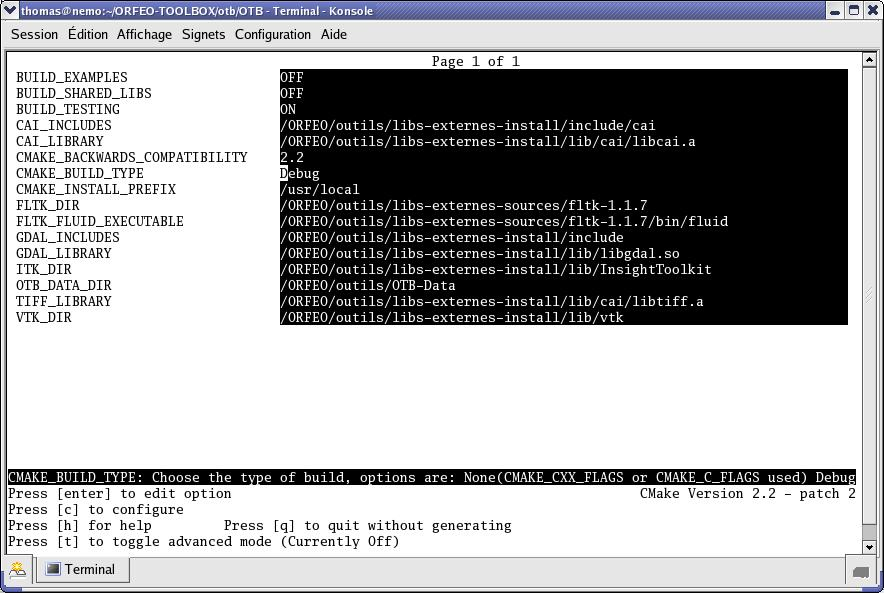
\includegraphics[width=0.8\textwidth]{ccmakeScreenShot.eps}
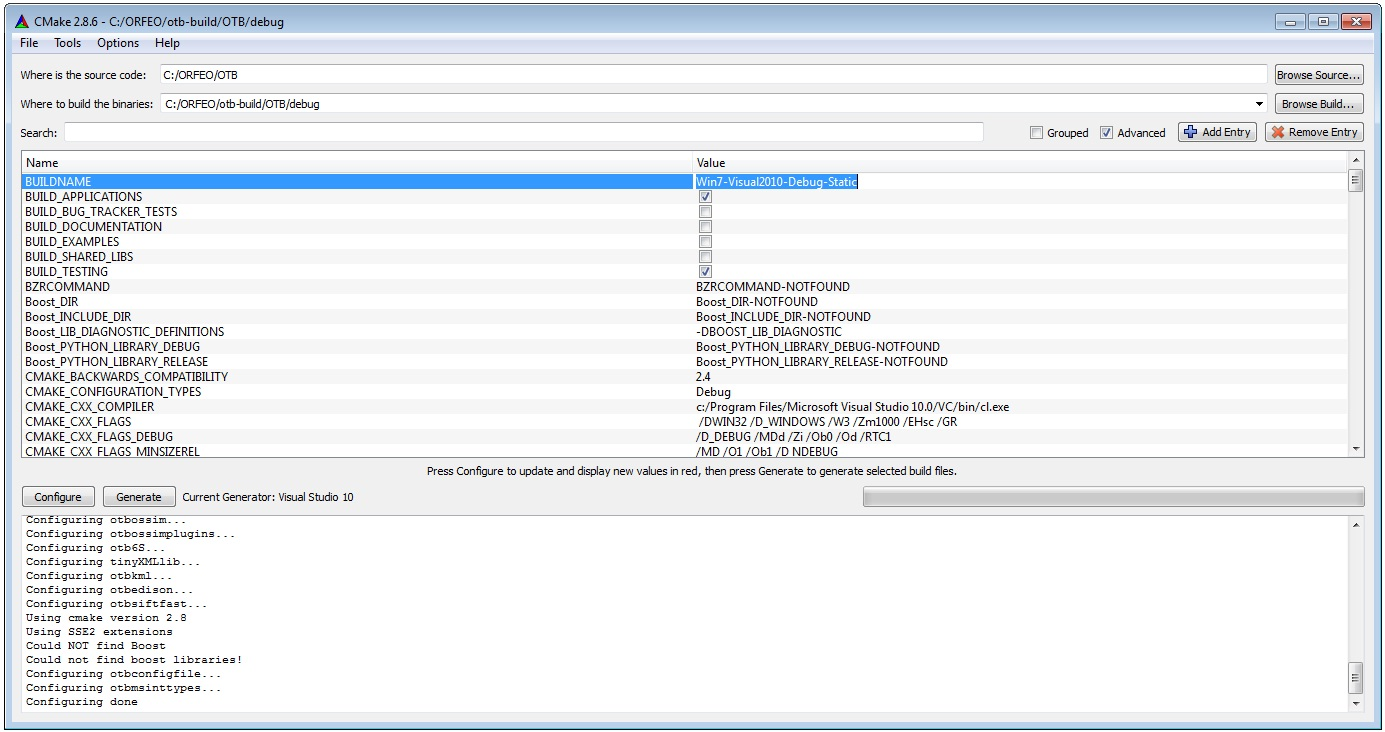
\includegraphics[width=0.8\textwidth]{CMakeSetupScreenShot.eps}
\itkcaption[Cmake user interface]{CMake interface. Top) \texttt{ccmake}, the UNIX
version based on \texttt{curses}. Bottom) \texttt{CMakeSetup}, the MS-Windows
version based on MFC.}
\label{fig:CMakeGUI}
\end{figure}

For more information on CMake, check :
\begin{center}
\url{http://www.cmake.org}
\end{center}

\index{Dependencies}
OTB depends on a number of external libraries.
Some are mandatory, meaning that OTB cannot be compiled without them, while others are optional and can be activated or
not during the build process.
See table \ref{tab:otb-dependencies} for the full list of dependencies.
\begin{center}
\begin{tiny}
\begin{table}[!htbp]
\begin{tabular}{|p{0.15\textwidth}|p{0.45\textwidth}|p{0.1\textwidth}|p{0.1\textwidth}|}
\hline
\textbf{Library} & \textbf{Web site} & \textbf{Mandatory} & \textbf{Minimum version} \\
\hline
\textbf{ITK} & \url{http://www.itk.org} & yes & 4.6.0 \\
\hline
\textbf{GDAL} & \url{http://www.gdal.org} & yes & 1.10 \\
\hline
\textbf{OSSIM} & \url{http://www.ossim.org} & yes & 1.8.20-3 \\
\hline
\textbf{Curl} & \url{http://www.curl.haxx.se} & no  & - \\
\hline
\textbf{FFTW} & \url{http://www.fftw.org} & no  & - \\
\hline
\textbf{libgeotiff} & \url{http://trac.osgeo.org/geotiff/} & yes & - \\
\hline
\textbf{OpenJPEG} & \url{http://code.google.com/p/openjpeg/} & no & - \\
\hline
\textbf{boost} & \url{http://www.boost.org} & yes & - \\
\hline
\textbf{openthreads} & \url{http://www.openscenegraph.org} & yes & - \\
\hline
\textbf{Mapnik} & \url{http://www.mapnik.org} & no  & - \\
\hline
\textbf{tinyXML} & \url{http://www.grinninglizard.com/tinyxml} & yes & - \\
\hline
\textbf{6S} & \url{http://6s.ltdri.org} & no & - \\
\hline
\textbf{SiftFast} & \url{http://libsift.sourceforge.net} & no  & - \\
\hline
\textbf{MuParser} & \url{http://www.muparser.sourceforge.net} & no  & - \\
\hline
\textbf{MuParserX} & \url{http://muparserx.beltoforion.de} & no  & 3.0.5 \\
\hline
\textbf{libSVM} & \url{http://www.csie.ntu.edu.tw/~cjlin/libsvm} & no  & 2.0 \\
\hline
\textbf{Qt} & \url{http://qt-project.org/} & no  & 4 \\
\hline
\textbf{OpenCV} & \url{http://opencv.org} & no  & 2 \\
\hline
\end{tabular}
\caption{External libraries used in OTB.}
\label{tab:otb-dependencies}
\end{table}
\end{tiny}
\end{center}

\section{Linux and Mac OS X}
\label{sec:compiling-linux}

\subsection{Setting up the build environment}

The first thing to do is to create a directory for working with OTB.
This guide will use \texttt{$\sim$/OTB} but you are free to choose something else.
In this directory, there will be three locations:
\begin{itemize}
\item \texttt{$\sim$/OTB/otb} for the source file obtained from the git repository
\item \texttt{$\sim$/OTB/build} for the intermediate build objects, CMake specific files, libraries and binaries.
\item \texttt{$\sim$/OTB/install}, the installation directory for OTB once it is built.
A system location (\texttt{/usr/local} for example) can also be used, but installing locally is more flexible and does
not require root access.
\end{itemize}
To setup this structure, the following commands can be used:
\begin{verbatim}
$ mkdir ~/OTB
$ cd ~/OTB
$ git clone https://git@git.orfeo-toolbox.org/git/otb.git
$ mkdir build
$ mkdir install
\end{verbatim}

The OTB project uses a git branching model where \texttt{develop} is the current development version.
It contains the latest patches and represents the work in progress towards the next release.
For more information on OTB and git, including how to decide which branch to want to compile, please see the
OTB wiki page at \url{http://wiki.orfeo-toolbox.org/index.php/Git}.

Checkout the relevant branch now:
\begin{verbatim}
$ cd ~/OTB/otb
$ git checkout develop
\end{verbatim}

Now you must decide which build method you will use.
There are two ways of compiling OTB from sources, depending on how you want to manage dependencies.
Both methods rely on CMake.
\begin{itemize}
\item SuperBuild (go to section~\ref{sec:installation-linux-superbuild}). All OTB dependencies are automatically downloaded and compiled.
This method is the easiest to use and provides a complete OTB with minimal effort.
\item Normal build (go to section~\ref{sec:installation-linux-normalbuild}). OTB dependencies must already be compiled and available on your system.
This method requires more work but provides more flexibility.
\end{itemize}
If you do not know which method to use and just want to compile OTB with all its modules, use SuperBuild.

\begin{center}
\begin{tiny}
\begin{table}[!htbp]
\begin{tabular}{p{0.35\textwidth}p{0.65\textwidth}}
\hline
\textbf{CMake variable} & \textbf{Value} \\
\hline
\texttt{CMAKE\_INSTALL\_PREFIX}         & Installation directory, target for \texttt{make install} \\
\texttt{BUILD\_EXAMPLES}                & Activate compilation of OTB examples \\
\texttt{BUILD\_TESTING}                 & Activate compilation of the tests \\
\texttt{OTB\_BUILD\_DEFAULT\_MODULES}   & Activate all usual modules, required to build the examples \\
\texttt{OTB\_USE\_\textit{XXX}}         & Activate module \textit{XXX} \\
\texttt{OTBGroup\_\textit{XXX}}         & Enable modules in the group \textit{XXX} \\
\texttt{OTB\_DATA\_ROOT}                & otb-data repository \\
\texttt{OTB\_WRAP\_PYTHON}              & Enable Python wrapper \\
\texttt{OTB\_WRAP\_JAVA}                & Enable Java wrapper \\

\hline
\multicolumn{2}{l}{\small \textbf{SuperBuild only}} \\ 
\texttt{DOWNLOAD\_LOCATION}             & Location to download dependencies \\
\texttt{USE\_SYSTEM\_\textit{XXX}}      & Use the system's \textit{XXX} library \\

\hline
\end{tabular}
\caption{Important CMake configuration variables in OTB}
\label{tab:installation-cmake-variables}
\end{table}
\end{tiny}
\end{center}

\subsection{SuperBuild: Build OTB and all dependencies}
\label{sec:installation-linux-superbuild}

The SuperBuild is a way of compiling dependencies to a project just before you build the project. Thanks to CMake and
its ExternalProject module, it is possible to download a source archive, configure and compile it when building
the main project. This feature has been used in other CMake-based projects (ITK, Slicer, ParaView,...).
In OTB, the SuperBuild is implemented with no impact on the library sources : the sources for SuperBuild are located in
the 'OTB/SuperBuild' subdirectory. It is made of CMake scripts and source patches that allow to compile all the
dependencies necessary for OTB. Once all the dependencies are compiled and installed, the OTB library is built using
those dependencies.

OTB's compilation is customized by specifying configuration variables.
The most important configuration variables are shown in table~\ref{tab:installation-cmake-variables}.
The simplest way to provide configuration variables is via the command line \texttt{-D} option:
\begin{verbatim}
$ cd ~/OTB/build
$ cmake -D CMAKE_INSTALL_PREFIX=~/OTB/install ../otb/SuperBuild
\end{verbatim}
A pre-load script can also be used with the \texttt{-C} options (see
\url{https://cmake.org/cmake/help/v3.4/manual/cmake.1.html#options}).
Another option is to set variables manually with \texttt{cmake-gui} or \texttt{ccmake}.

Please note that the \texttt{CMAKE\_INSTALL\_PREFIX} variable is important
because the SuperBuild will install some targets during the compilation step.
Therefore this directory will be used even if you don't use make install target.
In fact there is no make install target for the SuperBuild.

By default, SuperBuild will not use any of libraries installed on system. All \texttt{USE\_SYSTEM\_\textit{XXX}} are
are set to FALSE. This is our recommended way of using SuperBuild. You are however free to use a system library
if you want!. You must be very much aware of dependencies of those libraries you use from system. For example,
if libjpeg is not used from superbuild using \texttt{USE\_SYSTEM\_JPEG=TRUE} then you should not use zlib from superbuild
because zlib is a dependency of libjpeg. Here SuperBuild will not automagically set \texttt{USE\_SYSTEM\_ZLIB=FALSE}.
You must do it yourself. The example of libjpeg - zlib dependency chain is so simple.
Imagine the same case for GDAL which depends on zlib, libjpeg, libtiff(with big tiff support), geotiff,
sqlite, curl, geos, libkml, openjpeg. This is one of the reasons we recommend to use SuperBuild exclusively or not.

All dependencies are configured and built in a way that help us to get an efficient build OTB.
So we enable geotiff (with proj4 support), openjpeg, geos in GDAL build.

It is also important to note that SuperBuild is tested daily on all three platforms that makes us clear that
there is no issue with new changes in OTB and its dependencies. It simply works!

(see table~\ref{tab:installation-cmake-variables}).

SuperBuild downloads dependencies into the \texttt{DOWNLOAD\_LOCATION} directory, which will be
\texttt{$\sim$/OTB/build/Downloads} in our example.
Dependencies can be downloaded manually into this directory before the compilation step.
This can be usefull if you wish to bypass a proxy, intend to compile OTB without an internet conection, or other network
constraint. You can find an archive with sources of all our dependencies on the Orfeo ToolBox website (pick the 'SuperBuild-archives' corresponding to the OTB version you want to build) :
\begin{center}
\url{https://www.orfeo-toolbox.org/packages}
\end{center}

You are now ready to compile OTB!
Simply use the make command (other targets can be generated with CMake's \texttt{-G} option):
\begin{verbatim}
$ cd ~/OTB/build
$ make
\end{verbatim}

Applications will be located in the \texttt{bin/} directory, for example:
\begin{verbatim}
./OTB/build/bin/otbcli_ExtractROI
\end{verbatim}
will launch the command line version of the \textbf{ExtractROI} application,
while:
\begin{verbatim}
./OTB/build/bin/otbgui_ExtractROI
\end{verbatim}
will launch the graphical version.

We recommend adding OTB build directory to your PATH for easy access:
\begin{verbatim}
export PATH=$PATH:~/OTB/build/OTB/build/bin
\end{verbatim}

Monteverdi is also compiled by the SuperBuild (as long as you activate it with
ENABLE\_MONTEVERDI). To use OTB applications from within Monteverdi you will need
to define the OTB\_APPLICATION\_PATH environment variable.
\begin{verbatim}
export OTB_APPLICATION_PATH=~/OTB/build/OTB/build/lib/otb/applications
monteverdi
\end{verbatim}

A wiki page detailing the status of SuperBuild on various platforms is also available here:
\url{http://wiki.orfeo-toolbox.org/index.php/SuperBuild}.

\subsection{Normal build: Build only OTB}
\label{sec:installation-linux-normalbuild}

Once all OTB dependencies are availables on your system, use CMake to generate a Makefile:
\begin{verbatim}
$ cd ~/OTB/build
$ cmake -C configuration.cmake ../otb
\end{verbatim}
The script \texttt{configuration.cmake} needs to contain dependencies location if CMake cannot find them automatically.
This can be done with the \texttt{\textit{XXX}\_DIR} variables containing the directories which contain the
FindXXX.cmake scripts, or with the \texttt{\textit{XXX}\_INCLUDEDIR} and \texttt{\textit{XXX}\_LIBRARY} variables.

Additionally, decide which module you wish to enable, together with tests and examples.
Refer to table~\ref{tab:installation-cmake-variables} for the list of CMake variables.

Since OTB is modularized, it is possible to only build some modules instead of the whole set. 
To deactivate a module (and the ones that depend on it) switch off the CMake variable OTB\_BUILD\_DEFAULT\_MODULES,
configure, and then switch off each \texttt{Module\_module\_name} variable.
To provide an overview on how things work, the option \texttt{COMPONENTS} of the CMake command find\_package is used in
order to only load the requested modules.
This module-specific list prevent CMake from performing a blind search; it is also a convienent way to monitor the
dependencies of each module.
\begin{verbatim}
find_package(OTB COMPONENTS OTBCommon OTBTransform [...])
\end{verbatim} 

Some of the OTB capabilities are considered as optional, and you can deactivate the related modules thanks to a set of
CMake variables starting with \texttt{OTB\_USE\_\textit{XXX}}.
Table~\ref{tab:optional} shows which modules are associated to these variables. It is very important to notice that
these variable override the variable OTB\_BUILD\_DEFAULT\_MODULES.

You are now ready to compile OTB!
Simply use the make command (other targets can be generated with CMake's \texttt{-G} option):
\begin{verbatim}
$ make
\end{verbatim}

The installation target will copy the binaries and libraries to the installation location:
\begin{verbatim}
$ make install
\end{verbatim}

\begin{center}
\begin{tiny}
\begin{table}[!htbp]
\begin{tabular}{|l|l|p{0.52\textwidth}|}
\hline
\textbf{CMake variable} & \textbf{3rd party module} & \textbf{Modules depending on it} \\
\hline
\textbf{OTB\_USE\_LIBKML} & OTBlibkml & OTBKMZWriter OTBIOKML OTBAppKMZ \\
\hline
\textbf{OTB\_USE\_QT4} & OTBQt4 & OTBQtWidget \\
\hline
\textbf{OTB\_USE\_OPENCV} & OTBOpenCV & \\
\hline
\textbf{OTB\_USE\_MUPARSERX} & OTBMuParserX & OTBMathParserX OTBAppMathParserX \\
\hline
\textbf{OTB\_USE\_OPENJPEG} & OTBOpenJPEG & OTBIOJPEG2000 \\
\hline
\textbf{OTB\_USE\_CURL} & OTBCurl & \\
\hline
\textbf{OTB\_USE\_MUPARSER} & OTBMuParser & OTBMathParser OTBDempsterShafer OTBAppClassification OTBAppMathParser OTBAppStereo OTBAppProjection OTBAppSegmentation OTBAppClassification OTBRoadExtraction OTBRCC8 OTBCCOBIA OTBAppSegmentation OTBMeanShift OTBAppSegmentation OTBMeanShift OTBAppSegmentation \\
\hline
\textbf{OTB\_USE\_LIBSVM} & OTBLibSVM & OTBSVMLearning \\
\hline
\textbf{OTB\_USE\_MAPNIK} & OTBMapnik & OTBVectorDataRendering \\
\hline
\textbf{OTB\_USE\_6S} & OTB6S & OTBOpticalCalibration OTBAppOpticalCalibration OTBSimulation \\
\hline
\textbf{OTB\_USE\_SIFTFAST} & OTBSiftFast & \\
\hline
\end{tabular}
\caption{Third parties and related modules.}
\label{tab:optional}
\end{table}
\end{tiny}
\end{center}

\section{Windows}
\label{sec:compiling-windows}

Everything that is needed for OTB development on Windows, including compiling from source, is covered in details on the OTB wiki at:
\begin{center}
\url{http://wiki.orfeo-toolbox.org/index.php/OTB_development_on_Windows}
\end{center}

\section{Known issues}
\label{sec:knownissues}

\begin{itemize}
\item  openjpeg/ITK 
\end{itemize}

It is important to know that the OpenJpeg library doesn't support name mangling since version 2.0. 
As a consequence, if other libraries linked by your project already contain OpenJpeg, there may be a symbol conflict at run-time. 
For instance, this was observed with OTB build on a recent ITK version (ver. 4). 
The ITK library already had a version of OpenJpeg in libitkopenjpeg-*.so, which contained the OpenJpeg symbols un-wrapped.
These symbols were also loaded by the GDAL driver but only the first ones were used, which caused a crash. 

Hopefully, thanks to the modular architecture of ITK, the library libitkopenjpeg-*.so is not imported anymore inside OTB.
However the OpenJPEG headers may be present in ITK include directory. As the current architecture doesn't allow to tune 
include order between modules, the OpenJPEG header from ITK can be included before your own OpenJPEG install. There are
two ways to avoid this situation :
\begin{itemize}
\item Use an ITK without GDCM nor ITKReview (only these modules depend on OpenJPEG)
\item Hide the header openjpeg.h in the ITK include directory.
\end{itemize}

More information can be found here : \url{http://wiki.orfeo-toolbox.org/index.php/JPEG2000_with_GDAL_OpenJpeg_plugin}

\begin{itemize}
\item  libkml / Ubuntu 12.04 
\end{itemize}

Another issue is related to the official package of libkml under Ubuntu 12.4.
Until this problem is addressed, users of this plateform should disable the option OTB\_USE\_KML, so that OTB won't be built with this third-party.


\chapter{System Overview}
\label{chapter:SystemOverview}

The purpose of this chapter is to provide you with an overview of the
\emph{ORFEO Toolbox} system. We recommend that you read this chapter to
gain an appreciation for the breadth and area of application of
OTB. In this chapter, we will make reference either to \emph{OTB
  features} or \emph{ITK features} without distinction. Bear in mind
that OTB uses ITK as its core element, so all the fundamental elements
of OTB come from ITK. OTB extends the functionalities of ITK for the
remote sensing image processing comunity. We benefit from the Open
Source development approach chosen for ITK, which allows us to provide
an impressive set of functionalities with much lesser effort than it
would have been the case in a closed source universe!

\section{System Organization}
\label{sec:SystemOrganization}

The ORFEO Toolbox consists of several subsystems. A brief
description of these subsystems follows. Later sections in this chapter---and
in some cases additional chapters---cover these concepts in more detail. (Note:
in the previous chapter two other modules---\code{OTB-Documents} and
\code{OTB-Applications} were briefly described.)

\begin{description}
	\item[Essential System Concepts.] Like any software system, OTB is
        built around some core design concepts. OTB uses those of
        ITK. Some of the more important
        concepts include generic programming, smart pointers for memory
        management, object factories for adaptable object instantiation,
        event management using the command/observer design paradigm, and
        multithreading support.

	\item[Numerics] OTB, as ITK uses VXL's VNL numerics libraries. These are
        easy-to-use C++ wrappers around the Netlib Fortran numerical 
        analysis routines (\url{http://www.netlib.org}).

	\item[Data Representation and Access.]  Two principal classes
        are used to represent data: the \doxygen{otb}{Image} and
        \doxygen{itk}{Mesh} classes.  In addition, various types of
        iterators and containers are used in ITK to hold and traverse
        the data. Other important but less popular classes are also
        used to represent data such as histograms.

	\item[ITK's Data Processing Pipeline.]  The data representation
	classes (known as \emph{data objects}) are operated on by
	\emph{filters} that in turn may be organized into data flow
	\emph{pipelines}. These pipelines maintain state and therefore
	execute only when necessary.  They also support
	multi-threading, and are streaming capable (i.e., can operate
	on pieces of data to minimize the memory footprint).

        \item[IO Framework.] Associated with the data processing
        pipeline are \emph{sources}, filters that initiate the
        pipeline, and \emph{mappers}, filters that terminate the
        pipeline.  The standard examples of sources and mappers are
        \emph{readers} and \emph{writers} respectively.  Readers
        input data (typically from a file), and writers output data
        from the pipeline. \emph{Viewers} are another example of mappers.

	\item[Spatial Objects.] Geometric shapes are represented in
        OTB using the ITK spatial object hierarchy.  These classes are
        intended to support modeling of anatomical structures in
        ITK. OTB uses them in order to model cartographic elements. Using a
        common basic interface, the spatial objects are capable of
        representing regions of space in a variety of different
        ways. For example: mesh structures, image masks, and implicit
        equations may be used as the underlying representation scheme.
        Spatial objects are a natural data structure for communicating
        the results of segmentation methods and for introducing
        geometrical priors in both segmentation and registration
        methods.

	\item[ITK's Registration Framework.] A flexible framework for
        registration supports four different types of registration:
        image registration, multiresolution registration, PDE-based
        registration, and FEM (finite element method) registration.

	\item[FEM Framework.] ITK includes a subsystem for solving general
        FEM problems, in particular non-rigid registration. The FEM package
        includes mesh definition (nodes and elements), loads, and boundary
        conditions.

	\item[Level Set Framework.] The level set framework is a set of
        classes for creating filters to solve partial differential equations
        on images using an iterative, finite difference update scheme. The
        level set framework consists of finite difference solvers including a
        sparse level set solver, a generic level set segmentation filter, and
        several specific subclasses including threshold, Canny, and Laplacian
        based methods.

	\item[Wrapping.] ITK uses a unique, powerful system for
	producing interfaces (i.e., ``wrappers'') to interpreted
	languages such as Tcl and Python. The GCC\_XML tool is used to
	produce an XML description of arbitrarily complex C++ code;
	CSWIG is then used to transform the XML description into
	wrappers using the \href{http://www.swig.org/}{SWIG}
	package. OTB does not use this system at present.

%% 	\item[Auxiliary / Utilities] Several auxiliary subsystems are 
%%         available to supplement other classes in the system. For example,
%%         calculators are classes that perform specialized operations in
%%         support of filters (e.g., MeanCalculator computes the mean of a
%%         sample). Other utilities include GDAL format file
%%         support, png, zlib, FLTK / Qt image viewers, and interfaces to the
%%         Visualization Toolkit (VTK) system.
        
\end{description}


\section{Essential System Concepts}
\label{sec:EssentialSystemConcepts}

This section describes some of the core concepts and implementation features
found in ITK and therefore also in OTB.

\subsection{Generic Programming}
\label{sec:GenericProgramming}

\index{generic programming}
\index{template}

Generic programming is a method of organizing libraries consisting of
generic---or reusable---software components \cite{Musser1996}. The idea is to
make software that is capable of ``plugging together'' in an efficient,
adaptable manner. The essential ideas of generic programming are
\emph{containers} to hold data, \emph{iterators} to access the data, and 
\emph{generic algorithms} that use containers and iterators to create 
efficient, fundamental algorithms such as sorting. Generic programming is
implemented in C++ with the \emph{template} programming mechanism and the 
use of the STL Standard Template Library \cite{Austern1999}.

C++ templating is a programming technique allowing users to write software in
terms of one or more unknown types \code{T}. To create executable code, the
user of the software must specify all types \code{T} (known as \emph{template
instantiation}) and successfully process the code with the compiler. The
\code{T} may be a native type such as
\code{float} or \code{int}, or \code{T} may be a user-defined type (e.g.,
\code{class}). At compile-time, the compiler makes sure that the templated 
types are compatible with the instantiated code and that the types are
supported by the necessary methods and operators.

ITK uses the techniques of generic programming in its implementation. The
advantage of this approach is that an almost unlimited variety of data types
are supported simply by defining the appropriate template types. For example,
in OTB it is possible to create images consisting of almost any type of
pixel. In addition, the type resolution is performed at compile-time, so the
compiler can optimize the code to deliver maximal performance. The
disadvantage of generic programming is that many compilers still do not
support these advanced concepts and cannot compile OTB. And even if they do,
they may produce completely undecipherable error messages due to even the
simplest syntax errors. If you are not familiar with templated code and
generic programming, we recommend the two books cited above.

\subsection{Include Files and Class Definitions}
\label{sec:IncludeFiles}

In ITK and OTB classes are defined by a maximum of two files: a header \code{.h} file
and an implementation file---\code{.cxx} if a non-templated class, and a
\code{.txx} if a templated class.
The header files contain class declarations
and formatted comments that are used by the Doxygen documentation
system to automatically produce HTML manual pages.

In addition to class headers, there are a few other important header files.
\begin{description}
        \item[\code{itkMacro.h}] is found in the
        \code{Utilities/ITK/Code/Common} directory
        and defines standard system-wide macros (such as \code{Set/Get},
        constants, and other parameters).

        \item[\code{itkNumericTraits.h}] is found in the \code{Utilities/ITK/Code/Common}
        directory and defines numeric characteristics for native types such
        as its maximum and minimum possible values.

        \item[\code{itkWin32Header.h}] is found in the \code{Utilities/ITK/Code/Common}
        and is used to define operating system parameters to control
        the compilation process.
\end{description}

\subsection{Object Factories}
\label{sec:ObjectFactories}

\index{object factory}
\index{factory}

Most classes in OTB are instantiated through an \emph{object factory}
mechanism. That is, rather than using the standard C++ class constructor and
destructor, instances of an OTB class are created with the static class
\code{New()} method. In fact, the constructor and destructor are
\code{protected:} so it is generally not possible to construct an OTB
instance on the heap. (Note: this behavior pertains to classes that are
derived from \doxygen{itk}{LightObject}. In some cases the need for speed or
reduced memory footprint dictates that a class not be derived from
LightObject and in this case instances may be created on the heap. An
example of such a class is \doxygen{itk}{EventObject}.)

The object factory enables users to control run-time instantiation of classes
by registering one or more factories with \doxygen{itk}{ObjectFactoryBase}. These
registered factories support the method \code{CreateInstance(classname)}
which takes as input the name of a class to create. The factory can choose to
create the class based on a number of factors including the computer system
configuration and environment variables. For example, in a particular
application an OTB user may wish to deploy their own class implemented using
specialized image processing hardware (i.e., to realize a performance
gain). By using the object factory mechanism, it is possible at run-time to
replace the creation of a particular OTB filter with such a custom class. (Of
course, the class must provide the exact same API as the one it is
replacing.) To do this, the user compiles her class (using the same compiler,
build options, etc.) and inserts the object code into a shared library or
DLL. The library is then placed in a directory referred to by the
\code{OTB\_AUTOLOAD\_PATH} environment variable. On instantiation, the object
factory will locate the library, determine that it can create a class of a
particular name with the factory, and use the factory to create the
instance. (Note: if the \code{CreateInstance()} method cannot find a factory
that can create the named class, then the instantiation of the class falls
back to the usual constructor.)

In practice object factories are used mainly (and generally transparently) by
the OTB input/output (IO) classes. For most users the greatest impact is on
the use of the \code{New()} method to create a class. Generally the
\code{New()} method is declared and implemented via the macro
\code{itkNewMacro()} found in \code{Utilities/ITK/Common/itkMacro.h}.


\subsection{Smart Pointers and Memory Management}
\label{sec:SmartPointers}

\index{smart pointer}

By their nature object-oriented systems represent and operate on data through
a variety of object types, or classes. When a particular class is
instantiated to produce an instance of that class, memory allocation occurs
so that the instance can store data attribute values and method pointers
(i.e., the vtable). This object may then be referenced by other classes or
data structures during normal operation of the program. Typically during
program execution all references to the instance may disappear at which point
the instance must be deleted to recover memory resources. Knowing when to
delete an instance, however, is difficult. Deleting the instance too soon
results in program crashes; deleting it too late and memory leaks (or
excessive memory consumption) will occur. This process of allocating and
releasing memory is known as memory management.

In ITK, memory management is implemented through reference counting. This
compares to another popular approach---garbage collection---used
\index{garbage collection} by many
systems including Java. In reference counting, a count of the number of
references to each instance is kept. When the reference goes to zero, the
object destroys itself. In garbage collection, a background process sweeps
the system identifying instances no longer referenced in the system and
deletes them. The problem with garbage collection is that the actual point in
time at which memory is deleted is variable. This is unacceptable when an
object size may be gigantic (think of a large 3D volume gigabytes in
size). Reference counting deletes memory immediately (once all references to
an object disappear).

Reference counting is implemented through a \code{Register()}/\code{Delete()}
member function interface.  All instances of an OTB object have a
\code{Register()} method invoked on them by any other object that references
an them. The \code{Register()} method increments the instances' reference
count. When the reference to the instance disappears, a \code{Delete()}
method is invoked on the instance that decrements the reference count---this
is equivalent to an \code{UnRegister()} method. When the reference count
returns to zero, the instance is destroyed.

This protocol is greatly simplified by using a helper class called a
\doxygen{itk}{SmartPointer}. The smart pointer acts like a regular pointer
(e.g. supports operators \code{->} and \code{*}) but automagically performs a
\code{Register()} when referring to an instance, and an \code{UnRegister()}
when it no longer points to the instance.  Unlike most other instances in
OTB, SmartPointers can be allocated on the program stack, and are
automatically deleted when the scope that the SmartPointer was created
is closed. As a result, you should \emph{rarely if ever call Register() or
Delete()} in OTB. For example:

\small
\begin{verbatim}
  MyRegistrationFunction()
    { <----- Start of scope

    // here an interpolator is created and associated to the
    // SmartPointer "interp".
    InterpolatorType::Pointer interp = InterpolatorType::New();

    } <------ End of scope
\end{verbatim}
\normalsize

In this example, reference counted objects are created (with the \code{New()}
method) with a reference count of one. Assignment to the SmartPointer
\code{interp} does not change the reference count. At the end of scope,
\code{interp} is destroyed, the reference count of the actual interpolator
object (referred to by \code{interp}) is decremented, and if it reaches zero,
then the interpolator is also destroyed.

Note that in ITK SmartPointers are always used to refer to instances of
classes derived from \doxygen{itk}{LightObject}. Method invocations and function
calls often return ``real'' pointers to instances, but they are immediately
assigned to a SmartPointer. Raw pointers are used for non-LightObject classes when
the need for speed and/or memory demands a smaller, faster class.


\subsection{Error Handling and Exceptions}
\label{sec:ErrorHandling}

\index{exceptions}
\index{error handling}

In general, OTB uses exception handling to manage errors during program
execution. Exception handling is a standard part of the C++ language and
generally takes the form as illustrated below:
\small
\begin{verbatim}
  try
    {
    //...try executing some code here...
    }
  catch ( itk::ExceptionObject exp )
    {
    //...if an exception is thrown catch it here
    }
\end{verbatim}
\normalsize

where a particular class may throw an exceptions as demonstrated below (this
code snippet is taken from \doxygen{itk}{ByteSwapper}:
\small
\begin{verbatim}
  switch ( sizeof(T) )
    {
    //non-error cases go here followed by error case  
    default:  
      ByteSwapperError e(__FILE__, __LINE__);
      e.SetLocation("SwapBE");
      e.SetDescription("Cannot swap number of bytes requested");
      throw e;
    }
\end{verbatim}
\normalsize

Note that \doxygen{itk}{ByteSwapperError} is a subclass of
\doxygen{itk}{ExceptionObject}. (In fact in OTB all exceptions should be derived
from \code{itk::ExceptionObject}.) In this example a special constructor and C++
preprocessor variables \code{\_\_FILE\_\_} and \code{\_\_LINE\_\_} are used to instantiate
the exception object and provide additional information to the user. You can
choose to catch a particular exception and hence a specific OTB error, or you
can trap \emph{any} OTB exception by catching ExceptionObject.


\subsection{Event Handling}
\label{sec:EventHandling}

\index{event handling}
\index{Command/Observer design pattern}
\index{itk::Command}
\index{ProgressEvent()}
\index{InvokeEvent()}

Event handling in OTB is implemented using the Subject/Observer design
pattern \cite{Gamma1995} (sometimes referred to as the Command/Observer
design pattern). In this approach, objects indicate that they are watching
for a particular event---invoked by a particular instance--by registering
with the instance that they are watching.  For example, filters in OTB
periodically invoke the \doxygen{itk}{ProgressEvent}. Objects that have registered
their interest in this event are notified when the event occurs. The
notification occurs via an invocation of a command (i.e., function callback,
method invocation, etc.) that is specified during the registration
process. (Note that events in OTB are subclasses of EventObject; look
in \code{itkEventObject.h} to determine which events are available.)

To recap via example: various objects in OTB will invoke specific events
as they execute (from ProcessObject):
\small
\begin{verbatim}
  this->InvokeEvent( ProgressEvent() );
\end{verbatim}
\normalsize

To watch for such an event, registration is required that associates a
command (e.g., callback function) with the event:
\code{Object::AddObserver()} method:
\small
\begin{verbatim}
  unsigned long progressTag = 
    filter->AddObserver(ProgressEvent(), itk::Command*);
\end{verbatim}
\normalsize

When the event occurs, all registered observers are notified via invocation
of the associated \code{Command::Execute()} method. Note that several
subclasses of Command are available supporting const and
non-const member functions as well as C-style functions. (Look in
\code{Common/Command.h} to find pre-defined subclasses of
Command. If nothing suitable is found, derivation is another
possibility.)

\subsection{Multi-Threading}
\label{sec:MultiThreading}

Multithreading is handled in OTB through ITK's high-level design
abstraction. This approach provides portable multithreading and hides the
complexity of differing thread implementations on the many systems supported
by OTB. For example, the class \doxygen{itk}{MultiThreader} provides support for
multithreaded execution using \code{sproc()} on an SGI, or
\code{pthread\_create} on any platform supporting POSIX threads. 

Multithreading is typically employed by an algorithm during its execution
phase. MultiThreader can be used to execute a single method on
multiple threads, or to specify a method per thread. For example, in the 
class \doxygen{itk}{ImageSource} (a superclass for most image processing filters)
the \code{GenerateData()} method uses the following methods:

\small
\begin{verbatim}
  multiThreader->SetNumberOfThreads(int);
  multiThreader->SetSingleMethod(ThreadFunctionType, void* data);
  multiThreader->SingleMethodExecute();
\end{verbatim}
\normalsize

In this example each thread invokes the same method. The multithreaded filter
takes care to divide the image into different regions that do not overlap for
write operations.

The general philosophy in ITK regarding thread safety is that accessing
different instances of a class (and its methods) is a thread-safe operation.
Invoking methods on the same instance in different threads is to be avoided.


\section{Numerics}
\label{sec:Numerics}

\index{VNL}
\index{numerics}

OTB; as ITK, uses the VNL numerics library to provide resources for numerical
programming combining the ease of use of packages like Mathematica and Matlab
with the speed of C and the elegance of C++. It provides a C++ interface to
the high-quality Fortran routines made available in the public domain by
numerical analysis researchers. ITK extends the functionality of VNL
by including interface classes between VNL and ITK proper.

The VNL numerics library includes classes for
\begin{description}
        \item[Matrices and vectors.] Standard matrix and vector support
        and operations on these types.

        \item[Specialized matrix and vector classes.] Several special matrix
        and vector class with special numerical properties are
        available. Class \code{vnl\_diagonal\_matrix} provides a fast and
        convenient diagonal matrix, while fixed size matrices and vectors
        allow "fast-as-C" computations (see \code{vnl\_matrix\_fixed<T,n,m>} 
        and example subclasses \code{vnl\_double\_3x3} and 
        \code{vnl\_double\_3}).

        \item[Matrix decompositions.] Classes \code{vnl\_svd<T>}, 
        \code{vnl\_symmetric\_eigensystem<T>}, and 
        \code{vnl\_generalized\_eigensystem}. 

        \item[Real polynomials.] Class \code{vnl\_real\_polynomial} stores 
        the coefficients of a real polynomial, and provides methods of 
        evaluation of the polynomial at any x, while class 
        \code{vnl\_rpoly\_roots} provides a root finder. 

        \item[Optimization.] Classes \code{vnl\_levenberg\_marquardt},
        \code{vnl\_amoeba}, \code{vnl\_conjugate\_gradient}, 
        \code{vnl\_lbfgs} allow optimization of user-supplied
        functions either with or without user-supplied derivatives.

        \item[Standardized functions and constants.] Class \code{vnl\_math}
        defines constants (pi, e, eps...) and simple functions (sqr, abs,
        rnd...). Class \code{numeric\_limits} is from the ISO standard
        document, and provides a way to access basic limits of a
        type. For example \code{numeric\_limits<short>::max()} returns the maximum
        value of a short.
\end{description}

Most VNL routines are implemented as wrappers around the high-quality Fortran
routines that have been developed by the numerical analysis community over
the last forty years and placed in the public domain. The central repository
for these programs is the "netlib" server \url{http://www.netlib.org/}. The
National Institute of Standards and Technology (NIST) provides an excellent
search interface to this repository in its \emph{Guide to Available Mathematical
Software (GAMS)} at \url{http://gams.nist.gov}, both as a decision tree and a
text search.

ITK also provides additional numerics functionality. A suite of optimizers, that
use VNL under the hood and integrate with the registration framework
are available. A large collection of statistics functions---not available from
VNL---are also provided in the \code{Insight/Numerics/Statistics}
directory. In addition, a complete finite element (FEM) package is available,
primarily to support the deformable registration in ITK.


\section{Data Representation}
\label{sec:DataRepresentationAndAccess}
%	mesh, image, iterators, various containers

\index{data object} 

There are two principal types of data represented in OTB: images and
meshes. This functionality is implemented in the classes 
Image and Mesh, both of which are subclasses of
\doxygen{itk}{DataObject}. In OTB, data objects are classes that are meant to
be passed around the system and may participate in data flow pipelines (see
Section~\ref{sec:DataProcessingPipeline} on
page~\pageref{sec:DataProcessingPipeline} for more information).


\index{otb::Image}

\doxygen{otb}{Image} represents an \emph{n}-dimensional, regular sampling of
data. The sampling direction is parallel to each of the coordinate axes, and
the origin of the sampling, inter-pixel spacing, and the number of samples in
each direction (i.e., image dimension) can be specified. The sample, or
pixel, type in OTB is arbitrary---a template parameter \code{TPixel}
specifies the type upon template instantiation. (The dimensionality of the
image must also be specified when the image class is instantiated.) The key
is that the pixel type must support certain operations (for example, addition
or difference) if the code is to compile in all cases (for example, to be
processed by a particular filter that uses these operations). In practice the
OTB user will use a C++ simple type (e.g., \code{int}, \code{float}) or a pre-defined pixel
type and will rarely create a new type of pixel class.

One of the important ITK concepts regarding images is that rectangular,
continuous pieces of the image are known as \emph{regions}. Regions are used
to specify which part of an image to process, for example in multithreading,
or which part to hold in memory. In ITK there are three common types of
regions:
\begin{enumerate}
\item \code{LargestPossibleRegion}---the image in its entirety.
\item \code{BufferedRegion}---the portion of the image retained in memory.
\item \code{RequestedRegion}---the portion of the region requested by a 
filter or other class when operating on the image.
\end{enumerate}

The \doxygen{otb}{Image} class extends the functionalities of the
\doxygen{itk}{Image} in order to take into account particular remote
sensing features as geographical projections, etc.

\index{itk::Mesh} 

The Mesh class represents an \emph{n}-dimensional, unstructured grid. The
topology of the mesh is represented by a set of \emph{cells} defined by a 
type and
connectivity list; the connectivity list in turn refers to points.  The
geometry of the mesh is defined by the \emph{n}-dimensional points in
combination with associated cell interpolation functions. \code{Mesh} is
designed as an adaptive representational structure that changes depending on
the operations performed on it. At a minimum, points and cells are required
in order to represent a mesh; but it is possible to add additional topological
information.  For example, links from the points to the cells that use each
point can be added; this provides implicit neighborhood information assuming
the implied topology is the desired one. It is also possible to
specify boundary cells explicitly, to indicate different connectivity
from the implied neighborhood relationships, or to store information
on the boundaries of cells. 

The mesh is defined in terms of three template parameters: 1) a pixel type
associated with the points, cells, and cell boundaries; 2) the dimension of
the points (which in turn limits the maximum dimension of the cells); and 3)
a ``mesh traits'' template parameter that specifies the types of the
containers and identifiers used to access the points, cells, and/or
boundaries. By using the mesh traits carefully, it is possible to create
meshes better suited for editing, or those better suited for ``read-only''
operations, allowing a trade-off between representation flexibility, memory,
and speed.

Mesh is a subclass of \doxygen{itk}{PointSet}. The PointSet
class can be used to represent point clouds or randomly distributed
landmarks, etc. The PointSet class has no associated topology.


\section{Data Processing Pipeline}
\label{sec:DataProcessingPipeline}

\index{data processing pipeline}

\index{process object} 
\index{source}
\index{reader} 
\index{filter} 
\index{mapper} 

While data objects (e.g., images and meshes) are used to represent data,
\emph{process objects} are classes that operate on data objects and may
produce new data objects. Process objects are classed as
\emph{sources}, \emph{filter objects}, or \emph{mappers}.  Sources (such as
readers) produce data, filter objects take in data and process it to produce
new data, and mappers accept data for output either to a file or
some other system.  Sometimes the term \emph{filter} is used broadly
to refer to all three types.

\index{streaming}

The data processing pipeline ties together data objects (e.g., images and
meshes) and process objects. The pipeline supports an automatic updating
mechanism that causes a filter to execute if and only if its input 
or its internal state changes. Further, the data pipeline supports
\emph{streaming}, the ability to automatically break data into smaller
pieces, process the pieces one by one, and reassemble the processed data into
a final result.

Typically data objects and process objects are connected together using the
\code{SetInput()} and \code{GetOutput()} methods as follows:

\small
\begin{verbatim}
  typedef otb::Image<float,2> FloatImage2DType;

  itk::RandomImageSource<FloatImage2DType>::Pointer random;
  random = itk::RandomImageSource<FloatImage2DType>::New();
  random->SetMin(0.0);
  random->SetMax(1.0);

  itk::ShrinkImageFilter<FloatImage2DType,FloatImage2DType>::Pointer shrink;
  shrink = itk::ShrinkImageFilter<FloatImage2DType,FloatImage2DType>::New();
  shrink->SetInput(random->GetOutput());
  shrink->SetShrinkFactors(2);

  otb::ImageFileWriter::Pointer<FloatImage2DType> writer;
  writer = otb::ImageFileWriter::Pointer<FloatImage2DType>::New();
  writer->SetInput (shrink->GetOutput());
  writer->SetFileName( ``test.raw'' );
  writer->Update();
\end{verbatim}
\normalsize 

In this example the source object \doxygen{itk}{RandomImageSource} is connected
to the \doxygen{itk}{ShrinkImageFilter}, and the shrink filter is connected to
the mapper \doxygen{otb}{ImageFileWriter}. When the \code{Update()} method is
invoked on the writer, the data processing pipeline causes each of these
filters in order, culminating in writing the final data to a file on disk.

%\section{Registration Framework}
%\label{sec:RegistrationFramework}
%
%blah blah
%
%\section{FEM Framework}
%\label{sec:FEMFramework}
%
%blah blah
%
\section{Spatial Objects}
\label{sec:SpatialObjectsOverview}
\index{spatial object}
%
The ITK spatial object framework supports the philosophy that the task of
image segmentation and registration is actually the task of object
processing. The image is but one medium for representing objects of interest,
and much processing and data analysis can and should occur at the object
level and not based on the medium used to represent the object.

ITK spatial objects provide a common interface for accessing the physical
location and geometric properties of and the relationship between objects in
a scene that is independent of the form used to represent those objects. That
is, the internal representation maintained by a spatial object may be a list
of points internal to an object, the surface mesh of the object, a continuous
or parametric representation of the object's internal points or surfaces, and
so forth.

The capabilities provided by the spatial objects framework supports their use
in object segmentation, registration, surface/volume rendering, and other
display and analysis functions. The spatial object framework extends the
concept of a ``scene graph'' \index{scene graph} that is common to computer rendering packages so
as to support these new functions. With the spatial objects framework you
can:
\begin{enumerate}

        \item Specify a spatial object's parent and children objects.  In
        this way, a city may contain roads and those roads can be
        organized in a tree structure.

        \item Query if a physical point is inside an object or
        (optionally) any of its children.

        \item Request the value and derivatives, at a physical point,
        of an associated intensity function, as specified
        by an object or (optionally) its children.

        \item Specify the coordinate transformation that maps a parent
        object's coordinate system into a child object's coordinate system.

        \item Compute the bounding box of a spatial object and (optionally)
        its children.

        \item Query the resolution at which the object was originally
        computed.  For example, you can query the resolution (i.e., pixel
        spacing) of the image used to generate a particular instance of a
        \doxygen{itk}{LineSpatialObject}.
\end{enumerate}

Currently implemented types of spatial objects include: Blob, Ellipse,
Group, Image, Line, Surface, and Tube.  The \doxygen{itk}{Scene}
object is used to hold a list of spatial objects that may in turn have
children.  Each spatial object can be assigned a color property.  Each
spatial object type has its own capabilities. For example,
\doxygen{itk}{TubeSpatialObject}s indicate to what point on their parent
tube they connect.

There are a limited number of spatial objects and their methods in ITK, but
their number is growing and their potential is huge. Using the nominal
spatial object capabilities, methods such as mutual
information registration, can be applied to objects regardless of their
internal representation. By having a common API, the same method can be used
to register a parametric representation of a building with an image or
to register two different segmentations of a particular object in
object-based change detection.

%blah blah
%
%\section{Level Set Framework}
%\label{sec:LevelSetFramework}
%
%blah blah
%
%% \section{Wrapping}
%% \label{sec:Wrapping}

%% \index{wrapping}
%% \index{Tcl}
%% \index{Python}

%% While the core of OTB is implemented in C++, Tcl and Python bindings can be
%% automatically generated and OTB programs can be created using these
%% programming languages. This capability is under active development and is for
%% the advanced user only. However, this brief description will give you an idea
%% of what is possible and where to look if you are interested in this facility.

%% The wrapping process in OTB is quite complex due to the use of generic
%% programming (i.e., extensive use of C++ templates). Systems like VTK that use
%% their own wrapping facility are non-templated and customized to the coding
%% methodology found in the system. Even systems like SWIG that are designed
%% for general wrapper generation have difficulty with OTB code because general
%% C++ is difficult to parse. As a result, the OTB wrapper generator uses a
%% combination of tools to produce language bindings.
%% \begin{enumerate}
%%   \item gccxml is a modified version of the GNU compiler gcc that
%%     produces an XML description of an input C++ program.
%%   \item  CABLE processes XML information from gccxml and produces
%%     additional input to the next tool (i.e., CSWIG indicating what is
%%     to be wrapped).
%%   \item CSWIG is a modified version of SWIG that has SWIG's usual
%%     parser replaced with an XML parser (XML produced from CABLE and
%%     gccxml.) CSWIG produces the appropriate language bindings
%%     (either Tcl or Python). (Note: since SWIG is capable of producing
%%     language bindings for eleven different interpreted languages including
%%     Java, and Perl, it is expected that support for some of these languages
%%     will be added in the future.)
%% \end{enumerate}

%% To learn more about the wrapping process, please read the file found in
%% \code{Wrapping/CSwig/README}. Also note that there are some simple test
%% scripts found in \code{Wrapping/CSwig/Tests}. Additional tests and examples
%% are found in the {Testing/Code/*/} directories.

%% The result of the wrapping process is a set of shared libraries/dll's that
%% can be used by the interpreted languages. There is almost a direct
%% translation from C++, with the differences being the particular syntactical
%% requirements of each language. For example, in the directory
%% \code{Testing/Code/Algorithms}, the test
%% \code{itkCurvatureFlowTestTcl2.tcl} has a code fragment that appears as
%% follows: 
%% \small
%% \begin{verbatim}
%%   set reader [itkImageFileReaderF2_New]
%%     $reader SetFileName "${OTB_TEST_INPUT}/cthead1.png"

%%   set cf [itkCurvatureFlowImageFilterF2F2_New]
%%     $cf SetInput [$reader GetOutput]
%%     $cf SetTimeStep 0.25
%%     $cf SetNumberOfIterations 10
%% \end{verbatim}
%% \normalsize
%% The same code in C++ would appear as follows:

%% \small
%% \begin{verbatim}
%%   otb::ImageFileReader<ImageType>::Pointer reader = 
%%               otb::ImageFileReader<ImageType>::New();
%%   reader->SetFileName("cthead1.png");

%%   itk::CurvatureFlowImageFilter<ImageType,ImageType>::Pointer cf =
%%       itk::CurvatureFlowImageFilter<ImageType,ImageType>::New();
%%     cf->SetInput(reader->GetOutput());
%%     cf->SetTimeStep(0.25);
%%     cf->SetNumberOfIterations(10);
%% \end{verbatim}
%% \normalsize

%% This example demonstrates an important difference between C++ and a wrapped
%% language such as Tcl.  Templated classes must be instantiated prior to
%% wrapping. That is, the template parameters must be specified as part of the
%% wrapping process. In the example above, the
%% \code{CurvatureFlowImageFilterF2F2} indicates that this filter has been
%% instantiated using an input and output image type of two-dimensional float
%% values (e.g., \code{F2}). Typically just a few common types are selected for
%% the wrapping process to avoid an explosion of types and hence, library
%% size. To add a new type requires rerunning the wrapping process to produce
%% new libraries.

%% The advantage of interpreted languages is that they do not require the
%% lengthy compile/link cycle of a compiled language like C++. Moreover, they
%% typically come with a suite of packages that provide useful
%% functionality. For example, the Tk package (i.e., Tcl/Tk and Python/Tk)
%% provides tools for creating sophisticated user interfaces. In the future it
%% is likely that more applications and tests will be implemented in the various
%% interpreted languages supported by OTB.


%
%blah blah
%
%\section{Auxiliary \& Utilities}
%\label{sec:Auxiliary}
%\label{sec:Utilities}
%
%calculators and classes supporting the data processing pipeline;
%utilities such as GUI interface tools

\fi


\part{User's guide}

\ifitkFullVersion
\chapter{Data Representation}
\label{sec:DataRepresentation}


This chapter introduces the basic classes responsible
for representing data in OTB. The most common classes are the
\doxygen{otb::Image}, the \doxygen{itk::Mesh} and the \doxygen{itk::PointSet}.

\section{Image}
\label{sec:ImageSection}

The \doxygen{otb::Image} class follows the spirit of
\href{http://www.boost.org/more/generic_programming.html}{Generic
Programming}, where types are separated from the algorithmic behavior
of the class.  OTB supports images with any pixel type and any spatial
dimension.

\subsection{Creating an Image}\label{sec:CreatingAnImageSection}

\textbf{FIXME : update with otb::Image}
\input{Image1.tex}

In practice it is rare to allocate and initialize an image directly.
Images are typically read from a source, such a file or data acquisition
hardware. The following example illustrates how an image can be read from
a file.




\subsection{Reading an Image from a File}
\label{sec:ReadingImageFromFile}

\input{Image2.tex}





\subsection{Accessing Pixel Data}
\label{sec:AccessingImagePixelData}

\input{Image3.tex}




\subsection{Defining Origin and Spacing}
\label{sec:DefiningImageOriginAndSpacing}

\input{Image4.tex}

\subsection{Defining Other Image Attributes}
\label{sec:DefiningOtherImageAttributes}
%% Geographic projections, etc?

\subsection{RGB Images}

The term RGB (Red, Green, Blue) stands for a color representation commonly used
in digital imaging. RGB is a representation of the human physiological
capability to analyze visual light using three spectral-selective
sensors~\cite{Malacara2002,Wyszecki2000}. The human retina possess different
types of light sensitive cells. Three of them, known as \emph{cones}, are
sensitive to color~\cite{Gray2003} and their regions of sensitivity loosely
match regions of the spectrum that will be perceived as red, green and blue
respectively. The \emph{rods} on the other hand provide no color discrimination
and favor high resolution and high sensitivity\footnote{The human eye is
capable of perceiving a single isolated photon.}.  A fifth type of receptors,
the \emph{ganglion cells}, also known as circadian\footnote{The term
\emph{Circadian} refers to the cycle of day and night, that is, events that are
repeated with 24 hours intervals.} receptors are sensitive to the lighting
conditions that differentiate day from night.  These receptors evolved as a
mechanism for synchronizing the physiology with the time of the day. Cellular
controls for circadian rythms are present in every cell of an organism and are
known to be exquisitively precise~\cite{Lodish2000}.

The RGB space has been constructed as a representation of a physiological
response to light by the three types of \emph{cones} in the human eye. RGB is
not a Vector space. For example, negative numbers are not appropriate in a
color space because they will be the equivalent of ``negative stimulation'' on
the human eye.  In the context of colorimetry, negative color values are used
as an artificial construct for color comparison in the sense that

\begin{equation}
\label{eqn:ColorSubtraction}
         ColorA = ColorB - ColorC
\end{equation}

just as a way of saying that we can produce $ColorB$ by combining $ColorA$ and
$ColorC$.  However, we must be aware that (at least in emitted light) it is not
possible to \emph{substract light}. So when we mention
Equation~\ref{eqn:ColorSubtraction} we actually mean

\begin{equation}
\label{eqn:ColorAddition}
         ColorB = ColorA + ColorC
\end{equation}

On the other hand, when dealing with printed color and with paint, as opposed
to emitted light like in computer screens, the physical behavior of color
allows for subtraction. This is because strictly speaking the objects that we
see as red are those that absorb all light frequencies except those in the red
section of the spectrum~\cite{Wyszecki2000}.

The concept of addition and subtraction of colors has to be carefully
interpreted. In fact, RGB has a different definition regarding whether we are
talking about the channels associated to the three color sensors of the human
eye, or to the three phosphors found in most computer monitors or to the color
inks that are used for printing reproduction.  Color spaces are usually non
linear and do not even from a Group. For example, not all visible colors can be
represented in RGB space~\cite{Wyszecki2000}.

ITK introduces the \doxygen{RGBPixel} type as a support for representing the
values of an RGB color space. As such, the RGBPixel class embodies a different
concept from the one of an \doxygen{Vector} in space. For this reason, the
RGBPixel lack many of the operators that may be naively expected from it. In
particular, there are no defined operations for subtraction or addition.

When you anticipate to perform the operation of ``Mean'' on a RGB type you are
assuming that in the color space provides the action of finding a color in the
middle of two colors, can be found by using a linear operation between their
numerical representation. This is unfortunately not the case in  color spaces
due to the fact that they are based on a human physiological
response~\cite{Malacara2002}.

If you decide to interpret RGB images as simply three independent channels then
you should rather use the \doxygen{Vector} type as pixel type. In this way, you
will have access to the set of operations that are defined in Vector spaces.
The current implementation of the RGBPixel in ITK presumes that RGB color
images are intended to be used in applications where a formal interpretation of
color is desired, therefore only the operations that are valid in a color space
are available in the RGBPixel class.

The following example illustrates how RGB images can be represented in ITK.

\label{sec:DefiningRGBImages}
%\input{RGBImage.tex}


\subsection{Vector Images}
%\label{sec:DefiningVectorImages}

%\input{VectorImage.tex}


\subsection{Importing Image Data from a Buffer}
\label{sec:ImportingImageDataFromABuffer}
%\input{Image5.tex}



\section{PointSet}
\label{PointSetSection}

\subsection{Creating a PointSet}
\label{sec:CreatingAPointSet}

%\input{PointSet1.tex}



\subsection{Getting Access to Points}
\label{sec:GettingAccessToPointsInThePointSet}

%\input{PointSet2.tex}



\subsection{Getting Access to Data in Points}
\label{sec:GettingAccessToDataInThePointSet}

%\input{PointSet3.tex}



\subsection{RGB as Pixel Type}
\label{sec:PointSetWithRGBAsPixelType}

%\input{RGBPointSet.tex}




\subsection{Vectors as Pixel Type}
\label{sec:PointSetWithVectorsAsPixelType}

%\input{PointSetWithVectors.tex}



\subsection{Normals as Pixel Type}
\label{sec:PointSetWithCovariantVectorsAsPixelType}

%\input{PointSetWithCovariantVectors.tex}




\section{Mesh}\label{MeshSection}

\subsection{Creating a Mesh}
\label{sec:CreatingAMesh}

%\input{Mesh1.tex}


\subsection{Inserting Cells}
\label{sec:InsertingCellsInMesh}

%\input{Mesh2.tex}


\subsection{Managing Data in Cells}
\label{sec:ManagingCellDataInMesh}

%\input{Mesh3.tex}


\subsection{Customizing the Mesh}
\label{sec:CustomizingTheMesh}

%\input{MeshTraits.tex}


\subsection{Topology and the K-Complex}
\label{sec:MeshKComplex}

%\input{MeshKComplex.tex}


\subsection{Representing a PolyLine}
\label{sec:MeshPolyLine}

%\input{MeshPolyLine.tex}


\subsection{Simplifying Mesh Creation}
\label{sec:AutomaticMesh}

%\input{AutomaticMesh.tex}


\subsection{Iterating Through Cells}
\label{sec:MeshCellsIteration}

%\input{MeshCellsIteration.tex}


\subsection{Visiting Cells}
\label{sec:MeshCellVisitor}

%\input{MeshCellVisitor.tex}


\subsection{More on Visiting Cells}
\label{sec:MeshCellVisitorMultipleType}

%\input{MeshCellVisitor2.tex}




\section{Path}\label{PathSection}

\subsection{Creating a PolyLineParametricPath}
\label{sec:CreatingAPolyLineParametricPath}

%\input{PolyLineParametricPath1.tex}

\section{Containers}\label{ContainersSection}
\label{sec:TreeContainer}
%\input{TreeContainer.tex}




2;rgb:0000/0000/0000\chapter{Reading and Writing Images}
\label{sec:IO}

This chapter describes the toolkit architecture supporting reading and
writing of images to files. OTB does not enforce any particular file
format, instead, it provides a structure inherited from ITK,
supporting a variety of formats that can be easily extended by the
user as new formats become available.

We begin the chapter with some simple examples of file I/O.

\section{Basic Example}
\label{sec:ImagReadWrite}
\input{ImageReadWrite.tex}

To better understand the IO architecture, please refer to Figures
\ref{fig:ImageIOCollaborationDiagram},
\ref{fig:ImageIOFactoriesUseCases}, and
\ref{fig:ImageIOFactoriesClassDiagram}.

\begin{figure}
\center
\includegraphics[width=\textwidth]{ImageIOCollaborationDiagram.eps}
\itkcaption[Collaboration diagram of the ImageIO classes]{Collaboration diagram
of the ImageIO classes.} \label{fig:ImageIOCollaborationDiagram}
\end{figure}

\begin{figure}
\center
\includegraphics[width=\textwidth]{ImageIOFactoriesUseCases.eps}
\itkcaption[Use cases of ImageIO factories] {Use cases of ImageIO factories.}
\label{fig:ImageIOFactoriesUseCases}
\end{figure}

\begin{figure}
\center
\includegraphics[width=\textwidth]{ImageIOFactoriesClassDiagram.eps}
\itkcaption[Class diagram of ImageIO factories] {Class diagram of the ImageIO
factories.}
\label{fig:ImageIOFactoriesClassDiagram}
\end{figure}


The following section describes the internals of the IO architecture provided
in the toolbox.

\section{Pluggable Factories}
\label{sec:ImageIOPluggableFactories}

The principle behind the input/output mechanism used in ITK and
therefore OTB is known as
\emph{pluggable-factories} \cite{Gamma1995}. This concept is illustrated in
the UML diagram in Figure~\ref{fig:ImageIOCollaborationDiagram}. From the
user's point of view the objects responsible for reading and writing files
are the \doxygen{otb}{ImageFileReader} and \doxygen{otb}{ImageFileWriter}
classes. These two classes, however, are not aware of the details involved in
reading or writing particular file formats like PNG or GeoTIFF.  What they do
is to dispatch the user's requests to a set of specific classes that are
aware of the details of image file formats. These classes are the
\doxygen{itk}{ImageIO} classes. The ITK delegation mechanism enables users to
extend the number of supported file formats by just adding new classes to the
ImageIO hierarchy.

Each instance of ImageFileReader and ImageFileWriter has
a pointer to an ImageIO object. If this pointer is empty, it will
be impossible to read or write an image and the image file reader/writer must
determine which ImageIO class to use to perform IO operations.
This is done basically by passing the filename to a centralized class, the
\doxygen{itk}{ImageIOFactory} and asking it to identify any subclass of
ImageIO capable of reading or writing the user-specified file. This
is illustrated by the use cases on the right side of
Figure~\ref{fig:ImageIOFactoriesUseCases}. The ImageIOFactory acts here as a
dispatcher that help to locate the actual IO factory classes corresponding to
each file format.

Each class derived from ImageIO must provide an associated factory
class capable of producing an instance of the ImageIO class. For
example, for PNG files, there is a \doxygen{itk}{PNGImageIO} object that knows how
to read this image files and there is a \doxygen{itk}{PNGImageIOFactory} class
capable of constructing a PNGImageIO object and returning a pointer
to it.  Each time a new file format is added (i.e., a new ImageIO
subclass is created), a factory must be implemented as a derived class of the
ObjectFactoryBase class as illustrated in
Figure~\ref{fig:ImageIOFactoriesClassDiagram}.

For example, in order to read PNG files, a PNGImageIOFactory is
created and registered with the central ImageIOFactory
singleton\footnote{\emph{Singleton} means that there is only one instance of
this class in a particular application} class as illustrated in the left side
of Figure~\ref{fig:ImageIOFactoriesUseCases}. When the ImageFileReader asks
the ImageIOFactory for an ImageIO capable of reading the
file identified with \emph{filename} the ImageIOFactory will iterate over the
list of registered factories and will ask each one of them is they know how
to read the file. The factory that responds affirmatively will be used to
create the specific ImageIO instance that will be returned to the
ImageFileReader and used to perform the read operations.

With respect to the ITK formats, OTB adds most of the remote sensing
image formats. In order to do so, the Geospatial Data Abstraction Library, GDAL
      \url{http://www.gdal.org/}, is encapsultated in a ImageIO
      factory. GDAL is a translator library for raster
      geospatial data formats that is released under an X/MIT style
      Open Source license. As a library, it presents a single abstract
      data model to the calling application for all supported formats,
      which include CEOS, GeoTIFF, ENVI, and much more. See
      \url{http://www.gdal.org/formats_list.html} for
      the full format list.

      Since GDAL is itself a multi-format library, the GDAL IO
factory is able to choose the appropriate resource for reading and
writing images.

In most cases the mechanism is transparent to the user who only interacts
with the ImageFileReader and ImageFileWriter. It is
possible, however, to explicitly select the type of ImageIO object
to use.  Please see the ITK Software for more details about this.

%\section{Using ImageIO Classes Explicitly}
%\label{sec:ImageReadExportVTK}
%\input{ImageReadExportVTK.tex}

\section{IO Streaming}
\index{Streaming}
\label{sec:IOStreaming}
\subsection{Implicit Streaming}
\label{sec:ImplicitIOStreaming}
\input{StreamingImageReadWrite}

\subsection{Explicit Streaming}
\label{sec:ExplicitIOStreaming}
\input{ExplicitStreamingExample}


\section{Reading and Writing RGB Images}
\index{Image!RGB}
\label{sec:RGBImagReadWrite}
\input{RGBImageReadWrite.tex}

\section{Reading, Casting and Writing Images}
\label{sec:ImagReadCastWrite}
\input{ImageReadCastWrite.tex}

\section{Extracting Regions}
\label{sec:ImagReadRegionOfInterestWrite}
\input{ImageReadRegionOfInterestWrite.tex}

%\section{Extracting Slices}
%\label{sec:ImagReadExtractWrite}
%\input{ImageReadExtractWrite.tex}


\section{Reading and Writing Vector Images}
\index{Image!Multispectral}
\label{sec:VectorImagReadWrite}

Images whose pixel type is a Vector, a CovariantVector, an Array, or a Complex
are quite common in image processing. One of the uses of these tye of
images is the processing of SLC SAR images, which are complex.


%\subsection{The Minimal Example}
%\label{VectorImageReadWrite}
%\input{VectorImageReadWrite.tex}

%\subsection{Producing and Writing Covariant Images}
%\label{CovariantVectorImageWrite}
%\input{CovariantVectorImageWrite.tex}

%\subsection{Reading Covariant Images}
%\label{CovariantVectorImageRead}
%Let's now take the image that we just created and read it into another program.
%\input{CovariantVectorImageRead.tex}


\subsection{Reading and Writing Complex Images}
\label{sec:ComplexImagReadWrite}
\input{ComplexImageReadWrite.tex}

\section{Reading and Writing Multiband Images}
\label{sec:MultibandImagReadWrite}
\input{MultibandImageReadWrite.tex}

\subsection{Extracting ROIs}
\label{sec:ExtractROI}
\input{ExtractROI.tex}


%\section{Extracting Components from Vector Images}
%\label{sec:VectorImageExtractComponent}
%\input{CovariantVectorImageExtractComponent.tex}

\section{Reading Image Series}
\label{sec:ReadingImageSeries}
\input{ImageSeriesIOExample}


\section{Extended filename for reader and writer}
\label{sec:ExtendedFilename}

\subsection{Purpose}

There are multiple ways to define geo-referencing information. For instance,
 one can use a geographic transform, a cartographic projection, or a sensor 
model with RPC coefficients. A single image may contain several of these 
elements, such as in the "ortho-ready" products : this is a type of product 
still in sensor geometry (the sensor model is supplied with the image) 
but it also contains an approximative geographic transform that can be used 
to have a quick estimate of the image localisation. For instance, your product
may contain a ".TIF" file for the image, along with a ".RPB" file that contains
the sensor model coefficients and an ".IMD" file that contains a cartographic 
projection. 

This case leads to the following question : which geo-referencing element
should be used when opening this image in an OTB reader. In fact, it depends on
the users need. For an orthorectification application, the sensor model must be
used. In order to specify which information should be skipped, a syntax of 
extended filenames has been developed for both reader and writer. 


\subsection{Syntax}

The reader and writer extended file name support is based on the same syntax,
only the options are different.  To benefit from the extended file name
mechanism, the following syntax is to be used:

\begin{verbatim}
Path/Image.ext?&key1=<value1>&key2=<value2>
\end{verbatim}

IMPORTANT: Note that you'll probably need to "quote" the filename.

\subsection{Reader options}

\textbf{Available Options:}

\begin{itemize}

\item \begin{verbatim}&geom=<path/filename.geom>\end{verbatim}

  \begin{itemize}
  \item Contains the file name of a valid geom file
  \item Use the content of the specified geom file instead of image-embedded
    geometric information
  \item empty by default, use the image-embedded information if available
  \end{itemize}  
\item \begin{verbatim}&sdataidx=<(int)idx>\end{verbatim}
  \begin{itemize}
  \item Select the sub-dataset to read
  \item 0 by default
  \end{itemize}
\item \begin{verbatim}&resol=<(int)resolution factor>\end{verbatim}
  \begin{itemize}
  \item Select the JPEG2000 sub-resolution image to read
  \item 0 by default
  \end{itemize}
\item \begin{verbatim}&band=r1,r2,...,rn\end{verbatim}
\begin{itemize}
    \item Select a subset of bands from the input image
    \item The syntax is inspired by Python indexing syntax with
      band=r1,r2,r3,...,rn  where each ri is a band range that can be :
      \begin{itemize}
      \item a single index (1-based) :
        \begin{itemize}
          \item $'2'$ means 2nd band
          \item $'-1'$ means last band
          \end{itemize}
        \item or a range of bands :
          \begin{itemize}
            \item $'3:'$ means 3rd band until the last one
            \item $':-2'$ means the first bands until the second to last
            \item $'2:4'$ means bands 2,3 and 4
          \end{itemize}
      \end{itemize}
    \item empty by default (all bands are read from the input image) 
\end{itemize}
\item \begin{verbatim}&skipcarto=<(bool)true>\end{verbatim}
  \begin{itemize}
  \item Skip the cartographic information
  \item Clears the projectionref, set the origin to $[0,0]$ and the spacing to $[1/max(1,resolution factor),1/max(1,resolution factor)]$
  \item Keeps the keyword list
  \item false by default 
  \end{itemize}
\item \begin{verbatim}&skipgeom=<(bool)true>\end{verbatim}
  \begin{itemize}
  \item Skip geometric information
  \item Clears the keyword list
  \item Keeps the projectionref and the origin/spacing information
  \item false by default. 
  \end{itemize}
\item \begin{verbatim}&skiprpctag=<(bool)true>\end{verbatim}
  \begin{itemize}
  \item Skip the reading of internal RPC tags (see \ref{sec:TypesofSensorModels} for details)
  \item false by default. 
  \end{itemize}
\end{itemize}

\subsection{Writer options}

\textbf{Available Options:}

\begin{itemize}

\item \begin{verbatim}&writegeom=<(bool)false>\end{verbatim}
  \begin{itemize}
  \item To activate writing of external geom file
  \item true by default
  \end{itemize}  
\item \begin{verbatim}&writerpctags=<(bool)true>\end{verbatim}
  \begin{itemize}
  \item To activate writing of RPC tags in TIFF files
  \item false by default
  \end{itemize}  
\item \begin{verbatim}&gdal:co:<GDALKEY>=<VALUE>\end{verbatim}
  \begin{itemize}
  \item To specify a gdal creation option
  \item For gdal creation option information, see dedicated gdal documentation
  \item None by default 
  \end{itemize}
\item \begin{verbatim}&streaming:type=<VALUE>\end{verbatim}
  \begin{itemize}
  \item Activates configuration of streaming through extended filenames
  \item Override any previous configuration of streaming
  \item Allows to configure the kind of streaming to perform
  \item Available values are:
    \begin{itemize}
    \item auto : tiled or stripped streaming mode chosen automatically depending on TileHint read from input files
    \item tiled : tiled streaming mode
    \item stripped : stripped streaming mode
    \item none : explicitly deactivate streaming 
    \end{itemize}
  \item Not set by default 
  \end{itemize}
\item \begin{verbatim}&streaming:sizemode=<VALUE>\end{verbatim}
  \begin{itemize}
  \item Allows to choose how the size of the streaming pieces is computed
  \item Available values are:
    \begin{itemize}
    \item auto  : size is estimated from the available memory setting by evaluating pipeline memory print
    \item height : size is set by setting height of strips or tiles
    \item nbsplits : size is computed from a given number of splits 
    \end{itemize}
  \item Default is auto 
  \end{itemize}
\item \begin{verbatim}&streaming:sizevalue=<VALUE>\end{verbatim}
\begin{itemize}
    \item Parameter for size of streaming pieces computation
    \item Value is :
      \begin{itemize}
        \item if sizemode=auto : available memory in Mb
        \item if sizemode=height : height of the strip or tile in pixels
        \item if sizemode=nbsplits : number of requested splits for streaming 
      \end{itemize}
    \item If not provided, the default value is set to 0 and result in different behaviour depending on sizemode (if set to height or nbsplits, streaming is deactivated, if set to auto, value is fetched from configuration or cmake configuration file) 
\end{itemize}

\item \begin{verbatim}&box=<startx>:<starty>:<sizex>:<sizey>\end{verbatim}
\begin{itemize}
    \item User defined parameters of output image region
    \item The region must be set with 4 unsigned integers (the separator used is
      the colon ':'). Values are:
      \begin{itemize}
        \item startx: first index on X (starting with 0)
        \item starty: first index on Y (starting with 0)
        \item sizex: size along X
        \item sizey: size along Y 
      \end{itemize}
    \item The definition of the region follows the same convention as itk::Region
    definition in C++. A region is defined by two classes: the itk::Index and
    itk::Size classes. The origin of the region within the image with which it
    is associated is defined by Index 
\end{itemize}

\end{itemize}

The available syntax for boolean options are:

\begin{itemize}
    \item ON, On, on, true, True, 1 are available for setting a 'true' boolean value
    \item OFF, Off, off, false, False, 0 are available for setting a 'false' boolean value
\end{itemize}
%% \section{Reading and Writing Image Series}

%% It is still quite common to store 3D medical images in sets of files each one
%% containing a single slice of a volume dataset. Those 2D files can be read as
%% individual 2D images, or can be grouped together in order to reconstruct a 3D
%% dataset. The same practice can be extended to higher dimensions, for example,
%% for managing 4D datasets by using sets of files each one containing a 3D image.
%% This practice is common in the domain of cardiac imaging, perfusion, functional
%% MRI and PET. This section illustrates the functionalities available in ITK for
%% dealing with reading and writing series of images.

%% \index{Series!Reading}
%% \index{Series!Writing}
%% \index{Image Series!Reading}
%% \index{Image Series!Writing}

%% \subsection{Reading Image Series}
%% \label{sec:ReadingImageSeries}
%% \input{ImageSeriesReadWrite.tex}

%% \subsection{Writing Image Series}
%% \label{sec:WritingImageSeries}
%% %\input{ImageReadImageSeriesWrite.tex}

%% \subsection{Reading and Writing Series of RGB Images}
%% \label{sec:ReadingWritingRGBImageSeries}
%% %\input{RGBImageSeriesReadWrite.tex}




\chapter{Basic Filtering}


This chapter introduces the most commonly used filters found in OTB.
Most of these filters are intended to process images. They will accept one or
more images as input and will produce one or more images as output. OTB is
based ITK's data pipeline architecture in which the output of one filter is
passed as input to another filter. (See Section
\ref{sec:DataProcessingPipeline} on page \pageref{sec:DataProcessingPipeline}
for more information.)


\section{Thresholding}
\ifitkFullVersion
\label{sec:ThresholdingFiltering}
\fi

The thresholding operation is used to change or identify pixel values based
on specifying one or more values (called the \emph{threshold} value). The
following sections describe how to perform thresholding operations using
OTB.

\subsection{Binary Thresholding}
\label{sec:BinaryThresholdingImageFilter}

\ifitkFullVersion
\input{BinaryThresholdImageFilter.tex}
\fi

\subsection{General Thresholding}
\label{sec:ThresholdingImageFilter}

\ifitkFullVersion
\input{ThresholdImageFilter.tex}
\fi

\subsection{Threshold to Point Set}
\label{sec:ThresholdImageToPointSetFilter}

\ifitkFullVersion
\input{ThresholdToPointSetExample.tex}
\fi


%% \section{Casting and Intensity Mapping}
%% \label{sec:CastingImageFilters}

%% The filters discussed in this section perform pixel-wise intensity mappings.
%% Casting is used to convert one pixel type to another, while intensity mappings
%% also take into account the different intensity ranges of the pixel types.

%% \subsection{Linear Mappings}
%% \label{sec:IntensityLinearMapping}

%% \ifitkFullVersion
%% %\input{CastingImageFilters.tex}
%% \fi

%% \subsection{Non Linear Mappings}
%% \label{sec:IntensityNonLinearMapping}

%% The following filter can be seen as a variant of the casting filters. Its main
%% difference is the use of a smooth and continuous transition function of
%% non-linear form.

%% \ifitkFullVersion
%% %\input{SigmoidImageFilter.tex}
%% \fi

\section{Mathematical operations on images}
OTB and ITK provide a lot of filters allowing to perform basic operations on image layers (thresholding, ratio, layers combinations...).
It allows to create a processing chain defining at each step operations and to combine them in the data pipeline.
But the library offers also the possibility to perform more generic complex mathematical operation on images in a single filter: the
\doxygen{otb}{BandMathImageFilter} and more recently the \doxygen{otb}{BandMathImageFilterX}.

\subsection{BandMath filter}
\label{sec:BandMathImageFilter}

\ifitkFullVersion
\input{BandMathFilterExample.tex}
\fi

\subsection{BandMathX filter}
\label{sec:BandMathImageFilterX}
A new version of the BandMath filter is now available; among the new functionalities, variables representing multi-band pixels were introduced, as well as variables representing neighborhoods of pixels. The class name is \doxygen{otb}{BandMathImageFilterX}.

\ifitkFullVersion
\input{BandMathXImageFilterExample.tex}
\fi

\section{Gradients}
\label{sec:GradientFiltering}

Computation of gradients is a fairly common operation in image processing. The
term ``gradient'' may refer in some contexts to the gradient vectors and in
others to the magnitude of the gradient vectors. ITK filters attempt to
reduce this ambiguity by including the \emph{magnitude} term when
appropriate. ITK provides filters for computing both the image of gradient
vectors and the image of magnitudes.

\subsection{Gradient Magnitude}
\label{sec:GradientMagnitudeImageFilter}

\ifitkFullVersion
\input{GradientMagnitudeImageFilter.tex}
\fi

\subsection{Gradient Magnitude With Smoothing}
\label{sec:GradientMagnitudeRecursiveGaussianImageFilter}

\ifitkFullVersion
\input{GradientMagnitudeRecursiveGaussianImageFilter.tex}
\fi


\subsection{Derivative Without Smoothing}
\label{sec:DerivativeImageFilter}

\ifitkFullVersion
\input{DerivativeImageFilter.tex}
\fi


\section{Second Order Derivatives}
\label{sec:SecondOrderDerivatives}


%% \subsection{Second Order Recursive Gaussian}
%% \label{sec:SecondDerivativeRecursiveGaussian}

%% \ifitkFullVersion
%% \input{SecondDerivativeRecursiveGaussianImageFilter.tex}
%% \fi


\subsection{Laplacian Filters}
\label{sec:LaplacianFilters}

%\subsubsection{Laplacian Filter Finite Difference}
\subsubsection{Laplacian Filter Recursive Gaussian}
\ifitkFullVersion
\input{LaplacianRecursiveGaussianImageFilter1.tex}
\input{LaplacianRecursiveGaussianImageFilter2.tex}
\fi




\section{Edge Detection}

\subsection{Canny Edge Detection}
\ifitkFullVersion
\input{CannyEdgeDetectionImageFilter.tex}
\fi

\subsection{Ratio of Means Detector}
\input{TouziEdgeDetectorExample}



\section{Neighborhood Filters}
\label{sec:NeighborhoodFilters}

The concept of locality is frequently encountered in image processing in the
form of filters that compute every output pixel using information from a small
region in the neighborhood of the input pixel.  The classical form of
these filters are the $3 \times 3$ filters in 2D images. Convolution masks
based on these neighborhoods can perform diverse tasks ranging from noise
reduction, to differential operations, to mathematical morphology.

The Insight toolkit implements an elegant approach to neighborhood-based image
filtering.  The input image is processed using a special iterator called the
\doxygen{itk}{NeighborhoodIterator}. This iterator is capable of moving over all the
pixels in an image and, for each position, it can address the pixels in a local
neighborhood. Operators are defined that apply an algorithmic operation in the
neighborhood of the input pixel to produce a value for the output pixel.  The
following section describes some of the more commonly used filters that take
advantage of this construction. (See Chapter
\ref{sec:ImageIteratorsChapter} on page
\pageref{sec:ImageIteratorsChapter} for more information about iterators.)

\subsection{Mean Filter}
\label{sec:MeanFilter}

\ifitkFullVersion
#Add a dependency of "CircleMeanOutput.png" on "Circle.png".
ADD_GENERATED_FIG_DEPS( "CircleMeanOutput.png" "Circle.png" )
# Cmake macro to invoke: /ORFEO/thomas/ORFEO-TOOLBOX/otb/OTB/Examples/Data/MeanImageFilter  /Circle.png /CircleMeanOutput.png 10 10
RUN_EXAMPLE( "MeanImageFilter" "CircleMeanOutput.png" "/ORFEO/thomas/ORFEO-TOOLBOX/otb/OTB/Examples/StartExamples/MeanImageFilter.cxx"  /Circle.png /CircleMeanOutput.png 10 10 )
CONVERT_IMG( "Circle.png" "Circle.eps" "" )
ADD_DEP_TEX_ON_EPS_FIGS( "/ORFEO/thomas/ORFEO-TOOLBOX/otb/OTB-Documents/SoftwareGuide/Art/Generated" "Circle.eps" )
CONVERT_IMG( "CircleMeanOutput.png" "CircleMeanOutput.eps" "" )
ADD_DEP_TEX_ON_EPS_FIGS( "/ORFEO/thomas/ORFEO-TOOLBOX/otb/OTB-Documents/SoftwareGuide/Art/Generated" "CircleMeanOutput.eps" )

\fi

\subsection{Median Filter}
\label{sec:MedianFilter}

\ifitkFullVersion
\input{MedianImageFilter.tex}
\fi


\subsection{Mathematical Morphology}
\label{sec:MathematicalMorphology}

Mathematical morphology has proved to be a powerful resource for image
processing and analysis \cite{Serra1982}. ITK implements mathematical
morphology filters using NeighborhoodIterators and
\doxygen{itk}{NeighborhoodOperator}s.  The toolkit contains two types of image
morphology algorithms, filters that operate on binary images and filters that
operate on grayscale images.

\subsubsection{Binary Filters}
\label{sec:MathematicalMorphologyBinaryFilters}

\ifitkFullVersion
\input{MathematicalMorphologyBinaryFilters.tex}
\fi


\subsubsection{Grayscale Filters}
\label{sec:MathematicalMorphologyGrayscaleFilters}

\ifitkFullVersion
\input{MathematicalMorphologyGrayscaleFilters.tex}
\fi


%% \subsection{Voting Filters}
%% \label{sec:VotingFilters}

%% Voting filters are quite a generic family of filters. In fact, both the Dilate
%% and Erode filters from Mathematical Morphology are very particular cases of the
%% broader family of voting filters. In a voting filter, the outcome of a pixel is
%% decided by counting the number of pixels in its neighborhood and applying a
%% rule to the result of that counting.For example, the typical implementation of
%% Erosion in terms of a voting filter will be to say that a foreground pixel will
%% become background if the numbers of background neighbors is greater or equal
%% than 1. In this context, you could imagine variations of Erosion in which the
%% count could be changed to require at least 3 foreground.

%% \subsubsection{Binary Median Filter}

%% One of the particular cases of Voting filters is the BinaryMedianImageFilter.
%% This filter is equivalent to applying a Median filter over a binary image. The
%% fact of having a binary image as input makes possible to optimize the execution
%% of the filter since there is no real need for sorting the pixels according to
%% their frequency in the neighborhood.

%% \ifitkFullVersion
%% %\input{BinaryMedianImageFilter.tex}
%% \fi

%% The typical effect of median filtration on a noisy digital image is a dramatic reduction in impulse noise spikes. The filter also tends to preserve brightness differences across signal steps, resulting in reduced blurring of regional boundaries. The filter also tends to preserve the positions of boundaries in an image.

%% Figure \ref{fig:BinaryMedianImageFilterOutputMultipleIterations} below shows the effect of running the median filter with a 3x3 classical window size
%% 1, 10 and 50 times. There is a tradeoff in noise reduction and the sharpness of the image when the window size is increased\begin{figure}
%%   \center
%%   \includegraphics[width=0.44\textwidth]{BinaryMedianImageFilterOutput1.eps}
%%   \includegraphics[width=0.44\textwidth]{BinaryMedianImageFilterOutput10.eps}
%%   \includegraphics[width=0.44\textwidth]{BinaryMedianImageFilterOutput50.eps}
%%   \itkcaption[Effect of many iterations on the BinaryMedian filter.]{Effect of 1, 10 and 50 iterations of the
%%   BinaryMedianImageFilter using a 3x3 window.}
%%   \label{fig:BinaryMedianImageFilterOutputMultipleIterations}
%% \end{figure}.


%% \subsubsection{Hole Filling Filter}

%% Another variation of Voting filters is the Hole Filling filter. This filter
%% converts background pixels into foreground only when the number of foreground
%% pixels is a majority of the neighbors. By selecting the size of the majority,
%% this filter can be tuned to fill-in holes of different size. To be more
%% precise, the effect of the filter is actually related to the curvature of the
%% edge in which the pixel is located.

%% \ifitkFullVersion
%% %\input{VotingBinaryHoleFillingImageFilter.tex}
%% \fi


%% \subsubsection{Iterative Hole Filling Filter}

%% The Hole Filling filter can be used in an iterative way, by applying it
%% repeatedly until no pixel changes. In this context, the filter can be seen as a
%% binary variation of a Level Set filter.

%% \ifitkFullVersion
%% %\input{VotingBinaryIterativeHoleFillingImageFilter.tex}
%% \fi

\section{Smoothing Filters}
\label{sec:SmoothingFilters}

Real image data has a level of uncertainty that is manifested in the
variability of measures assigned to pixels. This uncertainty is usually
interpreted as noise and considered an undesirable component of the image
data. This section describes several methods that can be applied to reduce
noise on images.

\subsection{Blurring}
\label{sec:BlurringFilters}

Blurring is the traditional approach for removing noise from images. It is
usually implemented in the form of a convolution with a kernel. The effect of
blurring on the image spectrum is to attenuate high spatial
frequencies.  Different kernels attenuate frequencies in different ways. One
of the most commonly used kernels is the Gaussian. Two implementations of
Gaussian smoothing are available in the toolkit. The first one is based on a
traditional convolution while the other is based on the application of IIR
filters that approximate the convolution with a Gaussian
\cite{Deriche1990,Deriche1993}.

\subsubsection{Discrete Gaussian}
\label{sec:DiscreteGaussianImageFilter}

\ifitkFullVersion
\input{DiscreteGaussianImageFilter.tex}
\fi


%% \subsubsection{Binomial Blurring}
%% \label{sec:BinomialBlurImageFilter}

%% \ifitkFullVersion
%% %\input{BinomialBlurImageFilter.tex}
%% \fi

%% \subsubsection{Recursive Gaussian IIR}
%% \label{sec:RecursiveGaussianImageFilter}

%% \ifitkFullVersion
%% %\input{SmoothingRecursiveGaussianImageFilter.tex}
%% \fi


%% \subsection{Local Blurring}
%% \label{sec:BlurringFunctions}

%% In some cases it is desirable to compute smoothing in restricted regions of the
%% image, or to do it using different parameters that are computed locally.  The
%% following sections describe options for applying local smoothing in images.

%% \subsubsection{Gaussian Blur Image Function}
%% \label{sec:GaussianBlurImageFunction}

%% \ifitkFullVersion
%% %\input{GaussianBlurImageFunction.tex}
%% \fi

\subsection{Edge Preserving Smoothing}
\label{sec:EdgePreservingSmoothingFilters}

\subsubsection{Introduction to Anisotropic Diffusion}
\label{sec:IntroductionAnisotropicDiffusion}
\ifitkFullVersion
%
%
%  This file in inserted in the Filtering.tex file.
%
%

The drawback of image denoising (smoothing) is that it tends to blur away the
sharp boundaries in the image that help to distinguish between the
larger-scale anatomical structures that one is trying to characterize (which
also limits the size of the smoothing kernels in most applications).  Even in
cases where smoothing does not obliterate boundaries, it tends to distort the
fine structure of the image and thereby changes subtle aspects of the
anatomical shapes in question.

Perona and Malik \cite{Perona1990} introduced an alternative to
linear-filtering that they called \emph{anisotropic diffusion}.  Anisotropic
diffusion is closely related to the earlier work of Grossberg
\cite{Grossberg1984}, who used similar nonlinear diffusion processes to model
human vision.  The motivation for anisotropic diffusion (also called
\emph{nonuniform} or \emph{variable conductance} diffusion) is that a Gaussian
smoothed image is a single time slice of the solution to the heat equation, 
that has the original image as its initial conditions.  Thus, the solution to
\begin{equation} \frac{\partial g(x, y, t) }{\partial t} = \nabla \cdot \nabla
g(x, y, t), \end{equation} where $g(x, y, 0) = f(x, y)$ is the input image, is
$g(x, y, t) = G(\sqrt{2t}) \otimes f(x, y)$, where $G(\sigma)$ is a Gaussian
with standard deviation $\sigma$.  

Anisotropic diffusion includes a variable conductance term that, in turn,
depends on the differential structure of the image.  Thus, the variable
conductance can be formulated to limit the smoothing at ``edges'' in images, as
measured by high gradient magnitude, for example. \begin{equation} g_{t} = \nabla \cdot
c(\left| \nabla g \right|) \nabla g, \label{eq:aniso} \end{equation} where, for
notational convenience, we leave off the independent parameters of $g$ and use
the subscripts with respect to those parameters to indicate partial
derivatives.  The function $c(|\nabla g|)$ is a fuzzy cutoff that reduces the
conductance at areas of large $|\nabla g|$, and can be any one of a number of
functions.  The literature has shown \begin{equation} c(|\nabla g|) =
e^{-\frac{|\nabla g|^{2}}{2k^{2}}} \end{equation} to be quite effective.
Notice that conductance term introduces a free parameter $k$, the {\em
conductance parameter}, that controls the sensitivity of the process to edge
contrast.  Thus, anisotropic diffusion entails two free parameters: the
conductance parameter, $k$, and the time parameter, $t$, that is analogous to
$\sigma$, the effective width of the filter when using Gaussian kernels.

Equation \ref{eq:aniso} is a nonlinear partial differential equation that can
be solved on a discrete grid using finite forward differences.  Thus, the
smoothed image is obtained only by an iterative process, not a convolution or
non-stationary, linear filter.  Typically, the number of iterations required
for practical results are small, and large 2D images can be processed in
several tens of seconds using carefully written code running on modern, general
purpose, single-processor computers.  The technique applies readily and
effectively to 3D images, but requires more processing time.

In the early 1990's several research groups \cite{Gerig1991,Whitaker1993d}
demonstrated the effectiveness of anisotropic diffusion on medical images.  In
a series of papers on the subject
\cite{Whitaker1993,Whitaker1993b,Whitaker1993c,Whitaker1993d,Whitaker-thesis,Whitaker1994},
Whitaker described a detailed analytical and empirical analysis, introduced a
smoothing term in the conductance that made the process more robust, invented a
numerical scheme that virtually eliminated directional artifacts in the
original algorithm, and generalized anisotropic diffusion to vector-valued
images, an image processing technique that can be used on vector-valued medical
data (such as the color cryosection data of the Visible Human Project).

For a vector-valued input $\vec{F}:U \mapsto \Re^{m}$ the process takes the
form \begin{equation} \vec{F}_{t} = \nabla \cdot c({\cal D}\vec{F}) \vec{F},
\label{eq:vector_diff} \end{equation} where ${\cal D}\vec{F}$ is a {\em
dissimilarity} measure of $\vec{F}$, a generalization of the gradient magnitude
to vector-valued images, that can incorporate linear and nonlinear coordinate
transformations on the range of $\vec{F}$.  In this way, the smoothing of the
multiple images associated with vector-valued data is coupled through the
conductance term, that fuses the information in the different images.  Thus
vector-valued, nonlinear diffusion can combine low-level image features (e.g.
edges) across all ``channels'' of a vector-valued image in order to preserve or
enhance those features in all of image ``channels''.

Vector-valued anisotropic diffusion is useful for denoising data from devices
that produce multiple values such as MRI or color photography.  When performing
nonlinear diffusion on a color image, the color channels are diffused
separately, but linked through the conductance term. Vector-valued diffusion it
is also useful for processing registered data from different devices or for
denoising higher-order geometric or statistical features from scalar-valued
images \cite{Whitaker1994,Yoo1993}.

The output of anisotropic diffusion is an image or set of images that
demonstrates reduced noise and texture but preserves, and can also enhance,
edges.  Such images are useful for a variety of  processes including
statistical classification, visualization, and geometric feature extraction.
Previous work has shown \cite{Whitaker-thesis} that anisotropic diffusion, over
a wide range of conductance parameters, offers quantifiable advantages over
linear filtering for edge detection in medical images.

Since the effectiveness of nonlinear diffusion was first demonstrated, numerous
variations of this approach have surfaced in the literature \cite{Romeny1994}.
These include alternatives for constructing dissimilarity measures
\cite{Sapiro1996}, directional (i.e., tensor-valued) conductance terms
\cite{Weickert1996,Alvarez1994} and level set interpretations
\cite{Whitaker2001}.

\fi


\subsubsection{Gradient Anisotropic Diffusion}
\label{sec:GradientAnisotropicDiffusionImageFilter}

\ifitkFullVersion
\input{GradientAnisotropicDiffusionImageFilter.tex}
\fi

\subsubsection{Mean Shift filtering and clustering}
\label{sec:MeanShift}

\ifitkFullVersion
\input{MeanShiftSegmentationFilterExample.tex}
\fi


%% \subsubsection{Curvature Anisotropic Diffusion}
%% \label{sec:CurvatureAnisotropicDiffusionImageFilter}

%% \ifitkFullVersion
%% %\input{CurvatureAnisotropicDiffusionImageFilter.tex}
%% \fi

%% \subsubsection{Curvature Flow}
%% \label{sec:CurvatureFlowImageFilter}

%% \ifitkFullVersion
%% %\input{CurvatureFlowImageFilter.tex}
%% \fi

%% \subsubsection{MinMaxCurvature Flow}
%% \label{sec:MinMaxCurvatureFlowImageFilter}

%% \ifitkFullVersion
%% %\input{MinMaxCurvatureFlowImageFilter.tex}
%% \fi


%% \subsubsection{Bilateral Filter}
%% \label{sec:BilateralImageFilter}

%% \ifitkFullVersion
%% %\input{BilateralImageFilter.tex}
%% \fi




%% \subsection{Edge Preserving Smoothing in Vector Images}
%% \label{sec:VectorAnisotropicDiffusion}

%% Anisotropic diffusion can also be applied to images whose pixels are vectors.
%% In this case the diffusion is computed independently for each vector
%% component.  The following classes implement versions of anisotropic diffusion
%% on vector images.

%% \subsubsection{Vector Gradient Anisotropic Diffusion}
%% \label{sec:VectorGradientAnisotropicDiffusionImageFilter}

%% \ifitkFullVersion
%% %\input{VectorGradientAnisotropicDiffusionImageFilter.tex}
%% \fi

%% \subsubsection{Vector Curvature Anisotropic Diffusion}
%% \label{sec:VectorCurvatureAnisotropicDiffusionImageFilter}

%% \ifitkFullVersion
%% %\input{VectorCurvatureAnisotropicDiffusionImageFilter.tex}
%% \fi



%% \subsection{Edge Preserving Smoothing in Color Images}
%% \label{sec:ColorAnisotropicDiffusion}

%% \subsubsection{Gradient Anisotropic Diffusion}
%% \label{sec:ColorGradientAnisotropicDiffusion}

%% \ifitkFullVersion
%% %\input{RGBGradientAnisotropicDiffusionImageFilter.tex}
%% \fi

%% \subsubsection{Curvature Anisotropic Diffusion}
%% \label{sec:ColorCurvatureAnisotropicDiffusion}

%% \ifitkFullVersion
%% %\input{RGBCurvatureAnisotropicDiffusionImageFilter.tex}
%% \fi

\subsection{Edge Preserving Speckle Reduction Filters}
\label{sec:SpeckleFilters}
\ifitkFullVersion
\input{LeeImageFilter.tex}
\input{FrostImageFilter.tex}
\fi



\subsection{Edge preserving Markov Random Field}

The Markov Random Field framework for OTB is more detailled in \ref{sec:MarkovRandomFieldOTB} (p. \pageref{sec:MarkovRandomFieldOTB}).

\index{Markov!Filtering}
\index{Markov!Restauration}
\ifitkFullVersion
\input{MarkovRestaurationExample.tex}
\fi

\section{Distance Map}
\label{sec:DistanceMap}

\index{Distance map}
\ifitkFullVersion
\input{DanielssonDistanceMapImageFilter.tex}
\fi


%\section{Rasterization}

%Rasterization is the process of rendering vectorial data on a raster
%grid. This rasterization can be either binary or more complete,
%including different styles and labels for the vectorial features.For
%rasterization purposes, OTB uses the Mapnik library through the
%\doxygen{otb}{VectorDataToImageFilter}. Hence, rasterization will be
%only available to users compiling OTB with the Mapnik CMake option
%set to ON, or using a binary package with Mapnik activated.

%\input{RasterizationExample.tex}


%% \ifitkFullVersion
%% %\input{SignedDanielssonDistanceMapImageFilter.tex}
%% \fi




%% \section{Geometric Transformations}
%% \label{sec:GeometricalTransformationFilters}

%% \subsection{Filters You Should be Afraid to Use}

%% \label{sec:ScaryImageFilters}
%% \subsection{Change Information Image Filter}

%% This one is the scariest and more dangerous filter in the entire toolkit. You
%% should not use this filter unless you are entirely certain that you know what
%% you are doing. In fact if you decide to use this filter, you should write your
%% code, then go for a long walk, get more coffee and ask yourself if you really
%% needed to use this filter. If the answer is yes, then you should discuss this
%% issue with someone you trust and get his/her opinion in writing.  In general,
%% if you need to use this filter, it means that you have a poor image provider
%% that is putting your career at risk along with the life of any potential
%% patient whose images you may end up processing.

%% \subsection{Flip Image Filter}

%% \ifitkFullVersion
%% %\input{FlipImageFilter.tex}
%% \fi

%% \subsection{Resample Image Filter}
%% \label{sec:ResampleImageFilter}

%% \subsubsection{Introduction}

%% \ifitkFullVersion
%% %\input{ResampleImageFilter.tex}
%% \fi

%% \subsubsection{Importance of Spacing and Origin}
%% \ifitkFullVersion
%% %\input{ResampleImageFilter2.tex}
%% \fi

%% \subsubsection{A Complete Example}
%% \ifitkFullVersion
%% %\input{ResampleImageFilter3.tex}
%% \fi

%% \subsubsection{Rotating an Image}
%% \ifitkFullVersion
%% %\input{ResampleImageFilter4.tex}
%% \fi

%% \subsubsection{Rotating and Scaling an Image}
%% \ifitkFullVersion
%% %\input{ResampleImageFilter5.tex}
%% \fi

%% \subsubsection{Resampling using a deformation field}
%% \ifitkFullVersion
%% %\input{WarpImageFilter1.tex}
%% \fi


%% \subsubsection{Subsampling and image in the same space}
%% \label{SubsampleVolume}

%% \ifitkFullVersion
%% %\input{SubsampleVolume.tex}
%% \fi



%% \subsubsection{Resampling an Anisotropic image to make it Isotropic}
%% \label{ResampleVolumesToBeIsotropic}

%% \ifitkFullVersion
%% %\input{ResampleVolumesToBeIsotropic.tex}
%% \fi



%% \section{Frequency Domain}
%% \label{sec:FrequencyDomain}


%% \subsection{Computing a Fast Fourier Transform (FFT)}
%% \label{FFTImageFilter}

%% \ifitkFullVersion
%% %\input{FFTImageFilter.tex}
%% \fi


%% \subsection{Filtering on the Frequency Domain}
%% \label{FFTImageFilterFourierDomainFiltering}

%% \ifitkFullVersion
%% %\input{FFTImageFilterFourierDomainFiltering.tex}
%% \fi



%% \section{Extracting Surfaces}
%% \label{sec:ExtractingSurfaces}

%% \subsection{Surface extraction}
%% \label{sec:SufaceExtraction}
%% \index{Surface Extraction}

%% \ifitkFullVersion
%% %\input{SurfaceExtraction.tex}
%% \fi






\chapter{Feature Extraction}
\section{Introduction}
What is feature extraction
\section{Radiometric Features}
\input{TouziEdgeDetectorExample}
\section{Geometric Features}
\subsection{Interest Points}
\input{HarrisExample}
\subsection{Alignments}
\label{sec:Alignments}
\input{AlignmentsExample}
\subsection{Lines}
\subsection{Geometric Moments}

Using the algebraic moment theory, H. Ming-Kuel obtained a family of 7
invariants with respect to planar transformations called Hu invariants,
\cite{hu}. Those invariants can be seen as nonlinear combinations of
complex geometric moments:
\begin {equation}
c_{pq} = \int\limits_{-\infty}^{+\infty}\int\limits_{-\infty}^{+\infty}(x + iy)^p(x- iy)^qf(x,y)dxdy,
\label{2.2}
\end{equation}
where $x$ and $y$ are the coordinates of the image $f(x,y)$, $i$ is the
imaginary unit and
$p+q$ is the order of $c_{pq}$. The geometric moments are
particularly useful in the case of scale changes. Hu invariants have
been very much used in object recognition during the last 30 years,
since they are invariant to rotation, scaling and translation. \cite{flusserinv} gives their expressions :

\begin{equation}
\begin{array}{cccc}
\phi_1 = c_{11};& \phi_2 = c_{20}c_{02};& \phi_3 = c_{30}c_{03};& \phi_4 = c_{21}c_{12};\\
\phi_5 = Re(c_{30}c_{12}^3);& \phi_6 = Re(c_{21}c_{12}^2);& \phi_7 = Im(c_{30}c_{12}^3).&\\
\end{array}
\end{equation}


\cite{dudani} have used these invariants for the recognition of
aircraft silhouettes. Flusser and Suk have used them for image
registration, \cite{flusser_2}. They have been modified and
improved by several authors. Flusser used these moments in order to
produce a new family of descriptors of order higher than 3,
\cite{flusserinv}. These descriptors are invariant to scale and
rotation. They have the following expressions:
\begin {equation}
\begin{array}{ccc}
\psi_1  = c_{11} = \phi_1; &  \psi_2  = c_{21}c_{12} = \phi_4; & \psi_3  = Re(c_{20}c_{12}^2) = \phi_6;\\
\psi_4  = Im(c_{20}c_{12}^2); & \psi_5  = Re(c_{30}c_{12}^3) = \phi_5;
& \psi_6  = Im(c_{30}c_{12}^3) = \phi_7.\\
\psi_7  = c_{22}; & \psi_8  = Re(c_{31}c_{12}^2); & \psi_9  = Im(c_{31}c_{12}~2);\\
\psi_{10} = Re(c_{40}c_{12}^4); & \psi_{11} = Im(c_{40}c_{12}^2). &\\

\end{array}
\end {equation}

OTB allows the computation of complex moments and Flusser and Hu
moments, and those can be computed on images and paths.

\textbf{Mettra a jour quand la classe sera corrigee}
\input{ComplexMomentImageExample}
%% \input{ComplexMomentFunctionExample}

%% \input{FlusserMomentImageExample}
%% \input{FlusserMomentFunctionExample}



\chapter{Image Segmentation}
Segmentation of remote sensing images is a challenging task. A myriad
of different methods have been proposed and implemented in recent
years. In spite of the huge effort invested in this problem, there is
no single approach that can generally solve the problem of
segmentation for the large variety of image modalities existing today.

The most effective segmentation algorithms are obtained by carefully
customizing combinations of components. The parameters of these components are
tuned for the characteristics of the image modality used as input and the
features of the objects to be segmented. 

The Insight Toolkit provides a basic set of algorithms that can be used to
develop and customize a full segmentation application. They are
therefore available in the Orfeo Toolbox. Some of the most
commonly used segmentation components are described in the following
sections.


\section{Region Growing}

Region growing algorithms have proven to be an effective approach for image
segmentation. The basic approach of a region growing algorithm is to start
from a seed region (typically one or more pixels) that are considered to be
inside the object to be segmented. The pixels neighboring this region are
evaluated to determine if they should also be considered part of the
object. If so, they are added to the region and the process continues as long
as new pixels are added to the region.  Region growing algorithms vary
depending on the criteria used to decide whether a pixel should be included
in the region or not, the type connectivity used to determine neighbors, and
the strategy used to visit neighboring pixels.

Several implementations of region growing are available in ITK.  This section
describes some of the most commonly used.

\subsection{Connected Threshold}

A simple criterion for including pixels in a growing region is to evaluate
intensity value inside a specific interval.

\label{sec:ConnectedThreshold}
\input{ConnectedThresholdImageFilter.tex}

\subsection{Otsu Segmentation}
Another criterion for classifying pixels is to minimize the error of misclassification.
The goal is to find a threshold that classifies the image into two clusters such that 
we minimize the area under the histogram for one cluster that lies on the other cluster's 
side of the threshold. This is equivalent to minimizing the within class variance
or equivalently maximizing the between class variance.

\label{sec:OtsuThreshold}
\ifitkFullVersion 
\input{OtsuThresholdImageFilter.tex}
\fi

\label{sec:OtsuMultipleThreshold}
\ifitkFullVersion 
\input{OtsuMultipleThresholdImageFilter.tex}
\fi

\subsection{Neighborhood Connected}
\label{sec:NeighborhoodConnectedImageFilter}
\ifitkFullVersion 
\input{NeighborhoodConnectedImageFilter.tex}
\fi


\subsection{Confidence Connected}
\label{sec:ConfidenceConnected}
\ifitkFullVersion 
%\input{ConfidenceConnected.tex}
%\input{ConfidenceConnectedOnBrainWeb.tex}
\fi




\subsection{Isolated Connected}
\label{sec:IsolatedConnected}
\ifitkFullVersion 
%\input{IsolatedConnectedImageFilter.tex}
\fi


\subsection{Confidence Connected in Vector Images}
\label{sec:VectorConfidenceConnected}
\ifitkFullVersion 
%\input{VectorConfidenceConnected.tex}
\fi


\section{Segmentation Based on Watersheds}
\label{sec:WatershedSegmentation}
\ifitkFullVersion 
%\input WatershedSegmentation.tex
\fi


% the clearpage command helps to avoid orphans in the title of the next
% section.
\clearpage

\section{Level Set Segmentation}
\label{sec:LevelSetsSegmentation}
\ifitkFullVersion 
%%%%%%%%%%%%%%%%%%%%%%%%%%%%%%%%%%%%%%%%%%%%%%%%%%%%%%%%%%%%%%%%%%%%%%%%%
%
%
%     This file is included from the file   Segmentation.tex
% 
%     Section tag and label are placed in this top file.
%
%
%
%%%%%%%%%%%%%%%%%%%%%%%%%%%%%%%%%%%%%%%%%%%%%%%%%%%%%%%%%%%%%%%%%%%%%%%%



\itkpiccaption[Zero Set Concept]{Concept of zero set in a level set.\label{fig:LevelSetZeroSet}}
\parpic(9cm,6cm)[r]{\includegraphics[width=8cm]{LevelSetZeroSet.eps}}

The paradigm of the level set is that it is a numerical method for tracking
the evolution of contours and surfaces. Instead of manipulating the contour
directly, the contour is embedded as the zero level set of a higher
dimensional function called the level-set function, $\psi(\bf{X},t)$. The
level-set function is then evolved under the control of a differential
equation.  At any time, the evolving contour can be obtained by extracting
the zero level-set $\Gamma(\bf(X),t) =
\{\psi(\bf{X},t) = 0\}$ from the output.  The main advantages of using level
sets is that arbitrarily complex shapes can be modeled and topological
changes such as merging and splitting are handled implicitly. 

Level sets can be used for image segmentation by using image-based features
such as mean intensity, gradient and edges in the governing differential
equation.  In a typical approach, a contour is initialized by a user and is
then evolved until it fits the form of an object in the image.
Many different implementations and variants of this basic concept have been
published in the literature. An overview of the field has been made by
Sethian \cite{Sethian1996}.

The following sections introduce practical examples of some
of the level set segmentation methods available in ITK.  The remainder of this
section describes features common to all of these filters except the
\doxygen{itk}{FastMarchingImageFilter}, which is derived from a different code
framework.  Understanding these features will aid in using the filters
more effectively.

Each filter makes use of a generic level-set equation to compute the update to
the solution $\psi$ of the partial differential equation.

\begin{equation}
\label{eqn:LevelSetEquation}
\frac{d}{dt}\psi = -\alpha \mathbf{A}(\mathbf{x})\cdot\nabla\psi - \beta
  P(\mathbf{x})\mid\nabla\psi\mid + 
\gamma Z(\mathbf{x})\kappa\mid\nabla\psi\mid
\end{equation}
 
where $\mathbf{A}$ is an advection term, $P$ is a propagation (expansion) term,
and $Z$ is a spatial modifier term for the mean curvature $\kappa$.  The scalar
constants $\alpha$, $\beta$, and $\gamma$ weight the relative influence of
each of the terms on the movement of the interface.  A segmentation filter may
use all of these terms in its calculations, or it may omit one or more terms.
If a term is left out of the equation, then setting the corresponding scalar
constant weighting will have no effect.

All of the level-set based segmentation filters \emph{must} operate with
floating point precision to produce valid results.  The third, optional
template parameter is the \emph{numerical type} used for calculations and as
the output image pixel type.  The numerical type is \code{float} by default,
but can be changed to \code{double} for extra precision.  A user-defined,
signed floating point type that defines all of the necessary arithmetic
operators and has sufficient precision is also a valid choice.  You should
not use types such as \code{int} or \code{unsigned char} for the numerical
parameter.  If the input image pixel types do not match the numerical type,
those inputs will be cast to an image of appropriate type when the filter is
executed.

Most filters require two images as input, an initial model $\psi(\bf{X},
t=0)$, and a \emph{feature image}, which is either the image you wish to
segment or some preprocessed version.  You must specify the isovalue that
represents the surface $\Gamma$ in your initial model. The single image
output of each filter is the function $\psi$ at the final time step.  It is
important to note that the contour representing the surface $\Gamma$ is the
zero level-set of the output image, and not the isovalue you specified for
the initial model.  To represent $\Gamma$ using the original isovalue, simply
add that value back to the output.

The solution $\Gamma$ is calculated to subpixel precision.  The best discrete
approximation of the surface is therefore the set of grid positions closest to
the zero-crossings in the image, as shown in
Figure~\ref{fig:LevelSetSegmentationFigure1}.  The
\doxygen{itk}{ZeroCrossingImageFilter} operates by finding exactly those grid 
positions and can be used to extract the surface. 


\begin{figure}
\centering
\includegraphics[width=0.4\textwidth]{LevelSetSegmentationFigure1.eps}
\itkcaption[Grid position of the embedded level-set surface.]{The implicit level
set surface $\Gamma$ is the black line superimposed over the image grid.  The location
of the surface is interpolated by the image pixel values.  The grid pixels
closest to the implicit surface are shown in gray. }
\protect\label{fig:LevelSetSegmentationFigure1}
\end{figure}

There are two important considerations when analyzing the processing time for
any particular level-set segmentation task: the surface area of the evolving
interface and the total distance that the surface must travel.  Because the
level-set equations are usually solved only at pixels near the surface (fast
marching methods are an exception), the time taken at each iteration depends on
the number of points on the surface.  This means that as the surface grows, the
solver will slow down proportionally.  Because the surface must evolve slowly
to prevent numerical instabilities in the solution, the distance the surface
must travel in the image dictates the total number of iterations required.

Some level-set techniques are relatively insensitive to initial conditions
and are therefore suitable for region-growing segmentation. Other techniques,
such as the \doxygen{itk}{LaplacianSegmentationLevelSetImageFilter}, can easily
become ``stuck'' on image features close to their initialization and should
be used only when a reasonable prior segmentation is available as the
initialization.  For best efficiency, your initial model of the surface
should be the best guess possible for the solution. 


\subsection{Fast Marching Segmentation}
\label{sec:FastMarchingImageFilter}

\ifitkFullVersion
\input{FastMarchingImageFilter.tex}
\fi


%% \subsection{Shape Detection Segmentation}
%% \label{sec:ShapeDetectionLevelSetFilter}

%% \ifitkFullVersion
%% \input{ShapeDetectionLevelSetFilter.tex}
%% \fi


%% \subsection{Geodesic Active Contours Segmentation}
%% \label{sec:GeodesicActiveContourImageFilter}

%% \ifitkFullVersion
%% \input{GeodesicActiveContourImageFilter.tex}
%% \fi


%% \subsection{Threshold Level Set Segmentation}
%% \label{sec:ThresholdSegmentationLevelSetImageFilter}
%% \ifitkFullVersion
%% \input{ThresholdSegmentationLevelSetImageFilter.tex}
%% \fi


%% \subsection{Canny-Edge Level Set Segmentation}
%% \label{sec:CannySegmentationLevelSetImageFilter}
%% \ifitkFullVersion
%% \input{CannySegmentationLevelSetImageFilter.tex}
%% \fi


%% \subsection{Laplacian Level Set Segmentation}
%% \label{sec:LaplacianSegmentationLevelSetImageFilter}
%% \ifitkFullVersion
%% \input{LaplacianSegmentationLevelSetImageFilter.tex}
%% \fi

%% \subsection{Geodesic Active Contours Segmentation With Shape Guidance}
%% \label{sec:GeodesicActiveContourShapePriorLevelSetImageFilter}
%% \ifitkFullVersion
%% \input{GeodesicActiveContourShapePriorLevelSetImageFilter.tex}
%% \fi



\fi


\section{Hybrid Methods} 
\label{sec:HybridSegmentationMethods}

\ifitkFullVersion 
%%%%%%%%%%%%%%%%%%%%%%%%%%%%%%%%%%%%%%%%%%%%%%%%%%%%%%%%%%%%%%%%%%%%%%%%%
%
%
%     This file is included from the file   Segmentation.tex
% 
%     Section tag and label are placed in this top file.
%
%
%
%%%%%%%%%%%%%%%%%%%%%%%%%%%%%%%%%%%%%%%%%%%%%%%%%%%%%%%%%%%%%%%%%%%%%%%%

\subsection{Introduction}
\label{sec:HybridSegmentationIntroduction}
This section introduces the use of hybrid methods for segmentation of image
data. The hybrid segmentation approach integrates boundary-based and
region-based segmentation methods that amplify the strength but reduce the
weakness of both techniques. The advantage of this approach comes from
combining region-based segmentation methods like the fuzzy connectedness and
Voronoi diagram classification with boundary-based deformable model
segmentation. The synergy between fundamentally different methodologies tends
to result in robustness and higher segmentation quality.  A hybrid
segmentation engine can be built, as illustrated in
Figure~\ref{fig:ComponentsofaHybridSegmentationApproach}. It consists of
modules representing segmentation methods and implemented as ITK filters. We
can derive a variety of hybrid segmentation methods by exchanging the filter
used in each module. It should be noted that under the fuzzy connectedness
and deformable models modules, there are several different filters that can
be used as components. Below, we describe two examples of hybrid segmentation
methods, derived from the hybrid segmentation engine: integration of fuzzy
connectedness and Voronoi diagram classification (hybrid method 1), and
integration of Gibbs prior and deformable models (hybrid method 2).  Details
regarding the concepts behind these methods have been discussed in the
literature
\cite{Angelini2002,Udupa2002,Jin2002,Imielinska2001,Imielinska2000a,Imielinska2000b}


\subsection{Fuzzy Connectedness and Confidence Connectedness }

Probably the simplest combination of hybrid filters is the pair formed by the
\doxygen{ConfidenceConnectednessImageFilter} and
\doxygen{SimpleFuzzyConnectednessScalarImageFilter}. In this combination the
confidence connectedness filter is used to produce a rough segmentation of an
object and to compute and estimation of the mean and variance of
gray values in such structure. The values of mean and variance are then passed
to the Simple Fuzzy Connectedness image filter in order to compute an affinity map.

\ifitkFullVersion
\input{FuzzyConnectednessImageFilter.tex}
\fi



\subsection{Fuzzy Connectedness and Voronoi Classification}
\label{sec:HybridMethod1}
In this section we present a hybrid segmentation method that requires
minimal manual initialization by integrating the fuzzy connectedness and
Voronoi diagram classification segmentation algorithms. We start with a fuzzy
connectedness filter to generate a sample of tissue from a region to be
segmented. From the sample, we automatically derive image statistics that
constitute the homogeneity operator to be used in the next stage of the
method. The output of the fuzzy connectedness filter is used as a prior to
the Voronoi diagram classification filter. This filter performs iterative
subdivision and classification of the segmented image resulting in an
estimation of the boundary. The output of this filter is a 3D binary image
that can be used to display the 3D result of the segmentation, or passed to
another filter (e.g. deformable model) for further improvement of the final
segmentation. Details describing the concepts behind these methods have been
published in
\cite{Angelini2002,Udupa2002,Jin2002,Imielinska2001,Imielinska2000a,Imielinska2000b}

In Figure~\ref{fig:UMLClassDiagramoftherFuzzyConnectednessFilter}, we
describe the base class for simple fuzzy connectedness segmentation. This
method is non-scale based and non-iterative, and requires only one seed to
initialize it. We define affinity between two nearby elements in a image
(e.g. pixels, voxels) via a degree of adjacency, similarity in their
intensity values, and their similarity to the estimated object.  The closer
the elements and the more similar their intensities, the greater the affinity
between them. We compute the strength of a path and fuzzy connectedness
between each two pixels (voxels) in the segmented image from the fuzzy
affinity.  Computation of the fuzzy connectedness value of each pixel (voxel)
is implemented by selecting a seed point and using dynamic programming. The
result constitutes the fuzzy map. Thresholding of the fuzzy map gives a
segmented object that is strongly connected to the seed point (for more
details, see \cite{Udupa1996}). Two fuzzy connectedness filters are available
in the toolkit:

\begin{itemize}
\item The \doxygen{SimpleFuzzyConnectednessScalarImageFilter}, an implementation of the
fuzzy connectedness segmentation of single-channel (grayscale) image.
\item The \doxygen{SimpleFuzzyConnectednessRGBImageFilter}, an implementation
of fuzzy connectedness segmentation of a three-channel (RGB) image.
\end{itemize}

New classes can be derived from the base class by defining other affinity
functions and targeting multi-channel images with an arbitrary number of
channels. Note that the simple fuzzy connectedness filter can be used as a
stand-alone segmentation method and does not necessarily need to be combined
with other methods as indicated by
Figure~\ref{fig:UMLCollaborationDiagramoftheFuzzyConnectednessFilter}.

In Figure~\ref{fig:UMLVoronoiSegmentationClassFilter} we present the base
class for Voronoi diagram classification. We initialize the method with a
number of random seed points and compute the Voronoi diagram over the
segmented 2D image. Each Voronoi region in the subdivision is classified as
internal or external, based on the homogeneity operator derived from the
fuzzy connectedness algorithm.  We define boundary regions as the external
regions that are adjacent to the internal regions.  We further subdivide the
boundary regions by adding seed points to them. We converge to the final
segmentation using simple stopping criteria (for details, see
\cite{Imielinska2001}). Two Voronoi-based segmentation methods are available in ITK: the \doxygen{VoronoiSegmentationImageFilter} for processing single-channel
(grayscale) images, and the \doxygen{VoronoiSegmentationRGBImageFilter}, for
segmenting three-channel (RGB) images. New classes can be derived from the
base class by defining other homogeneity measurements and targeting
multichannel images with an arbitrary number of channels.  The other classes
that are used for computing a 2D Voronoi diagram are shown in
Figure~\ref{fig:UMLClassesforImplementationofVoronoiDiagramFilter}. Note that
the Voronoi diagram filter can be used as a stand-alone segmentation method,
as depicted in
Figure~\ref{fig:UMLCollaborationDiagramoftheVoronoiSegmentationFilter}.

Figures~\ref{fig:UMLHybridMethodDiagram1} and 
\ref{fig:UMLHybridMethodDiagram2} illustrate hybrid segmentation methods
that integrate fuzzy connectedness with Voronoi diagrams, and fuzzy
connectedness, Voronoi diagrams and deformable models, respectively.


\begin{figure}
\center
\includegraphics[width=0.8\textwidth]{HybridSegmentationEngine1.eps}
\itkcaption[Hybrid Segmentation Engine]{The hybrid segmentation engine.}
\label{fig:ComponentsofaHybridSegmentationApproach}
\end{figure}


\begin{figure}
\center
\includegraphics[width=0.8\textwidth]{FuzzyConnectednessClassDiagram1.eps}
\itkcaption[FuzzyConectedness Filter Diagram]{Inheritance diagram for the fuzzy connectedness filter.}
\label{fig:UMLClassDiagramoftherFuzzyConnectednessFilter}
\end{figure}


\begin{figure}
\center
\includegraphics[width=0.8\textwidth]{FuzzyConnectednessCollaborationDiagram1.eps}
\itkcaption[Fuzzy Connectedness Segmentation Diagram]{Inputs and outputs to
FuzzyConnectednessImageFilter segmentation algorithm.}
\label{fig:UMLCollaborationDiagramoftheFuzzyConnectednessFilter}
\end{figure}

\begin{figure}
\center
\includegraphics[width=0.8\textwidth]{VoronoiSegmentationClassDiagram1.eps}
\itkcaption[Voronoi Filter class diagram]{Inheritance diagram for the Voronoi
segmentation filters.}
\label{fig:UMLVoronoiSegmentationClassFilter}
\end{figure}

\begin{figure}
\center
\includegraphics[width=0.8\textwidth]{VoronoiSegmentationCollaborationDiagram1.eps}
\itkcaption[Voronoi Diagram Filter classes]{Classes used by the Voronoi 
segmentation filters.}
\label{fig:UMLClassesforImplementationofVoronoiDiagramFilter}
\end{figure}


\begin{figure}
\center
\includegraphics[width=0.8\textwidth]{VoronoiSegmentationCollaborationDiagram2.eps}
\itkcaption[Voronoi Diagram Segmentation]{Input and output to the 
VoronoiSegmentationImageFilter.}
\label{fig:UMLCollaborationDiagramoftheVoronoiSegmentationFilter}
\end{figure}


\begin{figure}
\center
\includegraphics[width=0.8\textwidth]{FuzzyVoronoiCollaborationDiagram1.eps}
\itkcaption[Fuzzy Connectedness and Voronoi Diagram Classification]{Integration
 of the fuzzy connectedness and Voronoi segmentation filters.}
\label{fig:UMLHybridMethodDiagram1}
\end{figure}

\begin{figure}
\center
\includegraphics[width=0.8\textwidth]{FuzzyVoronoiDeformableCollaborationDiagram1.eps}
\itkcaption[Fuzzy Connectedness, Voronoi diagram, and Deformable
Models]{Integration of the fuzzy connectedness, Voronoi, and 
deformable model segmentation methods.}
\label{fig:UMLHybridMethodDiagram2}
\end{figure}



\subsubsection{Example of a Hybrid Segmentation Method}
\label{sec:HybridMethod1:Example}

%\ifitkFullVersion
%\input{HybridSegmentationFuzzyVoronoi.tex}
%\fi




%% \subsection{Deformable Models and Gibbs Prior}

%% Another combination that can be used in a hybrid segmentation method is the
%% set of Gibbs prior filters with deformable models.

%% \subsubsection{Deformable Model}
%% \ifitkFullVersion
%% \input{DeformableModel1.tex}
%% \fi


%% \subsubsection{Gibbs Prior Image Filter}
%% \ifitkFullVersion
%% \input{GibbsPriorImageFilter1.tex}
%% \fi


\fi


\section{Feature Extraction} 
\label{sec:FeatureExtractionMethods}

\ifitkFullVersion 
%\input{FeatureExtractionMethods.tex}
\fi



\chapter{Change Detection}
\section{Introduction}
Change detection techniques try to detect and locate areas which have
changed between two or more observations of the same scene. These
changes can be of different types, with different origins and of
different temporal length. This allows to distinguish different kinds
of applications:
\begin{itemize}
\item \emph{land use monitoring}, which corresponds to the
  characterization of the evolution of the vegetation, or its seasonal
  changes;
\item \emph{natural resources management}, which corresponds mainly
  to the characterisation of the evolution of the urban areas, the
  evolution of the deforestation, etc.
\item \emph{damage mapping}, which corresponds to the location of
  damages caused by natural or industrial disasters.
\end{itemize}

From the point of view of the observed phenomena, one can distinguish
2 types of changes whose nature is rather different: the abrupt
changes and the progressive changes, which can eventually be
periodic. From the data point of view, one can have:

       \begin{itemize}
       \item Image pairs before and after the event. The applications
       are mainly the abrupt changes.

	 \item Multi-temporal image series on which 2 types on changes
	 may appear:
	 \begin{itemize}
	   \item The slow changes like for instance the erosion,
	   vegetation evolution, etc. The knowledge of the studied
	   phenomena and of their consequences on the geometrical
	   and radiometrical evolution at the different dates is a
	   very important information for this kind of analysis.

	     \item The abrupt changes may pose different kinds of
	     problems depending on whether the date of the change is
	     known in the image series or not. The detection of areas
	     affected by a change occurred at a known date may exploit
	     this a priori information in order to split the image
	     series into two sub-series (before an after) and use the
	     temporal redundancy in order to improve the detection
	     results. On the other hand, when the date of the change
	     is not known, the problem has a higher difficulty.

	 \end{itemize}
	 
       \end{itemize}

From this classification of the different types of problems, one can
infer 4 cases for which one can look for algorithms as a function of
the available data:
\begin{enumerate}
\item Abrupt changes in an image pair. This is no doubt the field for
  which more work has been done. One can find tools at the 3 classical
  levels of image processing: data level (differences, ratios, with
  or without pre-filtering, etc.), feature level (edges, targets,
  etc.), and interpretation level (post-classification comparison).

\item Abrupt changes within an image series and a known date. One can
  rely on bi-date techniques, either by fusing the images into 2 stacks
  (before and after), or by fusing the results obtained by different
  image couples (one after and one before the event). One can also use
  specific discontinuity detection techniques to be applied in the
  temporal axis.

\item Abrupt changes within an image series and an unknown date. This
  case can be seen either as a generalization of the preceding one (testing
  the N-1 positions for N dates) or as a particular case of the
  following one.

\item Progressive changes within an image series. One can work in two
  steps:
  \begin{enumerate}
    \item detect the change areas using stability criteria in the
    temporal areas;
    \item identify the changes using prior information about the type
    of changes of interest.
  \end{enumerate}
  
\end{enumerate}




\subsection{Surface-based approaches}\label{secChgtAbr}
In this section we discuss about the damage assessment techniques
which can be applied when only two images (before/after) are available.\\

As it has been shown in recent review works
\cite{Coppin03,Lu04,Radke05,Richards05}, a relatively high number of
methods exist, but most of them have been developed for optical and
infrared sensors. Only a few recent works on change detection with
radar images exist
\cite{Stabel02,Bruzzone02b,Onana_2003,Inglada03,Derrode03,Bazi05,Inglada07}.
However, the intrinsic limits of passive sensors, mainly related to
their dependence on meteorological and illumination conditions, impose
severe constraints for operational applications. The principal
difficulties related to change detection are of four types:

\begin{enumerate}
\item In the case of radar images, the speckle noise makes the image
  exploitation difficult.
\item The geometric configuration of the image acquisition can produce
  images which are difficult to compare.
\item Also, the temporal gap between the two acquisitions an thus the
  sensor aging and the inter-calibration are sources of variability
  which are difficult to deal with.
\item Finally, the normal evolution of the observed scenes must not be
  confused with the changes of interest.
\end{enumerate}

The problem of detecting abrupt changes between a pair of images is
the following: Let $I_{1},I_{2}$ be two images acquired at different
dates $t_{1},t_{2}$; we aim at producing a thematic map which shows
the areas where changes have taken place.

Three main categories of methods exist:

\begin{itemize}
\item{Strategy $1$: Post Classification Comparison}

The principle of this approach \cite{Deer_1998} is two obtain two
land-use maps independently for each date and comparing them. 



\item{Strategy $2$: Joint classification}

This method consists in producing the change map directly from a joint
classification of both images.

\item{Strategy $3$: Simple detectors}

The last approach consists in producing an image of change likelihood
(by differences, ratios or any other approach) and thresholding it in
order to produce the change map.

\end{itemize}


Because of its simplicity and its low computation overhead, the third
strategy is the one which has been chosen for the CNES processing
chain presented in this document.



\section{Change Detection Framework}
\label{sec:ChangeDetectionFramework}
\input{ChangeDetectionFrameworkExample.tex}
\section{Simple Detectors}
\label{sec:SimpleDetectors}
\subsection{Mean Difference}
\label{sec:MeanDifference}

The simplest change detector is based on the pixel-wise differencing
of image values: 
\begin{equation}
I_{D}(i,j)=I_{2}(i,j)-I_{1}(i,j).
\end{equation}

In order to make the algorithm robust to noise, one actually uses
local means instead of pixel values.

\input{DiffChDet}

\subsection{Ratio Of Means}
\label{sec:RatioOfMeans}

This detector is similar to the previous one except that it uses a
ratio instead of the difference:
\begin{equation}
\displaystyle I_{R}(i,j) = \frac{\displaystyle I_{2}(i,j)}{\displaystyle I_{1}(i,j)}.
\end{equation}

The use of the ratio makes this detector robust to multiplicative
noise which is a good model for the speckle phenomenon which is
present in radar images.

In order to have a bounded and normalized detector the following
expression is actually used:


\begin{equation}
\displaystyle I_{R}(i,j) = 1 - min \left(\frac{\displaystyle I_{2}(i,j)}{\displaystyle I_{1}(i,j)},\frac{\displaystyle I_{1}(i,j)}{\displaystyle I_{2}(i,j)}\right).
\end{equation}


\input{RatioChDet}


\section{Statistical Detectors}
\label{sec:StatisticalDetectors}

\subsection{Distance between local distributions}
\label{sec:KullbackLeiblerDistance}

This detector is similar to the ratio of means detector (seen in the 
previous section page~\pageref{sec:RatioOfMeans}). Nevertheless, 
instead of the comparison of means, the comparison is performed to
the complete distribution of the two Random Variables (RVs)~\cite{Inglada03}.

The detector is based on the Kullback-Leibler distance between probability 
density functions (pdfs). In the neighborhood of each pixel of the pair 
of images $I_1$ and $I_2$ to be compared, the distance between local pdfs 
$f_1$ and $f_2$ of RVs $X_1$ and $X_2$ is evaluated by:
\begin{align}
  {\cal K}(X_1,X_2) &= K(X_1|X_2) + K(X_2|X_1) \\
  \text{with} \qquad
  K(X_j | X_i) &= \int_{\mathbbm{R}} 
      \log \frac{f_{X_i}(x)}{f_{X_j}(x)} f_{X_i}(x) dx,\qquad i,j=1,2.
\end{align}
In order to reduce the computational time, the local pdfs $f_1$ and $f_2$ 
are not estimated through histogram computations but rather by a cumulant
expansion, namely the Edgeworth expansion, with is based on the 
cumulants of the RVs:
\begin{equation}\label{eqEdgeworthExpansion}
f_X(x) = \left( 1 + \frac{\kappa_{X;3}}{6} H_3(x) 
					+ \frac{\kappa_{X;4}}{24} H_4(x)
					+ \frac{\kappa_{X;5}}{120} H_5(x)
					+ \frac{\kappa_{X;6}+10 \kappa_{X;3}^2}{720} H_6(x) \right) {\cal G}_X(x).
\end{equation}
In eq.~\eqref{eqEdgeworthExpansion}, ${\cal G}_X$ stands for the Gaussian pdf
which has the same mean and variance as the RV $X$. The $\kappa_{X;k}$
coefficients are the cumulants of order $k$, and $H_k(x)$ are the 
Chebyshev-Hermite polynomials of order $k$ (see~\cite{Inglada07} for deeper
explanations).

\input{KullbackLeiblerDistanceChDet}

\subsection{Local Correlation}
\label{sec:LocalCorrelation}
The correlation coefficient measures the likelihood of a linear
relationship between two random variables:
\begin{equation}
\begin{split}
I_\rho(i,j) &= \frac{1}{N}\frac{\sum_{i,j}(I_1(i,j)-m_{I_1})(I_2(i,j)-m_{I_2})}{\sigma_{I_1}
\sigma_{I_2}}\\
& = \sum_{(I_1(i,j),I_2(i,j))}\frac{(I_1(i,j)-m_{I_1})(I_2(i,j)-m_{I_2})}{\sigma_{I_1}
\sigma_{I_2}}p_{ij}
\end{split}
\end{equation}

where $I_1(i,j)$ and $I_2(i,j)$ are the pixel values of the 2 images and
$p_{ij}$ is the joint probability density. This is like using a linear model:
\begin{equation}
I_2(i,j) = (I_1(i,j)-m_{I_1})\frac{\sigma_{I_2}}{\sigma_{I_1}}+m_{I_2}
\end{equation}
for which we evaluate the likelihood with  $p_{ij}$.

With respect to the difference detector, this one will be robust to
illumination changes.
\input{CorrelChDet.tex}

%% \subsection{Mutual Information}

%% Other sophisticated change detectors can be used by applying some
%% concepts of information theory. We have chosen to implement several
%% detectors based on the mutual information measure
%% \cite{Thevenaz2000,Inglada_2002}. This kind of measure needs for the
%% estimation of the joint density probabilities for the pair of images
%% to be compared. Depending on how this estimation is made, one can
%% choose between robust but slow detectors or quick but less robust ones.\\

%% The mutual information is a divergence (some kind of distance) between
%% the joint probability $p_{1,2}$ and the product of marginal ones
%% $p_1\cdot p_2$. Therefore, it is a measure of statistical dependence
%% between the two images and can thus be understood as a generalization
%% of the correlation coefficient. This means that it can be applied to
%% the multi-sensor case.\\

%% The divergence used is written as:
%% \begin{equation}
%% K(P,Q) = \int p \log\frac{p}{q},
%% \end{equation}

%% so the mutual information detector is written as:


%% \begin{equation}
%% I_{MI}(i,j) = \int p_{1,2} \log\frac{p_{1,2}}{p_1\cdot p_2}.
%% \end{equation}


%% \subsubsection{Joint histogram}
%% In this version of the detector, a joint probability density $p_{ij}$ is
%% estimated only once for the pair of images. This makes it a rather
%% quick detector.
%% \subsubsection{Local histogram}
%% This version uses a local estimation of the probabilities in the
%% neighborhood of each pixel. It is the slowest detector, but the most
%% robust one.
%% \subsubsection{Cumulant-based}

%% This version is the quickest one, but it is only an approximation of the
%%     mutual information. Indeed, a probability density can be
%%     reconstructed from a series expansion of its cumulants. The
%%     cumulants are defined as follows:
%% \begin{subequations}
%% \begin{equation}
%% E\left[\prod_{k \in N} X_k\right]=\sum_{N_1\cup\cdot\cdot\cdot \cup
%% N_n=N}cum(X_k, k \in N_1)\cdot\cdot\cdot cum(X_k,k\in N_n)=\kappa_k,
%% \end{equation}
%% \begin{equation}
%% cum(X_k, k\in N)=\sum_{N_1\cup\cdot\cdot\cdot \cup N_n=N}
%% (-1)^{n-1}(n-1)!E\left[\prod_{k\in N_1} X_k \right]\cdot\cdot\cdot
%% E\left[\prod_{k\in N_n} X_k \right],
%% \end{equation}
%% \end{subequations}

%% For instance, one has 
        
%% \begin{equation}
%% cum(X_1,X_2)=E(X_1,X_2)-(EX_1)(EX_2)=cov(X_1,X_2).
%% \end{equation}

%% \begin{equation}
%%   \begin{split}
%%     cum(X_1,X_2,X_3)=&E(X_1,X_2,X_3)-E(X_1,X_2)(EX_3)-E(X_1,X_3)(EX_2)\\
%%     & -E(X_2,X_3)(EX_1)+2(EX_1)(EX_2)(EX_3)
%%   \end{split}
%% \end{equation}

%% Using these cumulants, the series expansion of the probability density
%% function $f(x)$ can be written as a modulation of the normalized
%% Gaussian function $\Phi(x)$:


%%       \begin{equation}
%%   f(x) \approx  \Phi(x)\left[ P_0(x) +
%%   P_1(x)\frac{1}{\sqrt{n}}+ P_2(x)\frac{1}{n} + ...+ P_r(x)\frac{1}{n^{r/2}}\right],
%% \end{equation}
%% with
%% \begin{subequations}
%%   \begin{equation}
%%     P_0(x) = 1,
%%   \end{equation}
%%   \begin{equation}
%%     P_1(x) = \frac{\kappa_3}{3!}H_3(x),
%%   \end{equation}
%%   \begin{equation}
%%     P_2(x) = \frac{\kappa_4}{4!}H_4(x) + \frac{10\kappa_3^2}{6!}H_6(x),
%%   \end{equation}
%% \end{subequations}
%% and the Hermite polynomials
%% \begin{subequations}
%%   \begin{equation}
%%     H_0(x) = 1,
%%   \end{equation}
%%   \begin{equation}
%%     H_1(x) = x,
%%   \end{equation}
%%   \begin{equation}
%%     H_2(x) = x^2 -1,
%%   \end{equation}
%%   \begin{equation}
%%     H_3(x) = x^3-3x.
%%   \end{equation}
%% \end{subequations}

%% When thiese approximations are used in the expression of the mutual
%% information, one has the following result:
    
%%     \begin{equation}
%% I_{IM}(i,j)({\underline Y})\approx \frac{1}{4}\sum_{kl\neq
%% kk}\left(cum_2(Y_k,Y_l)\right)^2+\frac{1}{48}\sum_{klmn\neq
%% kkkk}\left(cum_4(Y_k,Y_l,Y_m,Y_n)\right)^2,
%% \label{kim}
%% \end{equation}
%%  where $\{k,l,m,n\}$ can take the values 1 and 2 (the image index) and
%%  the cumulants are computed in the neighborhood if the pixel of
%%  coordinates $(i,j)$.


\section{Multi-Scale Detectors}
\label{sec:MultiScaleDetectors}

\subsection{Kullback-Leibler Distance between distributions}
\label{sec:KullbackLeiblerProfile}

This technique is an extension of the distance between distributions 
change detector presented in section~\ref{sec:KullbackLeiblerDistance}.
Since this kind of detector is based on cumulants estimations through
a sliding window, the idea is just to upgrade the estimation of the cumulants
by considering new samples as soon as the sliding window is increasing in size.

Let's consider the following problem: how to update the moments when a
$N+1^{th}$ observation $x_{N+1}$ is added to a set of observations $\{x_1, x_2, \ldots,
x_N\}$ already considered.
The evolution of the central moments may be characterized by:
\begin{align}\label{eqMomentN}
	\mu_{1,[N]} & = \frac{1}{N} s_{1,[N]} \\
	\mu_{r,[N]} & = \frac{1}{N} \sum_{\ell = 0}^r \binom{r}{\ell} 
									\left( -\mu_{1,[N]} \right)^{r-\ell}
									s_{\ell,[N]}, \notag
\end{align}
where the
notation $s_{r,[N]} = \sum_{i=1}^N x_i^r$ has been used.
Then, Edgeworth series is updated also by transforming moments to
cumulants by using:
\begin{equation}\label{eqCumsMoms}
  \begin{split}
\kappa_{X;1} &= \mu_{X;1}\\
\kappa_{X;2} &= \mu_{X;2}-\mu_{X;1}^2\\
\kappa_{X;3} &= \mu_{X;3} - 3\mu_{X;2} \mu_{X;1} + 2\mu_{X;1}^3\\
\kappa_{X;4} &= \mu_{X;4} - 4\mu_{X;3} \mu_{X;1} - 3\mu_{X;2}^2 + 12 \mu_{X;2} \mu_{X;1}^2 - 6\mu_{X;1}^4.
  \end{split}
\end{equation}
It yields a set of images that represent the change measure according to an
increasing size of the analysis window.

\input{KullbackLeiblerProfileChDet}






\fi


%%% \chapter{Applications}
\label{sec:Applications}

This chapter introduces a set of ready-to-use applications. 
These applications were designed to perform  simple remote sensing tasks, 
more complex than simple examples, to demonstrate the use of the OTB 
functions. They were previously known as the OTB-Applications 
package but are now part of the OTB library. The new framework is 
slightly different from before but they can be used pretty much the 
same way: each application has its set of inputs, outputs, parameters. 
The applications can be lauched as a command line interface but also
via a Qt GUI. In addition, they can be wrapped for SWIG and PyQt. For a 
complete list of these applications, please refer to the 
\href{http://orfeo-toolbox.org/Applications}{applications documentation}.

\section{Example of use}
\label{sec:appExample}



\part{Developper's guide}
\chapter{Iterators}
\label{sec:ImageIteratorsChapter}
\index{Iterators!image|(}
\index{Generic Programming}
This chapter introduces the \emph{image iterator}, an important generic
programming construct for image processing in ITK.  An iterator is a
generalization of the familiar C programming language pointer used to
reference data in memory.  ITK has a wide variety of image iterators, some of
which are highly specialized to simplify common image processing tasks.

The next section is a brief introduction that defines iterators in the context
of ITK.  Section \ref{sec:IteratorsInterface} describes the programming
interface common to most ITK image iterators.
Sections~\ref{sec:ImageIterators}--\ref{sec:NeighborhoodIterators} document
specific ITK iterator types and provide examples of how they are used.

\section{Introduction}
\label{sec:IteratorsIntroduction}
% Further define iterators in the context of generic programming.
\index{generic programming}
\index{Iterators!definition of}
Generic programming models define functionally independent components called
\emph{containers} and \emph{algorithms}.  Container objects store data and
algorithms operate on data.  To access data in containers, algorithms use a
third class of objects called \emph{iterators}.  An iterator is an
abstraction of a memory pointer.  Every container type must define its own
iterator type, but all iterators are written to provide a common interface so
that algorithm code can reference data in a generic way and maintain
functional independence from containers.

The iterator is so named because it is used for \emph{iterative}, sequential
access of container values.  Iterators appear in \code{for} and
\code{while} loop constructs, visiting each data point in turn.  
A C pointer, for example, is a type of iterator.  It can be moved
forward (incremented) and backward (decremented) through memory to
sequentially reference elements of an array. Many iterator implementations
have an interface similar to a C pointer.

\index{Iterators!advantages of}
In ITK we use iterators to write generic image processing code for images
instantiated with different combinations of pixel type, pixel
container type, and dimensionality.  Because ITK image iterators are
specifically designed to work with \emph{image} containers, their interface and
implementation is optimized for image processing tasks.  Using the ITK
iterators instead of accessing data directly through the
\doxygen{otb}{Image} interface has many advantages. Code is more
compact and often generalizes automatically to higher dimensions, algorithms
run much faster, and iterators simplify tasks such as multithreading and
neighborhood-based image processing.


\section{Programming Interface}
\label{sec:IteratorsInterface}

\index{Iterators!programming interface|(}
%Creating iterators
This section describes the standard ITK image iterator programming interface.
Some specialized image iterators may deviate from this standard or provide
additional methods.

\subsection{Creating Iterators}
\label{sec:CreatingIterators}

\index{Iterators!construction of}
All image iterators have at least one template parameter that is the image
type over which they iterate.  There is no restriction on the dimensionality
of the image or on the pixel type of the image.

\index{Iterators!and image regions}

An iterator constructor requires at least two arguments, a smart pointer to the
image to iterate across, and an image region. The image region, called the
\emph{iteration region}, is a rectilinear area in which iteration is
constrained.  The iteration region must be wholly contained within the image.
More specifically, a valid iteration region is any subregion of the image
within the current \code{BufferedRegion}.  See Section~\ref{sec:ImageSection}
for more information on image regions.

\index{Iterators!const}
There is a const and a non-const version of most ITK image iterators. A
non-const iterator cannot be instantiated on a non-const image pointer.
Const versions of iterators may read, but may not write pixel values.

Here is a simple example that defines and constructs a simple image iterator
for an \doxygen{otb}{Image}.

\small
\begin{verbatim}
  typedef otb::Image<float, 3> ImageType;
  typedef itk::ImageRegionConstIterator< ImageType > ConstIteratorType;
  typedef itk::ImageRegionIterator< ImageType > IteratorType;

  ImageType::Pointer image = SomeFilter->GetOutput();

  ConstIteratorType constIterator( image, image->GetRequestedRegion() );
  IteratorType iterator( image, image->GetRequestedRegion() );
\end{verbatim}
\normalsize

\subsection{Moving Iterators}
\label{sec:MovingIterators}
An iterator is described as \emph{walking} its iteration region.  At any
time, the iterator will reference, or ``point to'', one pixel location in the
N-dimensional (ND) image.  \emph{Forward iteration} goes from the beginning
of the iteration region to the end of the iteration region.  \emph{Reverse
iteration}, goes from just past the end of the region back to the beginning.
There are two corresponding starting positions for iterators, the
\emph{begin} position and the \emph{end} position.  An iterator can be moved
directly to either of these two positions using the following methods.

\index{forward iteration}
\index{reverse iteration}
\index{iteration region}
\index{Iterators!GoToBegin()}

\begin{itemize}
\item \textbf{\code{GoToBegin()}} Points the iterator to the first valid
data element in the region.

\index{Iterators!GoToEnd()}
\item \textbf{\code{GoToEnd()}} Points the iterator to \emph{one position past}
the last valid element in the region.
\end{itemize}

Note that the end position is not actually located within the iteration region.  This is
important to remember because attempting to dereference an iterator at its end
position will have undefined results.

%Moving iteators
ITK iterators are moved back and forth across their iterations using the 
decrement and increment operators.

\index{Iterators!operator++()}
\begin{itemize}
\item \textbf{\code{operator++()}} Increments the iterator one position in the
positive direction.  Only the prefix increment operator is defined for ITK image
iterators.

\index{Iterators!operator--}
\item \textbf{\code{operator--()}} Decrements the iterator one position in the
negative direction.  Only the prefix decrement operator is defined for ITK
image iterators. 
\end{itemize}

Figure~\ref{fig:WalkingIterator} illustrates typical iteration over
an image region.  Most iterators increment and decrement in the direction of
the fastest increasing image dimension, wrapping to the first position in the
next higher dimension at region boundaries.  In other words, an
iterator first moves across columns, then down rows, then from slice to slice,
and so on.

\begin{figure}
\centering
\includegraphics[width=0.4\textwidth]{IteratorFigure1.eps}
\itkcaption[ITK image iteration]{Normal path of an iterator through a 
2D image.  The iteration region is shown in a darker shade.  An arrow denotes
a single iterator step, the result of one \code{++} operation.}
\protect\label{fig:WalkingIterator}
\end{figure}

In addition to sequential iteration through the image, some iterators may define
random access operators.  Unlike the increment operators, random access
operators may not be optimized for speed and require some knowledge of the
dimensionality of the image and the extent of the iteration region to use properly.

\begin{itemize}
\index{Iterators!operator+=()}
\item \textbf{\code{operator+=( OffsetType )}} Moves the iterator to the pixel
position at the current index plus specified \doxygen{itk}{Offset}.

\index{Iterators!operator-=()}
\item \textbf{\code{operator-=( OffsetType )}} Moves the iterator to 
the pixel position at the current index minus specified Offset.

\index{Iterators!SetPosition()}
\item \textbf{\code{SetPosition( IndexType )}} Moves the iterator to the given
\doxygen{itk}{Index} position.
\end{itemize}

The \code{SetPosition()} method may be extremely slow for more complicated
iterator types. In general, it should only be used for setting a starting
iteration position, like you would use \code{GoToBegin()} or \code{GoToEnd()}.

Some iterators do not follow a predictable path through their
iteration regions and have no fixed beginning or ending pixel
locations.  A conditional iterator, for example, visits pixels only if
they have certain values or connectivities.  Random iterators,
increment and decrement to random locations and may even visit a given
pixel location more than once.

%Testing for location
An iterator can be queried to determine if it is at the end or the beginning of
its iteration region. 

\begin{itemize}
\index{Iterators!IsAtEnd()}
\item \textbf{\code{bool IsAtEnd()}} True if the iterator points to \emph{one
position past} the end of the iteration region.

\index{Iterators!IsAtBegin()}
\item \textbf{\code{bool IsAtBegin()}} True if the iterator points to the first
position in the iteration region.  The method is typically used to test for the
end of reverse iteration.

\end{itemize}

An iterator can also report its current image index position.

\begin{itemize}
\index{Iterators!GetIndex()}
\item \textbf{\code{IndexType GetIndex()}} Returns the Index
of the image pixel that the iterator currently points to.
\end{itemize}

% A note on bounds checking
\index{Iterators!and bounds checking}
For efficiency, most ITK image iterators do not perform bounds checking.  It is
possible to move an iterator outside of its valid iteration region.
Dereferencing an out-of-bounds iterator will produce undefined results.

\subsection{Accessing Data}
\label{sec:AccessingData}
ITK image iterators define two basic methods for reading and writing pixel
values.

\begin{itemize}
\index{Iterators!Get()}
\item \textbf{\code{PixelType Get()}} Returns the value of the pixel at the
iterator position.

\index{Iterators!Set()}
\item \textbf{\code{void Set( PixelType )}} Sets the value of the pixel at the
iterator position.  Not defined for const versions of iterators.
\end{itemize}

% Describe efficiency due to inlining for all cases
The \code{Get()} and \code{Set()} methods are inlined and optimized
for speed so that their use is equivalent to dereferencing the image
buffer directly.  There are a few common cases, however, where using
\code{Get()} and \code{Set()} do incur a penalty. Consider the
following code, which fetches, modifies, and then writes a value back
to the same pixel location.

\small
\begin{verbatim}
  it.Set( it.Get() + 1 );
\end{verbatim}
\normalsize

As written, this code requires one more memory dereference than is necessary.
Some iterators define a third data access method that avoids this penalty.

\begin{itemize}
\index{Iterators!Value()}
\item \textbf{\code{PixelType \& Value()}} Returns a reference to the pixel at
the iterator position.
\end{itemize}

The \code{Value()} method can be used as either an lval or an rval in an
expression.  It has all the properties of \code{operator*}.  The
\code{Value()} method makes it possible to rewrite our example code more
efficiently.

\small
\begin{verbatim}
  it.Value()++;
\end{verbatim}
\normalsize

Consider using the \code{Value()} method instead of \code{Get()} or
\code{Set()} when a call to \code{operator=} on a pixel is non-trivial, such as
when working with vector pixels, and operations are done in-place in the
image. The disadvantage of using \code{Value} is that it cannot support image
adapters (see Section~\ref{sec:ImageAdaptors} on
page~\pageref{sec:ImageAdaptors} for more information about image adaptors).

\subsection{Iteration Loops}
\label{sec:IterationExample}
% Now give a psuedo code example for putting all of this together.
Using the methods described in the previous sections, we can now write a simple
example to do pixel-wise operations on an image.  The following code calculates
the squares of all values in an input image and writes them to an output image.

\small
\begin{verbatim}
  ConstIteratorType in( inputImage,   inputImage->GetRequestedRegion() );
  IteratorType out( outputImage, inputImage->GetRequestedRegion() );

  for ( in.GoToBegin(), out.GoToBegin(); !in.IsAtEnd(); ++in, ++out )
    {
    out.Set( in.Get() * in.Get() );
    }
\end{verbatim}
\normalsize

\index{Iterators!and image regions}
Notice that both the input and output iterators are initialized over the same
region, the \code{RequestedRegion} of \code{inputImage}.  This is good
practice because it ensures that the output iterator walks exactly the same set
of pixel indices as the input iterator, but does not require that the output
and input be the same size. The only requirement is that the input image
must contain a region (a starting index and size) that matches the
\code{RequestedRegion} of the output image.

\index{reverse iteration}
Equivalent code can be written by iterating through the image in reverse.
The syntax is slightly more awkward because the \emph{end} of the
iteration region is not a valid position and we can only test whether the
iterator is strictly \emph{equal} to its beginning position.  It is often more
convenient to write reverse iteration in a \code{while} loop.

\small
\begin{verbatim}
  in.GoToEnd();
  out.GoToEnd();
  while ( ! in.IsAtBegin() )
    {
    --in;
    --out;
    out.Set( in.Get() * in.Get() );
    }
\end{verbatim}
\normalsize

%\begin{itemize}
%\item \textbf{\code{operator==}}
%\item \textbf{\code{operator<}} 
%\item \textbf{\code{operator<=}}
%\item \textbf{\code{operator>}}
%\item \textbf{\code{operator>=}}
%\end{itemize}

%operator +=, -=, etc

% SetIndex()

% operator <, operator >, etc.

\index{Iterators!programming interface|)}
\section{Image Iterators}
\label{sec:ImageIterators}
%Introduction and overview
This section describes iterators that walk rectilinear image regions and
reference a single pixel at a time.  The \doxygen{itk}{ImageRegionIterator} is the
most basic ITK image iterator and the first choice for most applications. The
rest of the iterators in this section are specializations of
ImageRegionIterator that are designed make common image processing
tasks more efficient or easier to implement.

% Each of the iterators has a const and non-const version

\subsection{ImageRegionIterator}
\index{itk::ImageRegionIterator|(}
\label{sec:itkImageRegionIterator}
\input{ImageRegionIterator.tex}
\index{itk::ImageRegionIterator|)}

\subsection{ImageRegionIteratorWithIndex}
\label{sec:itkImageRegionIteratorWithIndex}
\index{itk::ImageRegionIteratorWithIndex|(}
\input{ImageRegionIteratorWithIndex.tex}
\index{itk::ImageRegionIteratorWithIndex|)}

\subsection{ImageLinearIteratorWithIndex}
\label{sec:itkImageLinearIteratorWithIndex}
\index{itk::ImageLinearIteratorWithIndex|(}
\input{ImageLinearIteratorWithIndex.tex}
%\input{ImageLinearIteratorWithIndex2.tex}
\index{itk::ImageLinearIteratorWithIndex|)}

%% \subsection{ImageSliceIteratorWithIndex}
%% \label{sec:itkImageSliceIteratorWithIndex}
%% \index{itk::ImageSliceIteratorWithIndex|(}
%% \input{ImageSliceIteratorWithIndex.tex}
%% \index{itk::ImageSliceIteratorWithIndex|)}

%% \subsection{ImageRandomConstIteratorWithIndex}
%% \label{sec:itkImageRandomConstIteratorWithIndex}
%% \index{itk::Image\-Random\-Const\-Iterator\-With\-Index|(}
%% \input{ImageRandomConstIteratorWithIndex}
%% \index{itk::Image\-Random\-Const\-Iterator\-With\-Index|)}

%\section{Conditional Iterators}
%\index{Iterators!conditional|(}
%\label{sec:ConditionalIterators}
%This section describes iterators that walk only pixels in an image region whose
%values satisfy a specified condition.  The condition is usually based on some
%function of the image values, such as comparing to a threshold.  When the
%condition function returns \code{true} at a pixel location, the iterator
%includes that location in its path.  The biggest use of these iterators is for
%walking non-rectilinear regions of interest, such as might be defined by
%implicit geometric shape functions or connected component regions.

%./Common/itkConditionalConstIterator.h (BaseClass)
%./Common/itkConditionalIterator.h (BaseClass)
%./Common/itkFloodFilledFunctionConditionalConstIterator.h (BaseClass)
%./Common/itkFloodFilledFunctionConditionalIterator.h (BaseClass)

%[ here are all classes where these filters are used:
% ./BasicFilters/itkConfidenceConnectedImageFilter.txx (ImageFunction)
% ./BasicFilters/itkConnectedThresholdImageFilter.txx (ImageFunction)
% ./BasicFilters/itkIsolatedConnectedImageFilter.txx (ImageFunction)
% ./BasicFilters/itkNeighborhoodConnectedImageFilter.txx (ImageFunction)
%
% ./Common/itkBinaryBallStructuringElement.txx (SpatialFunction)
% ./Common/itkBloxCoreAtomImage.txx (SpatialFunction)
% ./BasicFilters/itkBloxBoundaryPointToCoreAtomImageFilter.txx (SpatialFunction)
% ./BasicFilters/itkBloxBoundaryPointImageToBloxBoundaryProfileImageFilter.txx (SpatialFunction)
%]

%\subsection{itk::FloodFilledImageFunctionConditionalIterator}
%\label{itk::FloodFilledImageFunctionConditionalIterator}
%\index{itk::FloodFilledImageFunctionConditionalIterator|(}
%./Common/itkFloodFilledImageFunctionConditionalConstIterator.h
%./Common/itkFloodFilledImageFunctionConditionalIterator.h
%\index{itk::FloodFilledImageFunctionConditionalIterator|)}

%\subsection{itk::FloodFilledSpatialFunctionConditionalIterator}
%\label{itk::FloodFilledSpatialFunctionConditionalIterator}
%\index{itk::FloodFilledSpatialFunctionConditionalIterator|(}
%./Common/itkFloodFilledSpatialFunctionConditionalConstIterator.h
%./Common/itkFloodFilledSpatialFunctionConditionalIterator.h
%\index{itk::FloodFilledImageFunctionConditionalIterator|)}
%\index{Iterators!conditional|)}

\section{Neighborhood Iterators}
\label{sec:NeighborhoodIterators}
\index{Iterators!neighborhood|(}
In ITK, a pixel neighborhood is loosely defined as a small set of pixels that
are locally adjacent to one another in an image.  The size and shape
of a neighborhood, as well the connectivity among pixels in a neighborhood,
may vary with the application.

Many image processing algorithms are neighborhood-based, that is, the result at
a pixel $i$ is computed from the values of pixels in the ND neighborhood of
$i$. Consider finite difference operations in 2D.  A derivative at pixel index
$i = (j, k)$, for example, is taken as a weighted difference of the values
at $(j+1, k)$ and $(j-1, k)$. Other common examples of neighborhood operations
include convolution filtering and image morphology.

This section describes a class of ITK image iterators that are designed for
working with pixel neighborhoods. An ITK neighborhood iterator walks an image
region just like a normal image iterator, but instead of only referencing a
single pixel at each step, it simultaneously points to the entire ND
neighborhood of pixels.  Extensions to the standard iterator interface provide
read and write access to all neighborhood pixels and information
such as the size, extent, and location of the neighborhood.

Neighborhood iterators use the same operators defined in
Section~\ref{sec:IteratorsInterface} and the same code constructs as normal
iterators for looping through an
image. Figure~\ref{fig:NeighborhoodIteratorFig1} shows a neighborhood iterator
moving through an iteration region.  This iterator defines a $3x3$ neighborhood
around each pixel that it visits. The \emph{center} of the neighborhood
iterator is always positioned over its current index and all other neighborhood
pixel indices are referenced as offsets from the center index.  The pixel
under the center of the neighborhood iterator and all pixels under the shaded
area, or \emph{extent}, of the iterator can be dereferenced.



\begin{figure}
\centering
\includegraphics[width=0.6\textwidth]{NeighborhoodIteratorFig1.eps}
\itkcaption[Neighborhood iterator]{Path of a $3x3$ neighborhood
iterator through a 2D image region.  The extent of the neighborhood is
indicated by the hashing around the iterator position. Pixels that lie within
this extent are accessible through the iterator.  An arrow denotes a single
iterator step, the result of one \code{++} operation.}
\protect\label{fig:NeighborhoodIteratorFig1}
\end{figure}

\index{Neighborhood iterators!construction of}
\index{Neighborhood iterators!radius of}

In addition to the standard image pointer and iteration region
(Section~\ref{sec:IteratorsInterface}), neighborhood iterator constructors
require an argument that specifies the extent of the neighborhood to cover.
Neighborhood extent is symmetric across its center in each
axis and is given as an array of $N$ distances that are collectively called the
\emph{radius}. Each element $d$ of the radius, where $0 < d < N$ and
$N$ is the dimensionality of the neighborhood, gives the extent of the
neighborhood in pixels for dimension $N$.  The length of each face of the
resulting ND hypercube is $2d + 1$ pixels, a distance of $d$ on either side of
the single pixel at the neighbor center.
Figure~{\ref{fig:NeighborhoodIteratorFig2} shows the relationship between the
radius of the iterator and the size of the neighborhood for a variety of 2D
iterator shapes.

The radius of the neighborhood iterator is queried after construction
by calling the \code{GetRadius()} method.  Some other methods provide
some useful information about the iterator and its underlying image.

\begin{figure}
\centering
\includegraphics[width=0.9\textwidth]{NeighborhoodIteratorFig2.eps}
\itkcaption[Some possible neighborhood iterator shapes]{Several possible 2D
neighborhood iterator shapes are shown along with their radii and sizes.  A
neighborhood pixel can be dereferenced by its integer index (top) or its
offset from the center (bottom).  The center pixel of each iterator is
shaded.}
\protect\label{fig:NeighborhoodIteratorFig2}
\end{figure}

\begin{itemize}

\index{NeighborhoodIterator!GetRadius()}
\item \textbf{\code{SizeType GetRadius()}} Returns the ND radius of the
neighborhood as an \doxygen{itk}{Size}.

\index{NeighborhoodIterator!GetImagePointer()}
\item \textbf{\code{const ImageType *GetImagePointer()}} Returns the pointer to
the image referenced by the iterator.

\index{NeighborhoodIterator!Size()}
\item \textbf{\code{unsigned long Size()}} Returns the size in number of 
pixels of the neighborhood.

\end{itemize}

The neighborhood iterator interface extends the normal ITK iterator interface
for setting and getting pixel values.  One way to dereference pixels is to
think of the neighborhood as a linear array where each pixel has a unique
integer index. The index of a pixel in the array is determined by incrementing
from the upper-left-forward corner of the neighborhood along the fastest
increasing image dimension: first column, then row, then slice, and so on.  In
Figure~\ref{fig:NeighborhoodIteratorFig2}, the unique integer index is shown
at the top of each pixel.  The center pixel is always at position $n/2$, where
$n$ is the size of the array.

\begin{itemize}

\index{NeighborhoodIterator!GetPixel()}
\item \textbf{\code{PixelType GetPixel(const unsigned int i)}} Returns the 
value of the pixel at neighborhood position \code{i}.

\index{NeighborhoodIterator!SetPixel()}
\item \textbf{\code{void SetPixel(const unsigned int i, PixelType p)}} 
Sets the value of the pixel at position \code{i} to \code{p}.

\end{itemize}

Another way to think about a pixel location in a neighborhood is as an
ND offset from the neighborhood center.  The upper-left-forward corner
of a $3x3x3$ neighborhood, for example, can be described by offset
$(-1, -1, -1)$.  The bottom-right-back corner of the same neighborhood
is at offset $(1, 1, 1)$.  In
Figure~\ref{fig:NeighborhoodIteratorFig2}, the offset from center is
shown at the bottom of each neighborhood pixel.

\begin{itemize}

\index{NeighborhoodIterator!GetPixel()}
\item \textbf{\code{PixelType GetPixel(const OffsetType \&o)}} Get the value of
the pixel at the position offset \code{o} from the neighborhood center.

\index{NeighborhoodIterator!SetPixel()}
\item \textbf{\code{void SetPixel(const OffsetType \&o, PixelType p)}} Set
the value at the position offset \code{o} from the neighborhood center to
the value \code{p}.

\end{itemize}

The neighborhood iterators also provide a shorthand for setting and getting the
value at the center of the neighborhood.

\index{NeighborhoodIterators!}
\begin{itemize}

\index{NeighborhoodIterator!GetCenterPixel()}
\item \textbf{\code{PixelType GetCenterPixel()}} Gets the value at the center
of the neighborhood.

\index{NeighborhoodIterator!SetCenterPixel()}
\item \textbf{\code{void SetCenterPixel(PixelType p)}} Sets the value at the
center of the neighborhood to the value \code{p}

\end{itemize}

There is another shorthand for setting and getting values for pixels that
lie some integer distance from the neighborhood center along one of the image
axes.

\index{NeighborhoodIterators!}
\begin{itemize}

\index{NeighborhoodIterator!GetNext()}
\item \textbf{\code{PixelType GetNext(unsigned int d)}} Get the value
immediately adjacent to the neighborhood center in the positive direction along
the \code{d} axis.

\index{NeighborhoodIterator!SetNext()}
\item \textbf{\code{void SetNext(unsigned int d, PixelType p)}} Set the value
immediately adjacent to the neighborhood center in the positive direction along
the \code{d} axis to the value \code{p}.

\index{NeighborhoodIterator!GetPrevious()}
\item \textbf{\code{PixelType GetPrevious(unsigned int d)}} Get the value
immediately adjacent to the neighborhood center in the negative direction along
the \code{d} axis.

\index{NeighborhoodIterator!SetPrevious()}
\item \textbf{\code{void SetPrevious(unsigned int d, PixelType p)}}
Set the value immediately adjacent to the neighborhood center in the
negative direction along the \code{d} axis to the value \code{p}.

\item \textbf{\code{PixelType GetNext(unsigned int d, unsigned int
s)}} Get the value of the pixel located \code{s} pixels from the
neighborhood center in the positive direction along the \code{d} axis.

\item \textbf{\code{void SetNext(unsigned int d, unsigned int s, PixelType p)}}
Set the value of the pixel located \code{s} pixels from the neighborhood center
in the positive direction along the \code{d} axis to value \code{p}.

\item \textbf{\code{PixelType GetPrevious(unsigned int d, unsigned int
s)}} Get the value of the pixel located \code{s} pixels from the
neighborhood center in the positive direction along the \code{d} axis.
 
\item \textbf{\code{void SetPrevious(unsigned int d, unsigned int s,
PixelType p)}} Set the value of the pixel located \code{s} pixels from
the neighborhood center in the positive direction along the \code{d}
axis to value \code{p}.

\end{itemize}

It is also possible to extract or set all of the neighborhood values
from an iterator at once using a regular ITK neighborhood object.
This may be useful in algorithms that perform a particularly large
number of calculations in the neighborhood and would otherwise require
multiple dereferences of the same pixels.

\begin{itemize}

\index{NeighborhoodIterator!GetNeighborhood()}
\index{NeighborhoodIterator!SetNeighborhood()}
\item \textbf{\code{NeighborhoodType GetNeighborhood()}} Return a
\doxygen{itk}{Neighborhood} of the same size and shape as the neighborhood
iterator and contains all of the values at the iterator position.

\item \textbf{\code{void SetNeighborhood(NeighborhoodType \&N)}} Set all
of the values in the neighborhood at the iterator position to those contained
in Neighborhood \code{N}, which must be the same size and shape as the
iterator.

\end{itemize}

Several methods are defined to provide information about the neighborhood.

\index{NeighborhoodIterators!}
\begin{itemize}

\index{NeighborhoodIterator!GetIndex()}
\item \textbf{\code{IndexType GetIndex()}} Return the image
index of the center pixel of the neighborhood iterator.

\item \textbf{\code{IndexType GetIndex(OffsetType o)}} Return the
image index of the pixel at offset \code{o} from the neighborhood 
center.

\item \textbf{\code{IndexType GetIndex(unsigned int i)}} Return the
image index of the pixel at array position \code{i}.

\index{NeighborhoodIterator!GetOffset()}
\item \textbf{\code{OffsetType GetOffset(unsigned int i)}}  Return the offset
from the neighborhood center of the pixel at array position \code{i}.

\index{NeighborhoodIterator!GetNeighborhoodIndex()}
\item \textbf{\code{unsigned long GetNeighborhoodIndex(OffsetType o)}}
Return the array position of the pixel at offset \code{o} from the
neighborhood center.

\index{NeighborhoodIterator!GetSlice()}
\item \textbf{\code{std::slice GetSlice(unsigned int n)}} Return a
\code{std::slice} through the iterator neighborhood along axis \code{n}.

\end{itemize}

\index{Neighborhood iterators!boundary conditions}
\index{Neighborhood iterators!bounds checking}
A neighborhood-based calculation in a neighborhood close to an image
boundary may require data that falls outside the boundary.  The
iterator in Figure~\ref{fig:NeighborhoodIteratorFig1}, for example, is
centered on a boundary pixel such that three of its neighbors actually
do not exist in the image.  When the extent of a neighborhood falls
outside the image, pixel values for missing neighbors are supplied
according to a rule, usually chosen to satisfy the numerical
requirements of the algorithm.  A rule for supplying out-of-bounds
values is called a \emph{boundary condition}.
 
ITK neighborhood iterators automatically detect out-of-bounds dereferences and
will return values according to boundary conditions.  The boundary condition
type is specified by the second, optional template parameter of the iterator.
By default, neighborhood iterators use a Neumann condition where the first
derivative across the boundary is zero.  The Neumann rule simply returns the
closest in-bounds pixel value to the requested out-of-bounds location.  Several
other common boundary conditions can be found in the ITK toolkit.  They include
a periodic condition that returns the pixel value from the opposite side of the
data set, and is useful when working with periodic data such as Fourier
transforms, and a constant value condition that returns a set value $v$ for all
out-of-bounds pixel dereferences.  The constant value condition is equivalent
to padding the image with value $v$.

Bounds checking is a computationally expensive operation because it occurs each
time the iterator is incremented.  To increase efficiency, a neighborhood
iterator automatically disables bounds checking when it detects that it is
not necessary.  A user may also explicitly disable or enable bounds checking.
Most neighborhood based algorithms can minimize the need for bounds checking
through clever definition of iteration regions.  These techniques are explored
in Section~\ref{sec:NeighborhoodExample3}.

\begin{itemize}

\index{NeighborhoodIterator!NeedToUseBoundaryConditionOn()}
\item \textbf{\code{void NeedToUseBoundaryConditionOn()}} Explicitly turn
bounds checking on.  This method should be used with caution because
unnecessarily enabling bounds checking may result in a significant performance
decrease. In general you should allow the iterator to automatically determine
this setting.

\index{NeighborhoodIterator!NeedToUseBoundaryConditionOff()}
\item \textbf{\code{void NeedToUseBoundaryConditionOff()}} Explicitly disable
bounds checking. This method should be used with caution because disabling
bounds checking when it is needed will result in out-of-bounds reads and
undefined results.

\index{NeighborhoodIterator!OverrideBoundaryCondition()}
\item \textbf{\code{void OverrideBoundaryCondition(BoundaryConditionType *b)}} 
Overrides the templated boundary condition, using boundary condition
object \code{b} instead. Object \code{b} should not be deleted until
it has been released by the iterator.  This method can be used to
change iterator behavior at run-time.

\index{NeighborhoodIterator!ResetBoundaryCondition()}
\item \textbf{\code{void ResetBoundaryCondition()}} Discontinues the use of any
run-time specified boundary condition and returns to using the condition
specified in the template argument.

\index{NeighborhoodIterator!SetPixel()}
\item \textbf{\code{void SetPixel(unsigned int i, PixelType p, bool
status)}} Sets the value at neighborhood array position \code{i} to value
\code{p}.  If the position \code{i} is out-of-bounds, \code{status} is set to
\code{false}, otherwise \code{status} is set to \code{true}.
\end{itemize}

The following sections describe the two ITK neighborhood iterator classes,
\doxygen{itk}{NeighborhoodIterator} and \doxygen{itk}{ShapedNeighborhoodIterator}.
Each has a const and a non-const version.  The shaped iterator is a refinement
of the standard NeighborhoodIterator that supports an
arbitrarily-shaped (non-rectilinear) neighborhood.

\subsection{NeighborhoodIterator}
\label{sec:itkNeighborhoodIterator}

\index{NeighborhoodIterator!examples}
\index{Neighborhood iterators!examples}
The standard neighborhood iterator class in ITK is the
\doxygen{itk}{NeighborhoodIterator}.  Together with its \code{const} version,
\doxygen{itk}{ConstNeighborhoodIterator}, it implements the complete API
described above.  This section provides several examples to illustrate the use
of NeighborhoodIterator.

\index{edge detection}
\index{Sobel operator}
\subsubsection{Basic neighborhood techniques: edge detection}
\label{sec:NeighborhoodExample1}
\input{NeighborhoodIterators1.tex}

\index{convolution filtering}
\index{Sobel operator}
\subsubsection{Convolution filtering: Sobel operator}
\label{sec:NeighborhoodExample2}
\input{NeighborhoodIterators2.tex}

\subsubsection{Optimizing iteration speed}
\label{sec:NeighborhoodExample3}
\input{NeighborhoodIterators3.tex}

\index{Gaussian blurring}
\subsubsection{Separable convolution: Gaussian filtering}
\label{sec:NeighborhoodExample4}
\input{NeighborhoodIterators4.tex}

%% \subsubsection{Slicing the neighborhood}
%% \label{sec:NeighborhoodExample5}
%% \input{NeighborhoodIterators5.tex}

\subsubsection{Random access iteration}
\label{sec:NeighborhoodExample6}
\input{NeighborhoodIterators6.tex}

%./Common/itkConstNeighborhoodIterator.h
%./Common/itkNeighborhoodIterator.h

% Example1: Edge detection using ``hand-coded'' Sobel operator
% Example2: Sobel edge detection using convolution filtering and Sobel operator
% Example3: Improving boundary condition efficiency
% Example4: gaussian filtering, separable convolution
% Example5: Slicing the neighborhood: gaussian filtering, separable convolution
% Example6: Advanced Neighborhood Techniques: local minima, local maxima

\subsection{ShapedNeighborhoodIterator}
\label{sec:itkShapedNeighborhoodIterator}
\index{ShapedNeighborhoodIterator}
\index{Neighborhood iterators!shaped}
\index{Neighborhood iterators!as stencils}
This section describes a variation on the neighborhood iterator called a
\emph{shaped} neighborhood iterator.  A shaped neighborhood is defined like
a bit mask, or \emph{stencil}, with different offsets in the rectilinear
neighborhood of the normal neighborhood iterator turned off or on to create a
pattern.  Inactive positions (those not in the stencil) are not updated during
iteration and their values cannot be read or written.  The shaped iterator is
implemented in the class \doxygen{itk}{ShapedNeighborhoodIterator}, which is a
subclass of
\doxygen{itk}{NeighborhoodIterator}.  A const version,
\doxygen{itk}{ConstShapedNeighborhoodIterator}, is also available.

\index{Neighborhood iterators!active neighbors}
\index{Neighborhood iterators!inactive neighbors}
Like a regular neighborhood iterator, a shaped neighborhood iterator must be
initialized with an ND radius object, but the radius of the neighborhood of a
shaped iterator only defines the set of \emph{possible} neighbors.  Any number
of possible neighbors can then be activated or deactivated.  The shaped
neighborhood iterator defines an API for activating neighbors.  When a neighbor
location, defined relative to the center of the neighborhood, is activated, it
is placed on the \emph{active list} and is then part of the stencil.  An
iterator can be ``reshaped'' at any time by adding or removing offsets from the
active list.

\begin{itemize}

\index{ShapedNeighborhoodIterator!ActivateOffset()}
\item \textbf{\code{void ActivateOffset(OffsetType \&o)}} Include the offset
\code{o} in the stencil of active neighborhood positions.  Offsets are relative
to the neighborhood center.

\index{ShapedNeighborhoodIterator!DeactivateOffset()}
\item \textbf{\code{void DeactivateOffset(OffsetType \&o)}} Remove the offset
\code{o} from the stencil of active neighborhood positions.  Offsets are
relative to the neighborhood center. 

\index{ShapedNeighborhoodIterator!ClearActiveList()}
\item \textbf{\code{void ClearActiveList()}} Deactivate all positions in the
iterator stencil by clearing the active list.

\index{ShapedNeighborhoodIterator!GetActiveIndexListSize()}
\item \textbf{\code{unsigned int GetActiveIndexListSize()}} Return the number
of pixel locations that are currently active in the shaped iterator stencil.

\end{itemize}

Because the neighborhood is less rigidly defined in the shaped iterator, the
set of pixel access methods is restricted.  Only the \code{GetPixel()} and
\code{SetPixel()} methods are available, and calling these methods on an 
inactive neighborhood offset will return undefined results.

For the common case of traversing all pixel offsets in a neighborhood, the
shaped iterator class provides an iterator through the active offsets in its
stencil.   This \emph{stencil iterator} can be incremented or decremented and
defines \code{Get()} and \code{Set()} for reading and writing the values in the
neighborhood.

\begin{itemize}
\index{ShapedNeighborhoodIterator!Iterator::Begin()}
\item \textbf{\code{ShapedNeighborhoodIterator::Iterator Begin()}} Return a
const or non-const iterator through the shaped iterator stencil that points to
the first valid location in the stencil.

\index{ShapedNeighborhoodIterator!Iterator::End()}
\item \textbf{\code{ShapedNeighborhoodIterator::Iterator End()}} Return a
const or non-const iterator through the shaped iterator stencil that points
\emph{one position past} the last valid location in the stencil.
\end{itemize}

The functionality and interface of the shaped neighborhood iterator is best
described by example.  We will use the ShapedNeighborhoodIterator to
implement some binary image morphology algorithms (see \cite{Gonzalez1993},
\cite{Castleman1996}, et al.).  The examples that follow implement erosion and
dilation.

\index{ShapedNeighborhoodIterator!examples of}
\subsubsection{Shaped neighborhoods: morphological operations}
\label{sec:ShapedNeighborhoodExample}
\input{ShapedNeighborhoodIterators1.tex}
\input{ShapedNeighborhoodIterators2.tex}

%./Common/itkConstShapedNeighborhoodIterator.h
%./Common/itkShapedNeighborhoodIterator.h

\index{Iterators!neighborhood|)}

% ADD A SECTION WITH TIPS, SUGGESTIONS ON USING ITERATORS?  EXTENDING ITERATORS?
% USING ITERATORS FOR MULTITHREADING EXAMPLE?
\index{Iterators!image|)}

\backmatter

%%%%%%%%%%%%%%%%%%%%%%%%%%%%%%%%%%%%%%%%%
%
%  Insert the bibliography using BibTeX
%
%%%%%%%%%%%%%%%%%%%%%%%%%%%%%%%%%%%%%%%%%

\bibliographystyle{plain}
\bibliography{\bibtexdatabasepath/Insight}


%%%%%%%%%%%%%%%%%%%%%%%%%%%%%%%%%%%%%%%%%
%
%  Insert the Index file
%
%%%%%%%%%%%%%%%%%%%%%%%%%%%%%%%%%%%%%%%%%

\InputIfFileExists{SoftwareGuide.ind}


\ifitkPrintedVersion
\cleardoublepage
%%% \input{MarketingMaterial.tex}
\fi



\end{document}



